% ==============================
% Ejemplo de documento para el trabajo de grado de la Facultad Politecnica de la UNA
% Esta basado en una plantilla de la Universidad de Cambrigde.
% ==============================

\documentclass[oneside,12pt]{thesis}

\usepackage[utf8]{inputenc}
\usepackage{amssymb}
\usepackage{amsmath}
\usepackage{verbatim}
\usepackage[ruled, linesnumbered, noline]{algorithm2e}
\usepackage[
    group-digits=integer,
    group-minimum-digits=4,
    input-decimal-markers={.},
    output-decimal-marker={,}]{siunitx}
\usepackage{mymacros}
\newcommand{\newCommandChapterTitle}{---}

\usepackage[
    a4paper,
    left=2.5cm,
    top=2.5cm,
    footskip=1cm,
    total={17cm,252mm},
    includehead,
    includefoot]{geometry}
\linespread{1.25}       % this should equal 1.5 linespacing
\fancyheadoffset{0cm}   % headrule across whole text area

\usepackage{booktabs}   % to use specialrule
\usepackage{tabularx}
\newcolumntype{C}{>{\centering\arraybackslash}X}    % centered flexible tabularX column
\renewcommand{\spanishtablename}{Tabla}

\usepackage{url}
\renewcommand{\UrlFont}{\ttfamily\small}
\urldef{\TheRepoUrl}\url{https://github.com/nico-ralf-ii-fpuna/tfg}


% Definicion de glosarios para simbolos y acronimos
\usepackage{datatool}
\usepackage[nomain,nonumberlist,toc]{glossaries}
\setglossarystyle{altlong4col}
\newglossary[sim1]{sim2}{sim3}{sim4}{Lista de Símbolos}
\newglossary[acr1]{acr2}{acr3}{acr4}{Lista de Acrónimos}
\makeglossaries
%
% Lista de símbolos
%

\newglossaryentry{sim3:g}{
    type=sim2,
    name=$G$,
    description={conjunto de grupos de peticiones HTTP agrupadas por
        método y URL}
}
\newglossaryentry{sim3:gi}{
    type=sim2,
    name=$G_{i}$,
    description={el grupo \textit{i} de peticiones HTTP con un mismo
        método y una misma URL}
}
\newglossaryentry{sim3:qi}{
    type=sim2,
    name=$Q_{i}$,
    description={lista de parámetros del \textit{query string} de las
        peticiones HTTP del grupo $G_{i}$}
}
\newglossaryentry{sim3:bi}{
    type=sim2,
    name=$B_{i}$,
    description={lista de parámetros del cuerpo de las peticiones HTTP
        del grupo $G_{i}$}
}
\newglossaryentry{sim3:fi}{
    type=sim2,
    name=$F_{i}$,
    description={conjunto de vectores de \textit{features} que representan
        las peticiones HTTP del grupo $G_{i}$}
}
\newglossaryentry{sim3:fij}{
    type=sim2,
    name=$\vec{f_{ij}}$,
    description={vector de \textit{features} que representa una petición
        HTTP del grupo $G_{i}$}
}
\newglossaryentry{sim3:ni}{
    type=sim2,
    name=$n_{i}$,
    description={cantidad de componentes de los vectores $\vec{f_{i}_{j}}$
        del conjunto $F_{i}$}
}
\newglossaryentry{sim3:m}{
    type=sim2,
    name=$m$,
    description={cantidad de \textit{features} extraídos por cada valor
        analizado}
}
\newglossaryentry{sim3:mi}{
    type=sim2,
    name=$M_{i}$,
    description={matriz de \textit{features} que representa las peticiones
        HTTP del grupo $G_{i}$ utilizadas para entrenamiento}
}
\newglossaryentry{sim3:wi}{
    type=sim2,
    name=$\vec{w_{i}}$,
    description={vector perpendicular al hiperplano del One-Class SVM
        para el grupo $G_{i}$}
}
\newglossaryentry{sim3:rhoi}{
    type=sim2,
    name=$\rho_{i}$,
    description={distancia al origen del hiperplano del One-Class SVM
        para el grupo $G_{i}$}
}
\newglossaryentry{sim3:nui}{
    type=sim2,
    name=$\nu_{i}$,
    description={parámetro del One-Class SVM que regula la fracción de
        muestras situadas al mismo lado del hiperplano que el origen
        para el grupo $G_{i}$}
}
\newglossaryentry{sim3:slacki}{
    type=sim2,
    name=$\xi_{i}$,
    description={lista de valores de holgura para el One-Class SVM del
        grupo $G_{i}$}
}
\newglossaryentry{sim3:gammai}{
    type=sim2,
    name=$\gamma_{i}$,
    description={parámetro del \textit{kernel} RBF que regula la
        dimensión de la región de influencia de cada muestra de
        entrenamiento para el grupo $G_{i}$}
}

%
% Lista de acrónimos
%

\newglossaryentry{acr3:name}{
    type=acr2,
    name={OCS-WAF},
    description={\textit{One-Class} SVM \textit{Web Application Firewall}}
}
\newglossaryentry{acr3:ids}{
    type=acr2,
    name=IDS,
    description=\textit{Intrusion Detection System}
}
\newglossaryentry{acr3:ips}{
    type=acr2,
    name=IPS,
    description=\textit{Intrusion Prevention System}
}
\newglossaryentry{acr3:hids}{
    type=acr2,
    name=HIDS,
    description=\textit{Host-based Intrusion Detection System}
}
\newglossaryentry{acr3:nids}{
    type=acr2,
    name=NIDS,
    description=\textit{Network-based Intrusion Detection System}
}
\newglossaryentry{acr3:http}{
    type=acr2,
    name=HTTP,
    description=\textit{Hypertext Transfer Protocol}
}
\newglossaryentry{acr3:ip}{
    type=acr2,
    name=IP,
    description=\textit{Internet Protocol}
}
\newglossaryentry{acr3:waf}{
    type=acr2,
    name=WAF,
    description=\textit{Web Application Firewall}
}
\newglossaryentry{acr3:ml}{
    type=acr2,
    name=ML,
    description=\textit{Machine Learning}
}
\newglossaryentry{acr3:occ}{
    type=acr2,
    name=OCC,
    description=\textit{One-Class Classification}
}
\newglossaryentry{acr3:svm}{
    type=acr2,
    name=SVM,
    description=\textit{Support Vector Machine}
}
\newglossaryentry{acr3:ocsvm}{
    type=acr2,
    name={One-Class SVM},
    description=\textit{One-Class Support Vector Machine}
}
\newglossaryentry{acr3:csic}{
    type=acr2,
    name=CSIC,
    description={Consejo Superior de Investigaciones Científicas de España}
}
\newglossaryentry{acr3:url}{
    type=acr2,
    name=URL,
    description=\textit{Universal Resource Locator}
}
\newglossaryentry{acr3:ascii}{
    type=acr2,
    name=ASCII,
    description=\textit{American Standard Code for Information Interchange}
}
\newglossaryentry{acr3:ghz}{
    type=acr2,
    name=GHz,
    description=\textit{Gigahertz}
}
\newglossaryentry{acr3:mb}{
    type=acr2,
    name=MB,
    description=\textit{Megabytes}
}
\newglossaryentry{acr3:gb}{
    type=acr2,
    name=GB,
    description=\textit{Gigabytes}
}
\newglossaryentry{acr3:ram}{
    type=acr2,
    name=RAM,
    description=\textit{Random Access Memory}
}
\newglossaryentry{acr3:rbf}{
    type=acr2,
    name=RBF,
    description=\textit{Radial Basis Function kernel}
}
\newglossaryentry{acr3:tpr}{
    type=acr2,
    name=TPR,
    description=\textit{True Positives Rate}
}
\newglossaryentry{acr3:fpr}{
    type=acr2,
    name=FPR,
    description=\textit{False Positives Rate}
}


\bibliographystyle{apalike}


\begin{document}
    \begin{titlepage}
        \begin{center}
            \textsc{\LARGE Universidad Nacional De Asunción}        \\[1cm]
            \textsc{\LARGE Facultad Politécnica}                    \\[1cm]
            \textsc{\LARGE Ingeniería en Informática}               \\[1.5cm]
            
\includegraphics[width=20mm]{images/Escudo_FPUNA.jpg}   \\[1cm]

            \HRule                                                  \\[0.5cm]
            {\bfseries \large
                Trabajo Final de Grado
            }                                                       \\[0.5cm]
            {\bfseries \large
                \gls{acr3:name}:
                un Web Application Firewall basado en anomalías
                con clasificadores \gls{acr3:ocsvm}
            }                                                       \\[0.5cm]
            \HRule                                                  \\[1.5cm]

            \begin{minipage}[t]{0.4\textwidth}
                \begin{flushleft}
                    \large
                    \emph{Autores:}                                 \\[0.2cm]
                    Nico Epp                                        \\[0.2cm]
                    Ralf Funk
                \end{flushleft}
            \end{minipage}
            \begin{minipage}[t]{0.4\textwidth}
                \begin{flushright}
                    \large
                    \emph{Tutor:}                                   \\[0.2cm]
                    Prof. Cristian Cappo
                \end{flushright}
            \end{minipage}

            \vfill

            \textsc{\large San Lorenzo - Paraguay} \\
            \textsc{\large Noviembre - 2017}
        \end{center}
    \end{titlepage}

    \blankpage

    % set the number of sectioning levels that get number and appear in the contents
    \setcounter{secnumdepth}{3}
    \setcounter{tocdepth}{3}
    \pagenumbering{roman}

    \begin{dedication}
    \title{Dedicatoria}

    \begin{center}
        Dedico este trabajo a mi esposa Joyce.
    \end{center}
    \begin{flushright}
        \textbf{Nico Epp}
    \end{flushright}

    \begin{center}
        Dedico este trabajo a mi esposa Sara.
    \end{center}
    \begin{flushright}
        \textbf{Ralf Funk}
    \end{flushright}

\end{dedication}

    \begin{acknowledgements}
    Después de haber logrado concluir este trabajo de investigación,
    queremos expresar nuestra gratitud

    \begin{itemize}
        \item
        a nuestro Señor Jesús, por su guía en todo este camino y las fuerzas
        necesarias para concluir este proceso de formación.

        \item
        a nuestros familiares y amigos, por las innumerables palabras de
        aliento y el apoyo incondicional de siempre.

        \item
        a nuestro tutor, por la orientación y ayuda para la realización
        exitosa de esta investigación.

        \item
        a los profesores de nuestra facultad, por la dedicación al
        transmitirnos conocimientos y valores durante nuestros años
        en esta casa de estudios.
    \end{itemize}
\end{acknowledgements}

    \begin{resumen}
    Las vulnerabilidades en aplicaciones web presentan un gran riesgo, ya
    que estas pueden ser explotadas por atacantes maliciosos a través
    de Internet. Los \textit{Web Application Firewalls} (\gls{acr3:waf})
    pueden ser colocados frente a estas aplicaciones para detectar
    posibles ataques y de esta forma reducir estos riesgos.
    En este trabajo presentamos \gls{acr3:name}, un \gls{acr3:waf} que
    puede ser colocado frente a aplicaciones web para analizar los mensajes
    \gls{acr3:http} entrantes, con el fin de detectar mensajes anómalos
    que podrían contener ataques.
    Nuestra implementación, hecha en el lenguage de programación
    \textit{Python}, utiliza clasificadores \gls{acr3:ocsvm} para la
    detección, junto con procesos de extracción de características
    diseñados específicamente para mensajes \gls{acr3:http}.
    \gls{acr3:name} es entrenado con mensajes que representan el uso
    normal de las aplicaciones protegidas, y posteriormente, en la fase
    de detección, puede detectar mensajes anómalos o ataques.
    Usando esta estrategia de detección de anomalías, \gls{acr3:name}
    solamente necesita ser entrenado cuando haya cambios en las
    aplicaciones protegidas, por lo que la aparición de nuevos tipos de
    ataques no requiere volver a entrenarlo.
    Las pruebas realizadas para medir la eficacia de detección muestran
    que \gls{acr3:name} alcanza un \gls{acr3:tpr} promedio de \num{0.93},
    un \gls{acr3:fpr} promedio de \num{0.03} y un F$_{1}$-\textit{score}
    promedio de \num{0.95} para los conjuntos de datos públicos que
    utilizamos.
    Las pruebas también evidencian que las tareas de detección de \gls{acr3:name}
    no afectarían de forma notable el tiempo de respuesta de las aplicaciones
    protegidas. Además, puede ser entrenado con \num{100000} mensajes
    normales en unos pocos minutos.
    Finalmente, el código fuente de \gls{acr3:name} está disponible en
    un repositorio público bajo la dirección \TheRepoUrl, con la finalidad
    de que otros puedan reproducir nuestros resultados y extender este
    trabajo en futuras investigaciones.

    \keywordsESP{
        Sistemas de Detección de Intrusión (\gls{acr3:ids}),
        Web Application Firewall (\gls{acr3:waf}),
        ataques web,
        detección de anomalías,
        \gls{acr3:ocsvm}}
\end{resumen}

    \begin{abstracts}
    Vulnerabilities in web applications pose a great risk because they
    can be exploited by malicious attackers through the Internet. Web
    Application Firewalls (\gls{acr3:waf}) can be placed in front of
    these applications to detect possible attacks, thus reducing the
    impact of these risks.
    In this work, we present \gls{acr3:name}, a \gls{acr3:waf} that can
    be placed in front of web applications to analyze the incoming
    \gls{acr3:http} messages, in order to detect anomalous messages that
    could contain attacks.
    Our implementation, made with the \textit{Python} programming language,
    uses \gls{acr3:ocsvm} classifier for the detection, coupled with custom
    \gls{acr3:http}-specific feature extraction processes.
    \gls{acr3:name} is trained with messages that represent the normal
    behavior of the protected applications, and later, during the detection
    phase, it can detect anomalous messages or attacks.
    With anomaly detection strategy, \gls{acr3:name} only needs to be
    retrained when there are changes in the protected applications, but
    the discovery of new attacks does not require this retraining.
    Our detection efficacy tests show that \gls{acr3:name} reaches an
    average \gls{acr3:tpr} of \num{0.93}, an average \gls{acr3:fpr} of
    \num{0.03} and an average F$_{1}$-\textit{score} of \num{0.95} for
    the public data sets that we used.
    The tests that we applied also show that the detection process of
    \gls{acr3:name} should not have a noticeable effect on the response
    time of the protected applications. Besides, it can be trained with
    \num{100000} normal messages in only a few minutes.
    Finally, the source code of \gls{acr3:name} is available in our
    public repository under \TheRepoUrl, so that others may reproduce
    our results and extend our work with further research.

    \keywordsENG{
        Intrusion Detection System (\gls{acr3:ids}),
        Web Application Firewall (\gls{acr3:waf}),
        web attacks,
        Anomaly Detection,
        \gls{acr3:ocsvm}}
\end{abstracts}


    \renewcommand{\contentsname}{Contenido}
    \tableofcontents

    \renewcommand{\listfigurename}{Lista de Figuras}
    \renewcommand{\figurename}{Figura}
    \listoffigures

    \newpage
    \setlength{\glsdescwidth}{0.8\linewidth}
    \setlength{\glspagelistwidth}{0cm}
    \printglossary[type=sim2]

    \newpage
    \setlength{\glsdescwidth}{0.6\linewidth}
    \setlength{\glspagelistwidth}{0cm}
    \printglossary[type=acr2]

    \newpage
    \renewcommand{\listtablename}{Lista de Tablas}
    \renewcommand{\tablename}{Tabla}
    \listoftables

    % \SetAlgorithmName{Algoritmo}{Alg}{Lista de Algoritmos}
    % \customlistofalgorithms

    \mainmatter     % starts chapter numbering
    \renewcommand{\chaptername}{Capítulo}
    \renewcommand{\newCommandChapterTitle}{Introducción}
\chapter{\newCommandChapterTitle}
\markright{\hfill \thechapter. \newCommandChapterTitle}
\label{chap:p3_introduction}


En este capítulo introducimos el tema de este trabajo. Describimos el área
de estudio que rodea nuestra investigación, mostramos la problemática que
nos llevó a realizar este trabajo y presentamos los objetivos que nos
hemos propuesto para el mismo.


\section{Motivación}

Las aplicaciones web han tenido un gran auge en la última década,
convirtiéndose en herramientas de uso masivo y frecuente para una gran
cantidad de usuarios. Pero debido a que las mismas son accesibles a
través de la red, están expuestas a una gran variedad de ataques
\citep{gimenez2015tfg}. % from section 1.1 - motivation
Muchas de las aplicaciones web actualmente no están construidas de acuerdo
a las mejores prácticas de seguridad, posibilitando que  dichas aplicaciones
queden vulnerables a diferentes ataques.
Esto se debe a la falta de consciencia sobre la importancia de la seguridad
y en muchos casos también a una falta de tiempo, ya que se suele priorizar
el desarrollo de funcionalidades por encima de la seguridad. Esta es la
situación de aplicaciones existentes como también lo puede ser para
aplicaciones futuras. Por lo tanto se necesitan soluciones para mitigar
los riesgos presentes
\citep{robertson2009detecting}. % from section 1.1.3 - web culture

En este trabajo nosotros investigamos sobre mecanismos externos
especializados en la detección de ataques, con el fin de mitigar los
riesgos creados por las vulnerabilidades presentes en las aplicaciones
web.
\bigskip

Los sistemas de detección de intrusión (\gls{acr3:ids} - \textit{Intrusion
Detection System}) son programas o dispositivos especializados para
monitorear las actividades en un sistema o en una red en busca de intrusiones
no autorizadas o posibles ataques. Las respuestas frente a intrusiones
pueden ser variadas, como por ejemplo el envío de mensajes de alerta o
incluso medidas concretas de mitigación y contención de los posibles
ataques. En este último caso se puede hablar también más específicamente
de sistemas de prevención de intrusión (\gls{acr3:ips} -
\textit{Intrusion Prevention System})
\citep{scarfone2007guide}. % from section 2 - IDS and IPS principles

Los \gls{acr3:ids} pueden basarse en varias fuentes de datos para sus
análisis, como por ejemplo el tráfico de una red o los registros de
acciones en un sistema operativo
\citep{torranoGimenez2015study}. % from section 2.2.1.2 - classification of location
Como las aplicaciones web utilizan mayormente el protocolo \gls{acr3:http}
(\textit{Hypertext Transfer Protocol}) \citep{fielding1999http} para sus
comunicaciones, se necesita un \gls{acr3:ids} que pueda monitorear el
tráfico \gls{acr3:http}, analizando los mensajes \gls{acr3:http} enviados
y recibidos a través de las conexiones de red.
En este caso se puede hablar más específicamente de cortafuegos para
aplicaciones web (\gls{acr3:waf} - \textit{Web Application Firewall})
\citep{torranoGimenez2015study}. % from section 2.2.3 - wafs

En este trabajo presentamos \gls{acr3:name}, un sistema de detección de
ataques contra aplicaciones web.
Cabe mencionar que debido a que \gls{acr3:waf} es un término más específico
que \gls{acr3:ids}, muchos de los conceptos expuestos en este trabajo
aplican a ambos términos, pero nosotros nos enfocamos en el término
\gls{acr3:waf}.
\bigskip

Los \gls{acr3:waf} pueden utilizar dos métodos distintos para la detección
de intrusiones. Una forma puede ser la búsqueda de patrones de ataques
conocidos, llamado también método basado en firmas de ataques
(\textit{signature-based detection}). Otro método empleado es la búsqueda
de anomalías en los mensajes \gls{acr3:http} con respecto al tráfico
normal, ya que estas desviaciones pueden indicar ataques
(\textit{anomaly-based detection})
\citep{torranoGimenez2015study}. % from section 2.2.1.3 - classification of methodology

Para que un \gls{acr3:waf} pueda utilizar eficazmente el método por
firmas, es necesario que el mismo mantenga una lista actualizada de
las firmas de los ataques conocidos. La lista de firmas de ataques
descubiertos crece constantemente y probablemente nunca deje de crecer.
Durante el análisis de los mensajes, el \gls{acr3:waf} debe tomar en
consideración toda la lista de firmas en busca de ataques, y esta lista
creciente causa que aumente el tiempo de procesamiento y el uso de
recursos para este proceso de detección
\citep{kruegel2003anomaly}. % from section 1 - introduction

El método de detección de anomalías no requiere una lista de firmas,
sino que trabaja en dos fases: entrenamiento y detección. En la fase
de entrenamiento, este tipo de \gls{acr3:waf} construye modelos que
representan a los mensajes \gls{acr3:http} normales. Se basa en la premisa
de que los ataques se diferencian en alguna forma de los mensajes normales.
En adelante usamos el término anomalía para referirnos a los ataques,
para ser consistentes con la literatura relacionada.
Así, durante la fase de detección o monitoreo, este tipo de \gls{acr3:waf}
compara los mensajes nuevos con los modelos construidos anteriormente,
con el fin de detectar desviaciones significativas, es decir, aquellos
mensajes \gls{acr3:http} que son considerados anomalías
\citep{kruegel2003anomaly}. % from section 1 - introduction
La fase de entrenamiento es obligatoria una vez al inicio del uso y
después es necesaria si existen cambios en los mensajes normales, por
ejemplo, luego de la modificación a una o más aplicaciones web protegidas
por el \gls{acr3:waf} en cuestión.

El método por anomalías tiene la ventaja de poder detectar anomalías
debidas a nuevos ataques desde el momento que aparezcan, mientras que
los métodos por firmas dependen de la actualización de su lista de ataques
\citep{kruegel2003anomaly}. % from section 1 - introduction

A pesar de esta importante ventaja, los \gls{acr3:waf}s basados en anomalías
no son tan comunes como aquellos basados en firmas
\citep{sommer2010outside} % from section 1 - introduction
\citep{kruegel2003anomaly}. % from section 1 - introduction
Esto se debe en parte a que suele ser más complicado construir modelos
significativos para diferenciar mensajes normales de anómalos y, como
consecuencia, hay menos posibilidades de detectar eficazmente las anomalías.
De esta manera los métodos por anomalías corren el peligro de caer en
extremos. Por un lado, si se concentran en detectar todas las anomalías
(que son las muestras positivas), pueden marcar equivocadamente mensajes
normales como anómalos (genera más errores de falsos positivos).
Por otro lado, si priorizan no bloquear ningún mensajes normal (que son
las muestras negativas), puede que muchas anomalías no sean detectadas
(genera más errores de falsos negativos)
\citep{torranoGimenez2015study}. % from section 2.2.1.3 - classification of methodology

El \gls{acr3:waf} que presentamos en este trabajo emplea detección de
anomalías en los mensajes \gls{acr3:http}, buscando mejorar algunas de
las propuestas que ya han sido presentadas por otros investigadores,
como por ejemplo \citep{kruegel2003anomaly},
\citep{gimenez2015tfg}, \citep{gimenez2015paper} y
\citep{torranoGimenez2015study}.
\bigskip

Para la detección de anomalías se puede utilizar varias estrategias.
Una opción es emplear herramientas estadísticas, como podemos ver en
los trabajos \citep{kruegel2003anomaly}, \citep{gimenez2015tfg} y
\citep{torranoGimenez2015study}.
Otra opción son herramientas del área de aprendizaje de máquinas
(\gls{acr3:ml} - \textit{Machine Learning}) para tratar de detectar
las anomalías; podemos ver esto en los trabajos \citep{sommer2010outside},
\citep{buczak2016survey}, \citep{parhizkar2015oc}
y \citep{torranoGimenez2015study}.

Las herramientas de \gls{acr3:ml} han sido empleadas con éxito en varias
áreas de la computación, como por ejemplo, en sistemas de recomendación,
clasificación de imágenes, reconocimiento óptico de caracteres, entre
otros \citep{torranoGimenez2015study}. % from section 2.4.2 - ML

Una de las áreas de \gls{acr3:ml} son los problemas de clasificación,
y la detección de anomalías puede ser encarada como un problema de este
tipo. En estos problemas se busca clasificar las muestras en varios grupos
o clases, utilizando una de las herramientas disponibles en \gls{acr3:ml}.
Acá también se observan dos fases, una de entrenamiento y otra de detección
o clasificación.
En este contexto se habla de aprendizaje supervisado si se especifican
todas las clases posibles de antemano, usando solamente muestras para el
entrenamiento de las que se conocen sus clases; muestras nuevas serán
asignadas a la clase a la que más se parezcan. En cambio, se habla de
aprendizaje no supervisado cuando no se provee muestras con clases conocidas
de antemano y la herramienta debe tratar de encontrar las clases presentes
\citep{torranoGimenez2015study}. % from section 2.4.2 - ML
También se puede dar el caso de que se conozca las clases de solamente
algunas de las muestras, o que se tenga únicamente muestras de una clase
conocida pero no se tenga muestras de las demás clases; en estos casos
se puede hablar de aprendizaje semi-supervisado
\citep{aggarwal2013outlier}. % from section 7.4 - Semi-Supervision

Aplicado a un \gls{acr3:waf}, se puede usar clasificación supervisada,
definiendo una clase para los mensajes normales y otra clase (o también
varias otras clases) para los mensajes anómalos.
Un primer desafío con este abordaje es que se necesita volver a entrenar
el clasificador cuando aparece un nuevo tipo de anomalía. Si no se vuelve
a entrenarlo con muestras que contengan los nuevos tipos de anomalías, es
posible que una anomalía sea clasificada equivocadamente como un mensaje
normal en el caso de una anomalía nueva que no se ajusta suficientemente
a las clases de anomalías con las cuales el clasificador fue entrenado
anteriormente.
Un segundo desafío con este abordaje es la necesidad de obtener muestras
de todos los tipos de anomalías conocidas para poder realizar un
entrenamiento completo.

Estos dos desafíos se trata de superar con la estrategia conocida bajo
el nombre de clasificación de una sola clase (\gls{acr3:occ} -
\textit{One-Class Classification})
\citep{khan2009survey}. % from section 1 - introduction
Se busca definir una sola clase, la clase conocida, y clasificar las
muestras de acuerdo a si pertenecen o no a dicha clase. La fase de
entrenamiento utiliza solamente muestras de la clase conocida, con la
finalidad de que en la fase de detección las muestras que no se ajusten
a la clase conocida sean clasificadas como no perteneciente a la misma.
Esto provee robustez al clasificador frente a la aparición de novedosas
muestras que no pertenecen a la clase conocida.
Esta estrategia ha sido utilizada con éxito en varias áreas, como detección
de spam, reconocimiento de rostros, detección de fallas en maquinarias,
entre otros \citep{khan2014one}. % from section 4.3.2 - application domains
Aplicado a un \gls{acr3:waf}, la clase conocida esta conformada solamente
por los mensajes normales y todos los tipos de anomalías que representan
los distintos tipos de ataques no pertenecerán a dicha clase. Para ser
consistentes con la terminología del área de seguridad, las anomalías o
ataques son las muestras positivas, que no pertenecerán a la clase conocida
de los mensajes normales (que son las muestras negativas).

Este trabajo presenta \gls{acr3:name}, que emplea \gls{acr3:occ} con
herramientas de \gls{acr3:ml} para detectar mensajes anómalos. Con este
abordaje solamente se necesita realizar una vez el entrenamiento con
mensajes normales y, mientras no cambien las aplicaciones protegidas,
no debería ser necesario volver a entrenarlo, aún con la aparición de
nuevos ataques.
\bigskip

Los algoritmos o herramientas utilizados en \gls{acr3:ml} son muy diversos,
como por ejemplo
árboles de decisiones \citep{torranoGimenez2015study}, % from section 2.4.2 - ML
redes neuronales \citep{corchado2011neural},
algoritmos genéticos \citep{abadeh2011design},
entre otros \citep{torranoGimenez2015study}. % from section 2.4.2 - ML
Una de estas herramientas, que ha sido utilizada con mucho éxito en las
tareas de clasificación, es la máquina de vectores de soporte
(\gls{acr3:svm} - \textit{Support Vector Machine}). Una versión modificada
del \gls{acr3:svm} ha sido propuesta como una de varias alternativas
para afrontar tareas de \gls{acr3:occ} \citep{scholkopf2001estimating}.
Varios investigadores ya han empleado exitosamente este clasificador
\gls{acr3:ocsvm} en problemas de diversas áreas, como por ejemplo en
clasificación de textos y rostros, detección de spam, detección de fallas
en máquinas, entre otros
\citep{khan2014one}. % from section 4.3.2 - application domains

El detector \gls{acr3:name} presentado en este trabajo utiliza clasificadores
\gls{acr3:ocsvm} para detectar mensajes \gls{acr3:http} anómalos.
\bigskip

Para que un \gls{acr3:waf} basado en detección de anomalías pueda diferenciar
los mensajes \gls{acr3:http} normales de los anómalos, es necesario que
existan características de dichos mensajes que posibiliten esa diferenciación.
Ejemplos de esos rasgos pueden ser la longitud de la petición, la presencia
de ciertos caracteres con significado especial, la distribución de la
frecuencia de los caracteres, entre otros
\citep{kruegel2003anomaly}. % from section 4 - detection models
Además se debe expresar esas características en un formato procesable
para las herramientas de detección. La mayoría de las herramientas de
\gls{acr3:ml}, incluyendo el clasificador \gls{acr3:ocsvm}, no pueden
trabajar con los datos crudos y necesitan un paso de preprocesamiento
de datos.
Asumiendo la existencia de esas características distintivas, el éxito
del \gls{acr3:waf} depende de encontrar dichas características y de
representarlas en un formato procesable para el mecanismo de detección
\citep{torranoGimenez2015study}. % from section 2.3.1 - feature extraction
En esta parte, el conocimiento experto sobre los mensajes \gls{acr3:http}
ayuda a seleccionar las características más útiles para el proceso de
detección. Podemos ver un ejemplo de esta selección de características
en los trabajos \citep{kruegel2003anomaly} y \citep{kruegel2005multi},
donde se utiliza conocimiento sobre la estructura de mensajes para obtener
características más específicas y así mejorar los resultados de la
detección.

Para el clasificador \gls{acr3:ocsvm}, esas características de los mensajes
\gls{acr3:http} se deben representar con vectores numéricos, llamados
también vectores de características o \textit{features}. Por ejemplo,
el primer valor del vector puede indicar la cantidad de caracteres del
mensaje \gls{acr3:http}, el segundo la cantidad de dígitos presentes y
el tercero puede representar la longitud de todo el mensaje.
De esta forma, la eficacia de detección de anomalías del clasificador
\gls{acr3:ocsvm} depende en gran parte de nuestros procesos de extracción
de características, es decir, de los procesos de preprocesamiento que
extraen las características distintivas de los mensajes y las representan
como vectores numéricos
\citep{torranoGimenez2015study}. % from section 2.3.1 - feature extraction

En este trabajo presentamos \gls{acr3:name}, que utiliza conocimiento
experto sobre los mensajes \gls{acr3:http} para extraer características
útiles para la detección de anomalías.
Debido a que trabajamos con clasificadores \gls{acr3:ocsvm}, en este
trabajo utilizamos el término \textit{feature} para referirnos a las
características extraídas de los mensajes, para ser consistentes con
la terminología del área de \gls{acr3:ml}.


\section{Justificación}

Resumiendo lo expuesto anteriormente, en este trabajo combinamos tres
áreas de estudio para proponer una solución a la problemática descrita.
Dichas áreas se pueden observar también en la \autoref{fig:intro:areas_de_estudio}.

\begin{figure}[ht]
    \centering
    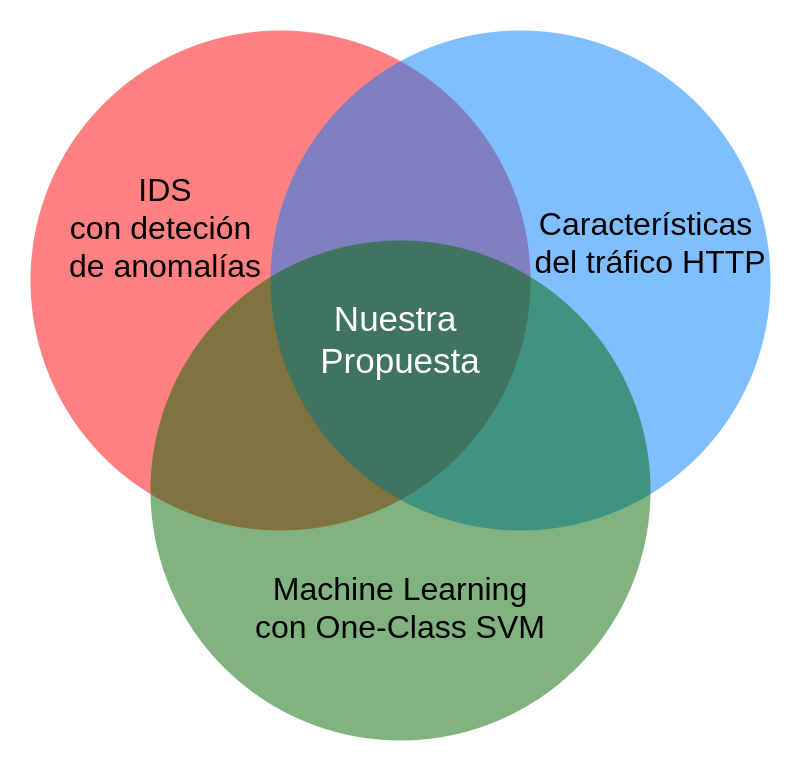
\includegraphics[width=0.5\linewidth]{images/venn-areas-de-estudio.png}

    \caption{Diagrama de las áreas de estudio de la investigación.}
    \label{fig:intro:areas_de_estudio}
\end{figure}

\begin{itemize}
    \item
    \gls{acr3:ids} con detección de anomalías:
    \gls{acr3:name} busca detectar posibles ataques al reconocerlos como
    mensajes anómalos. Utilizamos el método de detección de anomalías
    debido a sus ventajas que fueron mencionadas en la sección anterior.

    \item
    Características de los mensajes \gls{acr3:http}:
    \gls{acr3:name} utiliza conocimiento experto sobre la estructura de
    los mensajes \gls{acr3:http}, que puede ayudar para diferenciar los
    mensajes normales de las anomalías o ataques, como se puede observar
    en los trabajos  \citep{kruegel2003anomaly} y \citep{kruegel2005multi}.

    \item
    \gls{acr3:ml} con \gls{acr3:ocsvm}:
    la detección de mensajes anómalos se puede abordar como un problema
    de \gls{acr3:occ}, y para ese tipo de problemas el clasificador en
    cuestión ha sido empleado exitosamente por otros investigadores,
    obteniendo buenos resultados en la clasificación
    \citep{khan2014one}. % from section 4.3.2 - application domains
\end{itemize}

En los trabajos de Kruegel y Vigna se combina las dos primeras áreas
descritas anteriormente, \gls{acr3:ids} y características de los mensajes
\gls{acr3:http}. Sus aportes ya fueron utilizados y extendidos en varios
trabajos en años subsecuentes, pero nosotros no hemos encontrado una
investigación que combine dichos aportes con el ya mencionado clasificador
\gls{acr3:ocsvm}.

En nuestra opinión, un \gls{acr3:waf} que combina los aportes de Kruegel
y Vigna con este clasificador puede ser de gran utilidad para la detección
de posibles ataques y de esta forma brindar una herramienta para mayor
protección de las aplicaciones web.


\section{Objetivos}

\subsection{Objetivo general}

Detectar mensajes \gls{acr3:http} anómalos entre las aplicaciones web
y sus usuarios con el fin de mitigar los riesgos de ataques contra dichas
aplicaciones, utilizando un \gls{acr3:waf} basado en clasificadores
\gls{acr3:ocsvm}.


\subsection{Objetivos específicos}

\begin{enumerate}
    \item
    Diseñar procesos de extracción de características (\textit{features})
    específicamente para mensajes \gls{acr3:http}, basado en aportes de
    otros investigadores de la literatura.

    \item
    Implementar un \gls{acr3:waf} basado en anomalías, utilizando los
    procesos de extracción de \textit{features} diseñados junto con
    clasificadores \gls{acr3:ocsvm}.

    \item
    Evaluar la eficacia del \gls{acr3:waf} implementado en cuanto a la
    detección de mensajes \gls{acr3:http} anómalos.

    \item
    Analizar la viabilidad de utilizar el \gls{acr3:waf} implementado
    para detección de ataques en tiempo real.
\end{enumerate}


\section{Organización del trabajo}

Este trabajo está organizado de la siguiente manera:
en el \autoref{chap:p3_concepts_features} entramos en más detalles sobre
cómo utilizamos las características de los mensajes \gls{acr3:http} en
nuestros procesos de extracción de \textit{features}.
Luego, en el \autoref{chap:p3_concepts_ocsvm} describimos con más detalles
el clasificador \gls{acr3:ocsvm}, mostrando de qué manera lo empleamos
para la detección de mensajes anómalos.
El \autoref{chap:p3_new_waf} contiene la presentación del \gls{acr3:waf}
que construimos en el marco de este trabajo, describiendo varios detalles
de la implementación y mostrando de qué manera utilizamos los componentes
descritos en los capítulos \ref{chap:p3_concepts_features} y
\ref{chap:p3_concepts_ocsvm}.
Después de eso, en el \autoref{chap:p3_results}, describimos las pruebas
realizadas con nuestra implementación y exponemos los resultados que hemos
obtenido en cada una de ellas.
Finalizamos el presente trabajo con nuestras conclusiones en el
\autoref{chap:p3_conclusions}, agregando también algunas ideas que pueden
ser el punto de partida para trabajos futuros.

    \renewcommand{\newCommandChapterTitle}{Extracción de \textit{features} en el contexto HTTP}
\chapter{\newCommandChapterTitle}
\markright{\hfill \thechapter. \newCommandChapterTitle}
\label{chap:p3_concepts_features}


La extracción de \textit{features} consiste en obtener características
representativas de los datos originales
\citep{torranoGimenez2015study}. % from section 2.3.1 - feature extraction
En nuestro caso, las características de los mensajes \gls{acr3:http} deben
ser expresadas por medio de vectores numéricos para que los clasificadores
\gls{acr3:ocsvm} del \gls{acr3:name} puedan reconocer dichas características.
En \citep{rieck2009machine} % from section 2.2 - feature maps
se habla también de mapas de \textit{features} para referirse a esta
extracción de características; se presenta este proceso como funciones
que mapean el dominio de mensajes \gls{acr3:http} a un espacio vectorial
$\mathbb{R}^{n}$ de números reales, donde $1 \leq n \leq \infty$.

En este capítulo, en primer lugar damos algunas explicaciones sobre
la estructura de los mensajes \gls{acr3:http}, luego presentamos los
aportes de los trabajos de Kruegel y Vigna sobre las características
que utilizaron, y finalmente describimos los procesos de extracción de
\textit{features} que utiliza \gls{acr3:name} para realizar el mapeo de
mensajes a vectores numéricos.


\section{Estructura de mensajes HTTP}

El detector \gls{acr3:name} que presentamos en este trabajo analiza
mensajes \gls{acr3:http} y en esta sección introducimos los conceptos
necesarios sobre este protocolo de comunicación.
Nosotros solamente nos enfocamos en el protocolo \gls{acr3:http} en su
versión 1.1, en el cual los mensajes son enviados en formato de texto
\citep{fielding1999http}. % from the abstract

Además, \gls{acr3:name} analiza solamente los mensajes \gls{acr3:http}
que sean peticiones, ignorando los mensajes que sean respuestas. Debido
a que las peticiones son aquellos mensajes que llegan a las aplicaciones
web desde la Internet, estos pueden contener ataques; en cambio, los
mensajes de respuesta son generadas por las aplicaciones protegidas por
el \gls{acr3:waf} y por lo tanto hay menos riesgos de seguridad.
Obviando el análisis de las respuestas reducimos el procesamiento necesario
sin aumentar de forma significativa el riesgo de ataques.

Las peticiones \gls{acr3:http} pueden estar compuestas por seis partes:
un método \gls{acr3:http}, un identificador universal de recursos
(\gls{acr3:url} - \textit{Universal Resource Locator}), un \textit{query string},
la versión del protocolo, varias cabeceras y finalmente el cuerpo de la
petición \citep{fielding1999http}. % from section 5 - request
El método debe ser uno de los valores definidos para el protocolo; nuestro
\gls{acr3:waf} se enfoca solamente en peticiones con los métodos GET y POST,
ya que estos son los más utilizados.
La \gls{acr3:url} está compuesta por el indicador de protocolo, la dirección
del \textit{host}, el puerto y la ruta del recurso pedido (\textit{path}).
Las cabeceras son opcionales y permiten enviar información adicional sobre
la petición. Cada cabecera consiste en un nombre y su valor, separados por
el signo de dos puntos (:). Las cabeceras van delimitadas por los caracteres
de nueva linea (CRLF).

El \textit{query string}, que es opcional, va separado de la \gls{acr3:url}
mediante un signo de interrogación (?) y está compuesto por pares de
parámetros y valores. Estos parámetros están separados de sus valores
mediante el símbolo de igualdad (=), mientras que los pares se encuentran
delimitados por el símbolo \textit{ampersand} (\&). De esta forma, el
\textit{query string} de una petición puede ser representado como la lista
de pares ordenados
$\{ (p_{1}, v_{1}), (p_{2}, v_{2}), \dots , (p_{n}, v_{n}) \}$.
Estos parámetros son utilizados, por ejemplo, para pasar criterios de
filtrado y ordenación de datos a las aplicaciones.

Las peticiones del método GET no suelen llevar un cuerpo. Las peticiones
del método POST en algunos casos lo tienen, y en caso de contar con el
mismo, su contenido puede estar estructurado de varias formas posibles.
Para esta investigación consideramos únicamente los cuerpos de peticiones
POST que constan de pares de parámetros y valores estructurados de la
misma forma que el \textit{query string}. De esta manera, el cuerpo de
una petición puede ser expresado como la lista
$\{ (p_{1}, v_{1}), (p_{2}, v_{2}), \dots , (p_{n}, v_{n}) \}$.
En esta investigación, no analizamos cuerpos de peticiones con contenido
en otros formatos, por ejemplo aquellos que tengan datos binarios.
Los cuerpos de peticiones POST pueden ser utilizados, por ejemplo, para
enviar datos de formularios completados por usuarios a aplicaciones web.

\begin{figure}[htb]
    \centering
    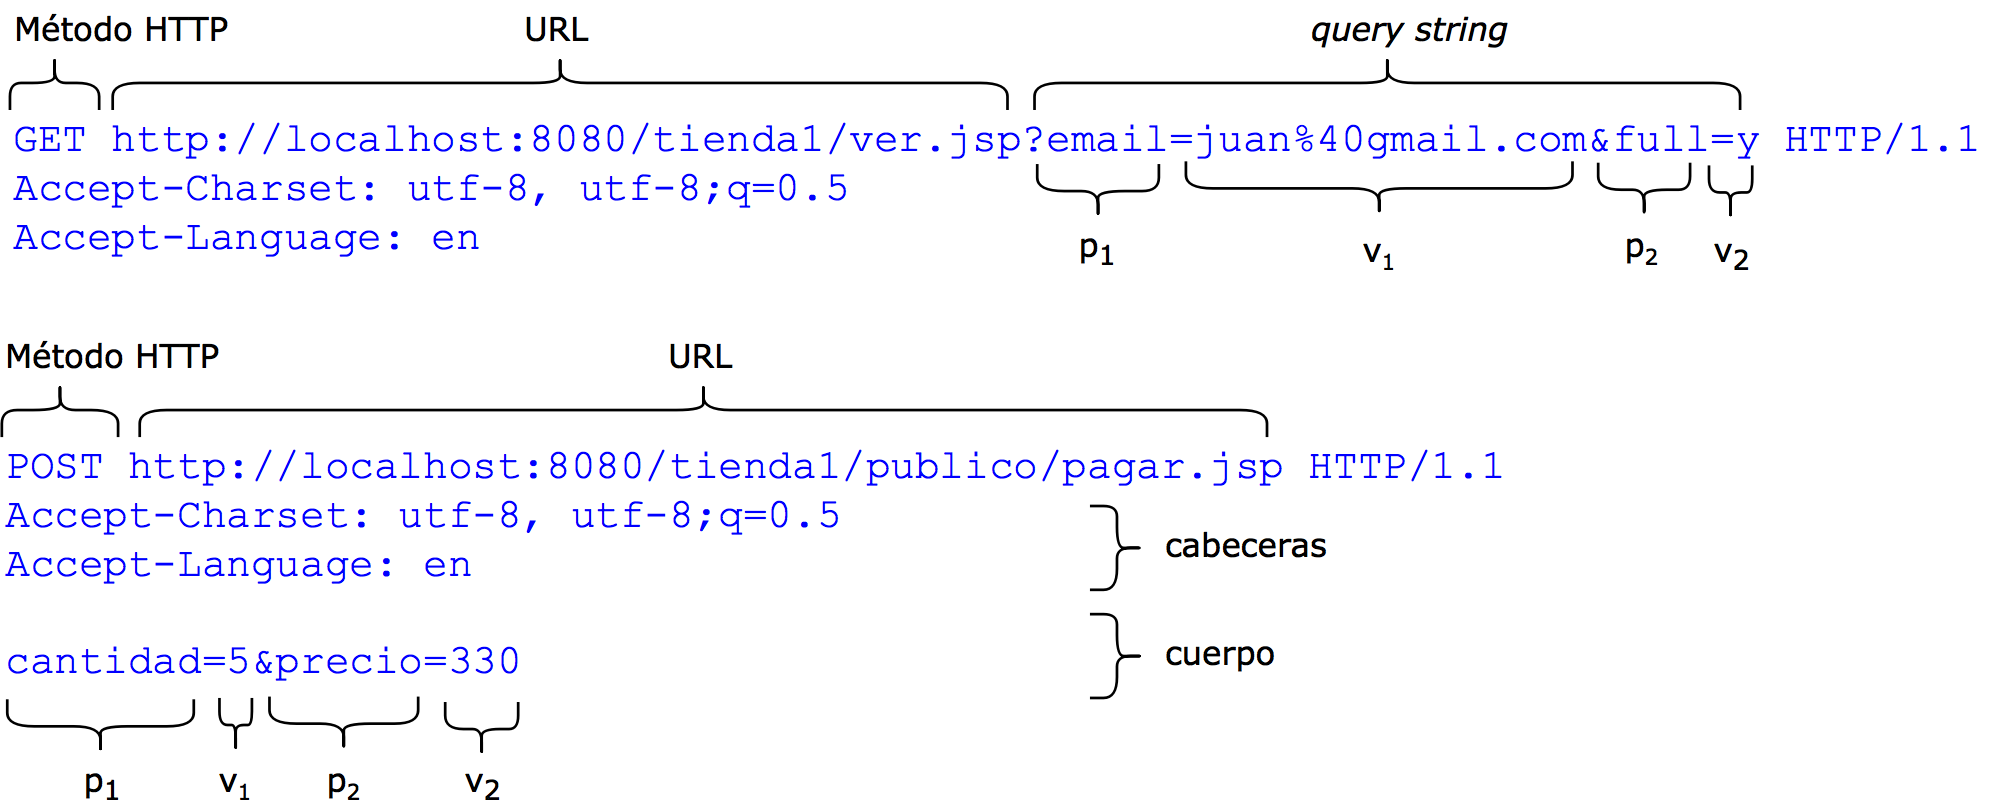
\includegraphics[width=\linewidth]{images/http-request-structure.png}

    \caption{Diagrama de estructura de dos peticiones \gls{acr3:http},
        una con método GET y otra con método POST.}
    \label{fig:fe:http_request_structure}
\end{figure}

En la \autoref{fig:fe:http_request_structure} se puede observar la estructura
de dos peticiones de ejemplo. La primera es una petición con el método GET.
La misma tiene un \textit{query string} con los dos parámetros \textit{email}
y \textit{full} con sus respectivos valores. Esta primera petición no
tiene cuerpo. La segunda petición tiene el método POST y no cuenta con un
\textit{query string}, pero en el cuerpo contiene los parámetros \textit{modo}
y \textit{precio} con sus valores. Ambas peticiones contienen dos cabeceras
que son \textit{Accept-Charset} y \textit{Accept-Language} con sus valores.
Cabe mencionar que los caracteres de la petición que tienen significado
especial en el contexto del mensaje deben ser reemplazados por un código
hexadecimal precedido por un símbolo de porcentaje (\%), un proceso conocido
como \textit{percent encoding}
\citep{bernerslee2005uri}. % from section 2.1 - percent encoding
Este reemplazo se puede observar en el valor del parámetro \textit{email}
de la primera petición de la figura mencionada, donde el símbolo @ queda
reemplazado por el código \%40.


\section{Características HTTP según Kruegel y Vigna}

Los autores Kruegel y Vigna presentaron varias ideas relacionadas a la
detección de anomalías en peticiones \gls{acr3:http}.
En los trabajos \citep{kruegel2003anomaly} y \citep{kruegel2005multi}
utilizan conocimiento experto sobre mensajes \gls{acr3:http},
específicamente sobre las peticiones, para construir modelos de anomalías
durante una fase de entrenamiento y luego, durante una fase de detección,
emplean esos modelos para obtener una detección eficaz.
Nosotros basamos nuestra propuesta en dos aspectos de sus aportes:
en primer lugar usamos el análisis de valores de parámetros del
\textit{query string} que ellos proponen y en segundo lugar empleamos
algunas de las características que ellos utilizan en sus modelos de
anomalías.

Cabe mencionar que Kruegel y Vigna utilizan métodos estadísticos para
la detección de anomalías y no herramientas de \gls{acr3:ml} como nosotros.
Debido a eso, ellos no utilizan vectores de \textit{features}.
Aun así, utilizamos los dos aspectos de sus aportes mencionados anteriormente
para mejorar nuestros procesos de extracción de \textit{features}, apuntando
a mejorar la detección de peticiones anómalas del \gls{acr3:name}.
Adicionalmente, Kruegel y Vigna realizan sus tareas de detección de
anomalías en base a archivos \textit{logs} de servidores \gls{acr3:http},
pero no trabajan sobre tráfico en tiempo real. Como en esos \textit{logs}
solamente había peticiones con el método GET, sus trabajos tratan únicamente
de ese tipo de peticiones.


\subsection{Análisis de valores de parámetros}

Los autores Kruegel y Vigna aplican sus modelos de anomalías sobre el
\textit{query string} de peticiones GET y además sobre los valores individuales
de los parámetros de la misma. En la fase de detección, sus modelos obtienen
una probabilidad de que el valor analizado pertenezca al conjuntos de valores
vistos durante el entrenamiento.

Durante la fase de entrenamiento, en primer lugar las peticiones
\gls{acr3:http} son agrupadas por método y \gls{acr3:url}; los autores
utilizaron solamente peticiones GET y así en la práctica su agrupación
fue por \gls{acr3:url} únicamente.
Esta agrupación se realiza ya que peticiones que van dirigidas a una misma
\gls{acr3:url} y con el mismo método \gls{acr3:http} presentan más
similitudes entre ellas que con peticiones que tienen otro método o
\gls{acr3:url}. De esta manera, se obtiene modelos de anomalías
independientes y más precisos dentro de cada grupo.
Después de agrupar, se realiza la extracción de los parámetros que aparecen
en el \textit{query string} de las peticiones dentro de cada grupo. Luego
se construye modelos de anomalías por cada uno de los parámetros extraídos,
utilizando los valores que dichos parámetros tienen en las peticiones del
conjunto de entrenamiento.
Por ejemplo, se analiza la longitud de todos los valores de un parámetro,
construyendo de esta forma un modelo de anomalía que utiliza promedio
y desviación estándar de las longitudes para definir a partir de qué
longitud un valor de ese parámetro específico será considerado anómalo.
Además, se tiene modelos aplicados al \textit{query string} completo,
como por ejemplo el análisis de presencia de parámetros.

Durante la fase de detección, el sistema propuesto por los autores
mencionados analiza las peticiones nuevas con los modelos construidos
previamente. Primeramente se busca el grupo al cual pertenece la petición,
luego se obtiene la lista de parámetros vistos durante el entrenamiento
para ese grupo y luego se extraen todos los valores que esos parámetros
tienen en la petición en cuestión. Después se aplican los modelos sobre
los valores, obteniendo resultados que indican la probabilidad de que
los nuevos valores sean normales.
Así, por cada parámetro de la petición se tendrá varios resultados calculados
por los distintos modelos, de los cuales se obtiene una probabilidad final
mediante una suma ponderada. Esta probabilidad final es comparada con un
umbral (\textit{threshold}) establecido previamente para decidir si la
petición analizada es normal o anómala.

En esta parte cabe resaltar que el análisis hecho por estos autores utiliza
una cantidad variable de modelos en cada grupo de peticiones, ya que cada
grupo puede tener una cantidad distinta de parámetros; esa cantidad de
parámetros observados durante el entrenamiento determina la cantidad de
modelos que se tendrá.
Este abordaje es diferente a otros trabajos relacionados al área de
\gls{acr3:ids} en donde se utiliza una cantidad fija de características
de los mensajes; podemos ver un ejemplo de esto en
\citep{nguyen2011application}, % from section 3 - experiments
donde se utiliza 30 \textit{features} de peticiones \gls{acr3:http}
para los distintos clasificadores empleados.


\subsection{Características analizadas de los mensajes}

Kruegel y Vigna analizan un total de nueve características distintas
en sus trabajos \citep{kruegel2003anomaly} y \citep{kruegel2005multi},
a partir de las cuales construyen sus modelos de anomalías; estas
características pueden ser observadas en la
\autoref{tbl:fe:kruegel_feature_list}.

Los autores detallan también los tipos de ataques que se busca detectar
con cada uno de sus modelos de anomalías. Entre los ataques detectados se
encuentran, por ejemplo, ataques de \textit{buffer overflow},
\textit{directory transversal}, \textit{cross-site scripting}
y también \textit{SQL injection}.

\begin{table}[ht]
    \centering
    \small
    \begin{tabularx}{\linewidth}{|X|c|}
        \hline
        \multicolumn{1}{|c|}{Características analizadas por Kruegel y Vigna}
        & Características utilizada en \gls{acr3:name} \\
        \specialrule{1.5pt}{0}{0}
        Longitud                            & Sí \\ \hline
        Distribución de caracteres          & Sí \\ \hline
        Inferencia de estructura            & -  \\ \hline
        Análisis de \textit{tokens}         & -  \\ \hline
        Presencia o ausencia de parámetros  & -  \\ \hline
        Orden de parámetros                 & -  \\ \hline
        Frecuencia de invocación            & -  \\ \hline
        Tiempo entre invocaciones           & -  \\ \hline
        Orden de invocación                 & -  \\ \hline
    \end{tabularx}

    \caption{Características de mensajes \gls{acr3:http} utilizadas por
        Kruegel y Vigna en sus modelos de anomalías, indicando también
        cuales de estas características son utilizadas en \gls{acr3:name}.}
    \label{tbl:fe:kruegel_feature_list}
\end{table}

En nuestra opinión, no todas las características presentadas son aplicables
a nuestro caso con herramientas de \gls{acr3:ml}. De esa forma, nosotros
empleamos solamente dos de las características de la tabla mencionada para
construir los procesos de extracción de \textit{features} del \gls{acr3:name};
estos procesos son presentados en la siguiente sección.


\section{Nuestros procesos de extracción de \textit{features}}

En esta sección presentamos los procesos que realizan la extracción de
\textit{features} en \gls{acr3:name}. Primeramente, describimos la agrupación
de peticiones que realizamos, luego explicamos el análisis de valores de
parámetros que hacemos y después detallamos los \textit{features} que
extraemos de cada uno de los valores.

A modo de ilustrar mejor los conceptos de esta sección, utilizamos un
conjunto de peticiones de ejemplo sobre el que aplicamos nuestros procesos
de extracción que presentamos a continuación. En la \autoref{tbl:fe:example_1}
se pueden observar dichas peticiones de ejemplo, que son 20 peticiones GET
que fueron hechas a una misma \gls{acr3:url}. De este conjunto, las primeras
15 peticiones son normales y las otras 5 contienen alguna anomalía o ataque.
Además, las primeras 10 peticiones normales serán utilizadas para la fase
de entrenamiento, mientras que las demás normales y las anomalías recién
serán utilizadas para la fase de detección.

\begin{table}[!th]
    \centering
    \fontsize{10}{12}\selectfont
    \begin{tabularx}{\linewidth}{|c|C|C|>{\ttfamily}l|}
        \hline
        ID & Clase    & Grupo         & \multicolumn{1}{c|}{Petición completa}                       \\
        \specialrule{1.5pt}{0}{0}
         1 & normal   & entrenamiento & GET http://localhost:8080/tienda1/miembros/ver.jsp?          \\
           &          &               & email=talmadge\%40movintel.uz HTTP/1.1                       \\ \hline
         2 & normal   & entrenamiento & GET http://localhost:8080/tienda1/miembros/ver.jsp?          \\
           &          &               & email=tarangelo\%40accesoabierto.st HTTP/1.1                 \\ \hline
         3 & normal   & entrenamiento & GET http://localhost:8080/tienda1/miembros/ver.jsp?          \\
           &          &               & email=tarasova\_dabo\%40comerciosdeaspe.ly HTTP/1.1          \\ \hline
         4 & normal   & entrenamiento & GET http://localhost:8080/tienda1/miembros/ver.jsp?          \\
           &          &               & email=tazaki\_waggenheim\%40telelujo.an HTTP/1.1             \\ \hline
         5 & normal   & entrenamiento & GET http://localhost:8080/tienda1/miembros/ver.jsp?          \\
           &          &               & email=tati\%40callalabocaatiaherminia.travel HTTP/1.1        \\ \hline
         6 & normal   & entrenamiento & GET http://localhost:8080/tienda1/miembros/ver.jsp?          \\
           &          &               & email=tauber5\%40lamolahotel.bb\&full=yes HTTP/1.1           \\ \hline
         7 & normal   & entrenamiento & GET http://localhost:8080/tienda1/miembros/ver.jsp?          \\
           &          &               & email=tayo\%4013horas.tn HTTP/1.1                            \\ \hline
         8 & normal   & entrenamiento & GET http://localhost:8080/tienda1/miembros/ver.jsp?          \\
           &          &               & email=tanimoto\_hassen\%40autobuses-hibridos.tw HTTP/1.1     \\ \hline
         9 & normal   & entrenamiento & GET http://localhost:8080/tienda1/miembros/ver.jsp?          \\
           &          &               & email=tarp\%40redstarz.asia\&full=yes HTTP/1.1               \\ \hline
        10 & normal   & entrenamiento & GET http://localhost:8080/tienda1/miembros/ver.jsp?          \\
           &          &               & email=teje-lipman\%40hojainformativas.sa HTTP/1.1            \\ \hline
        11 & normal   & detección     & GET http://localhost:8080/tienda1/miembros/ver.jsp?          \\
           &          &               & email=taneda\%40ajuntamentdebcn20.be HTTP/1.1                \\ \hline
        12 & normal   & detección     & GET http://localhost:8080/tienda1/miembros/ver.jsp?          \\
           &          &               & email=tannen\%40getgold.ua HTTP/1.1                          \\ \hline
        13 & normal   & detección     & GET http://localhost:8080/tienda1/miembros/ver.jsp?          \\
           &          &               & email=tchjan-lian.quadflieg\%40comerciosdeaspe.se HTTP/1.1   \\ \hline
        14 & normal   & detección     & GET http://localhost:8080/tienda1/miembros/ver.jsp?          \\
           &          &               & email=tarver\%40callofduty6.lb\&full=yes HTTP/1.1            \\ \hline
        15 & normal   & detección     & GET http://localhost:8080/tienda1/miembros/ver.jsp?          \\
           &          &               & email=tay\%40autobuses-hibridos.ps HTTP/1.1                  \\ \hline
        16 & anomalía & detección     & GET http://localhost:8080/tienda1/miembros/ver.jsp?          \\
           &          &               & email=\%27\%3B+DROP+TABLE+user\%3B+SELECT+*+FROM+p+WHERE+    \\
           &          &               & name+LIKE+\%27\%25 HTTP/1.1                                  \\ \hline
        17 & anomalía & detección     & GET http://localhost:8080/tienda1/miembros/ver.jsp?          \\
           &          &               & email=malformed1email2address3domain4 HTTP/1.1               \\ \hline
        18 & anomalía & detección     & GET http://localhost:8080/tienda1/miembros/ver.jsp?          \\
           &          &               & email=tayo\_1\%4013horas.tn\&full=12345\&show=no HTTP/1.1    \\ \hline
        19 & anomalía & detección     & GET http://localhost:8080/tienda1/miembros/ver.jsp?          \\
           &          &               & email=\%3C\%21--\%23exec+cmd\%3D\%22cat+\%2Fetc\%2Fpasswd+   \\
           &          &               & \%3E+somefile\%22+--\%3E HTTP/1.1                            \\ \hline
        20 & anomalía & detección     & GET http://localhost:8080/tienda1/miembros/ver.jsp?          \\
           &          &               & email=\%40cr\%40anh\%40am\%404horas.ki\&full=yes HTTP/1.1    \\ \hline
    \end{tabularx}

    \caption{Conjunto de 20 peticiones \gls{acr3:http} de ejemplo utilizadas
        para ilustrar el funcionamiento de \gls{acr3:name} en este trabajo.}
    \label{tbl:fe:example_1}
\end{table}


\subsection{Agrupación de peticiones}

Basado en los trabajos de Kruegel y Vigna mencionados en la sección
anterior, \gls{acr3:name} también realiza la agrupación de las peticiones
\gls{acr3:http} por método y \gls{acr3:url}. De esta forma, a partir de
las peticiones utilizadas para el entrenamiento, \gls{acr3:name} crea
un conjunto \gls{sim3:g} de grupos de peticiones, que contiene todos
los grupos de peticiones obtenidos mediante la agrupación de los datos
de entrenamiento.

Con esta agrupación podemos lograr una descripción más precisa de las
peticiones normales dentro de cada grupo \gls{sim3:gi}. Esto posibilita
inclusive la identificación de aquellas peticiones que, por ejemplo, son
anómalas dentro de su grupo correspondiente $G_{1}$, pero que podrían ser
consideradas normales en el contexto de otro grupo $G_{2}$.

En el caso de nuestras 20 peticiones de ejemplo, todas ellas fueron hechas
con el método GET a una sola \gls{acr3:url}. Por lo tanto, dichas peticiones
pertenecen al mismo grupo. Cabe volver a mencionar que para el entrenamiento
utilizamos las 10 primeras peticiones normales.


\subsection{Extracción de valores de los parámetros del \textit{query string}
    y cuerpo de las peticiones}

Con la agrupación realizada, partimos de la base de que las peticiones
dentro de un grupo \gls{sim3:gi} presentan gran similitud entre ellas.
Específicamente, se espera que esas peticiones tengan los mismos parámetros
en \textit{query string} y cuerpo, o que por lo menos no haya mucha
variación. Por ejemplo, en una \gls{acr3:url} para inicio de sesión,
todas las peticiones con el método POST deberían contener los parámetros
\textit{username} y \textit{password} en su cuerpo.

Como ya se mencionó en la sección anterior, Kruegel y Vigna utilizan
solamente peticiones GET en sus trabajos. \gls{acr3:name} incluye el
análisis de parámetros del cuerpo de las peticiones POST.
Cabe mencionar que estamos conscientes del riesgo de seguridad que puede
presentar el hecho de que se analice el cuerpo de peticiones POST, ya
que los mismos pueden contener información confidencial, como por ejemplo
contraseñas de acceso de usuarios. Para ajustarse a las necesidades de
las distintas situaciones, \gls{acr3:name} puede ser configurado para
excluir ciertos métodos \gls{acr3:http} o ciertas \gls{acr3:url}s del
análisis que realiza. Estas configuraciones quedan a cargo de los
administradores del \gls{acr3:name}.

De esta forma, en la fase de entrenamiento se construyen listas de todos
los parámetros que aparecen en las peticiones \gls{acr3:http} dentro
de cada grupo. La lista \gls{sim3:qi} contiene de forma ordenada todos
los parámetros que aparecen en el \textit{query string} de alguna
petición dentro del grupo \gls{sim3:gi}, excluyendo las duplicaciones.
De forma análoga, la lista \gls{sim3:bi} contiene los parámetros que
aparecen en el cuerpo de alguna petición del grupo.
Es posible que estas listas queden vacías para un grupo, lo que sucede
cuando ninguna petición contiene parámetros. En nuestras 10 peticiones
de ejemplo para el entrenamiento, \gls{sim3:qi} contiene los dos parámetros
\textit{email} y \textit{full}, pero \gls{sim3:bi} queda vacío porque las
peticiones no tienen cuerpo con parámetros.
Como ya mencionamos, se espera que los mismos parámetros se repitan en la
mayoría de las peticiones, de manera que estas listas de parámetros de un
grupo no sean mucho más extensas que la cantidad de parámetros de una sola
petición de dicho grupo.

Después de construir estas listas, se procesan las peticiones de cada
grupo \gls{sim3:gi} para construir los conjuntos de vectores \gls{sim3:fi},
en donde cada petición está representada por un vector de \textit{features}
\gls{sim3:fij}.
Por cada petición en \gls{sim3:gi}, se extraen los valores cuyos parámetros
aparezcan en las listas \gls{sim3:qi} y \gls{sim3:bi}. Luego se extraen
\gls{sim3:m} \textit{features} de cada uno de esos valores, añadiéndolos
de forma ordenada para formar el vector \gls{sim3:fij}. Esos \gls{sim3:m}
\textit{features} que utilizamos serán explicados en detalle en la
siguiente sección.

Con este análisis de los valores individuales de los parámetros se puede
detectar una gran cantidad de ataques que podrían estar presentes en el
\textit{query string} o en el cuerpo de las peticiones. Sin embargo, este
abordaje no cubre los casos de parámetros que no fueron observados durante
la fase entrenamiento, o aquellos ataques ocultos en otras partes de la
petición, por ejemplo en las cabeceras de mensajes.
Con el fin de mitigar esos riesgos, se extrae también los \gls{sim3:m}
\textit{features} de la petición \gls{acr3:http} completa, incluyendo
cada una de las seis partes que puede tener dicha petición.

De esta forma, cada petición de \gls{sim3:gi} queda representada por un
vector \gls{sim3:fij}, que se encuentra en el espacio $\mathbb{R}^{n}$.
La dimensión $n$ del espacio para cada uno de los grupo de peticiones,
representada por \gls{sim3:ni}, indica la cantidad de componentes de cada
\gls{sim3:fij} $\in$ \gls{sim3:fi} y esta dimensión está dada por la
expresión de la
\autoref{eq:fe:number_of_features}.

\begin{equation}
    \label{eq:fe:number_of_features}
    n_{i}
    =
    m
    \times
    \left(
        1 + \lvert Q_{i} \rvert + \lvert B_{i} \rvert
    \right)
\end{equation}

En esta ecuación, \gls{sim3:m} es la cantidad de \textit{features}
extraídos de cada valor que analizamos; el número 1 representa la petición
completa; $\lvert Q_{i} \rvert$ y $\lvert B_{i} \rvert$ son las cantidades
de parámetros en \gls{sim3:qi} y \gls{sim3:bi} respectivamente. Esta
cantidad de componentes \gls{sim3:ni} puede ser distinta en cada grupo
\gls{sim3:gi}, ya que depende de la cantidad de parámetros que se
encuentran en las peticiones de esos grupos.
Para nuestras peticiones de ejemplo, $\lvert Q_{i} \rvert = 2$ y
$\lvert B_{i} \rvert = 0$, de manera que $n_{i} = m \times 3$. Así,
cada petición será representada por vectores de $m \times 3$ componentes.
Recalcamos que los \gls{sim3:m} \textit{features} serán presentados más
adelante en esta sección.

En la fase de detección, para cada petición a analizar se construye un
vector de \textit{features} que las represente. Se respeta el orden
de los parámetros en \gls{sim3:qi} y \gls{sim3:bi} según el grupo
\gls{sim3:gi} al que pertenecen las peticiones. Si una petición tiene
un parámetro que no se vio en entrenamiento, el valor de este parámetro
no es analizado por separado, sino que su contenido solamente se considera
dentro del análisis de la petición completa. Este es el caso de nuestra
petición de ejemplo número 18, que tiene el parámetro \textit{show} que
no aparece en el entrenamiento.
En cambio, si un parámetro visto durante la fase de entrenamiento no
aparece en nuevas peticiones, los vectores de \textit{features} llevarán
0 en todos los componentes que correspondan a ese parámetro. En nuestros
ejemplos, el parámetro \textit{full} solamente aparece en algunas de
las peticiones y sus componentes correspondientes llevarán un 0 cuando
no está presente.
De esta forma, los vectores de \textit{features} siempre tendrán la
dimensión \gls{sim3:ni} que corresponde a su grupo.


\subsection{\textit{Features} extraídos de cada valor}

La petición \gls{acr3:http} completa y también cada uno de los valores de
los parámetros del \textit{query string} y del cuerpo son analizados y
mapeados a distintos componentes de los vectores \gls{sim3:fij}. Como
ya fue mencionado, de cada uno de estos valores se extraen \gls{sim3:m}
\textit{features}.
Dentro de nuestros procesos de extracción de \textit{features} utilizamos
10 números para representar cada valor, resultando en $m = 10$. En la
\autoref{tbl:fe:feature_list} se detallan estos 10 \textit{features}
que utilizamos, los cuales serán explicados más adelante en este capítulo.

Para la extracción de esos 10 \textit{features} de cada valor, utilizamos
tres funciones que retornan uno o más números cada una; específicamente
se tiene la primera función que analiza la distribución de caracteres,
la segunda función que calcula la entropía del valor y por último la
tercera función que analiza la cantidad de caracteres. Estas funciones
son presentadas en detalle a continuación.
Cabe mencionar que los valores son analizados después revertir el
\textit{percent encoding}, es decir, después de sustituir los códigos
hexadecimales precedidos por porcentaje con sus símbolos correspondientes.

\begin{table}[htb]
    \centering
    \small
    \begin{tabularx}{\linewidth}{|X|c|c|}
        \hline
        \multicolumn{1}{|c|}{\textit{Features}}     & Tipo de dato obtenido & Rango de valores \\ \specialrule{1.5pt}{0}{0}
        Distribución de caracteres - intervalo 0    & números reales        & $[0, 1]$         \\ \hline
        Distribución de caracteres - intervalo 1    & números reales        & $[0, 1]$         \\ \hline
        Distribución de caracteres - intervalo 2    & números reales        & $[0, 1]$         \\ \hline
        Distribución de caracteres - intervalo 3    & números reales        & $[0, 1]$         \\ \hline
        Distribución de caracteres - intervalo 4    & números reales        & $[0, 1]$         \\ \hline
        Entropía                                    & números reales        & $[0, \infty)$    \\ \hline
        Longitud o cantidad total de caracteres     & números enteros       & $[0, \infty)$    \\ \hline
        Cantidad de dígitos presentes               & números enteros       & $[0, \infty)$    \\ \hline
        Cantidad de letras presentes                & números enteros       & $[0, \infty)$    \\ \hline
        Cantidad de otros caracteres presentes      & números enteros       & $[0, \infty)$    \\ \hline
    \end{tabularx}

    \caption{Lista de 10 \textit{features} extraídos por nuestros procesos
        de extracción de \textit{features} de cada valor analizado.}
    \label{tbl:fe:feature_list}
\end{table}


\subsubsection{Distribución de caracteres}

La distribución de las frecuencias relativas de caracteres puede ser un
indicador acerca de la regularidad de la estructura del valor analizado.
No se analiza la frecuencia de aparición de los valores individuales, sino
que se toma en cuenta la relación entre las frecuencias de los caracteres
\citep{kruegel2003anomaly}. % from section 4.2

Para este fin, primeramente se obtiene las frecuencias relativas de cada
carácter distinto que aparece en el valor a analizar, es decir, para cada
carácter se cuenta sus apariciones dentro del valor en cuestión y se
divide esas cantidades por la longitud del valor, de modo que la suma
de todas las frecuencias equivale a 1. Luego, esta lista de frecuencias
es ordenada en forma descendente.

Se puede esperar que esta distribución de caracteres obtenida tenga una
disminución gradual para valores normales. Si un ataque de \textit{buffer overflow}
introduciría muchas repeticiones del mismo carácter, la distribución de ese
valor tendría una caída pronunciada después de la primera frecuencia en la
lista. De forma contraria, si el ataque introduciría un valor largo generado
de forma aleatoria, su distribución sería anómala por poseer casi ninguna
variación entre las frecuencias.

En la \autoref{tbl:fe:char_dis_example_1} se puede ver la distribución de
caracteres de un valor de ejemplo, \textit{empleado@empresa.com}. Este
valor tiene una longitud de 20 caracteres, con 12 caracteres diferentes.
Cada carácter diferente tiene su propia columna, junto con la frecuencia
relativa correspondiente. Las posiciones en la lista de frecuencias
inician en 0.

\begin{table}[ht]
    \centering
    \small
    \begin{tabularx}{\linewidth}{C|c|c|c|c|c|c|c|c|c|c|c|c}
        Posición   & 0         & 1          & 2         & 3         & 4         & 5          & 6          & 7          & 8          & 9          & 10         & 11 \\ \hline
        Carácter   & e         & m          & a         & o         & p         & c          & d          & l          & r          & s          & .          & @  \\ \hline
        Frecuencia & \num{0.2} & \num{0.15} & \num{0.1} & \num{0.1} & \num{0.1} & \num{0.05} & \num{0.05} & \num{0.05} & \num{0.05} & \num{0.05} & \num{0.05} & \num{0.05}
    \end{tabularx}

    \caption{Distribución de caracteres del valor \textit{empleado@empresa.com}.}
    \label{tbl:fe:char_dis_example_1}
\end{table}

En este punto, los autores Kruegel y Vigna proponen agrupar las frecuencias
relativas en intervalos o \textit{bins} de distintos tamaños.
Nosotros utilizamos cinco intervalos para esta agrupación de frecuencias.
La \autoref{tbl:fe:char_dis_example_2} se puede observar los intervalos,
las posiciones de la distribución que son sumadas en cada intervalo y
también muestra las sumas obtenidas con el valor de ejemplo que se mencionó.

\begin{table}[ht]
    \centering
    \small
    \begin{tabularx}{\linewidth}{C|c|c|c|c|c}
                             & Intervalo 0 & Intervalo 1 & Intervalo 2 & Intervalo 3 & Intervalo 4 \\ \hline
        Posiciones agrupadas & 0           & 1 y 2       & 3, 4 y 5    & 6, 7, 8 y 9 & 10 al último \\ \hline
        Suma de frecuencias  & \num{0.2}   & \num{0.25}  & \num{0.25}  & \num{0.2}   & \num{0.1}
    \end{tabularx}

    \caption{Agrupación de la distribución de caracteres para el valor
        de ejemplo \textit{empleado@empresa.com}.}
    \label{tbl:fe:char_dis_example_2}
\end{table}

Por otro lado, en la \autoref{tbl:fe:char_dis_example_3} podemos ver los
intervalos de un valor que contiene un ataque de \textit{buffer overflow}
que consta de muchas repeticiones de un solo carácter. Se puede observar
que el ataque contiene un número \num{1.0} en el intervalo 0, que es
mucho más elevado que los números en los demás intervalos, que todos
contienen \num{0.0}. Esta caída abrupta no se observa con el valor de
ejemplo normal, y de esta forma se puede detectar la anomalía.

\begin{table}[ht]
    \centering
    \small
    \begin{tabularx}{\linewidth}{C|c|c|c|c|c}
                             & Intervalo 0 & Intervalo 1 & Intervalo 2 & Intervalo 3 & Intervalo 4 \\ \hline
        Posiciones agrupadas & 0           & 1 y 2       & 3, 4 y 5    & 6, 7, 8 y 9 & 10 al último \\ \hline
        Suma de frecuencias  & \num{1.0}   & \num{0.0}   & \num{0.0}   & \num{0.0}   & \num{0.0}
    \end{tabularx}

    \caption{Agrupación de la distribución de caracteres de un valor de
        ejemplo que contiene un ataque de \textit{buffer overflow}.}
    \label{tbl:fe:char_dis_example_3}
\end{table}

A partir de este punto los autores mencionados obtienen una distribución
promedio en la fase de entrenamiento y aplican el método estadístico
$\chi^{2}$ de Pearson \citep{encyMathChi2} para comparar ese promedio
con las distribuciones obtenidas de los valores en la fase de detección.
En cambio, nuestra función que analiza la distribución de caracteres
retorna directamente las cinco sumas obtenidas en los cinco intervalos
para cada valor. Esos números son cinco componentes del vector \gls{sim3:fij}
que representa una petición; posteriormente, el vector será utilizado
por el clasificador \gls{acr3:ocsvm} para analizar si es una petición
normal o anómala.

En la \autoref{tbl:fe:example_char_dis} se puede observar los \textit{features}
de distribución de caracteres extraídos de nuestras peticiones de ejemplo.
Las primeras 10 peticiones fueron utilizadas para el entrenamiento,
mientras que las demás peticiones fueron analizadas con los parámetros
encontrados en entrenamiento.
Cada fila de la tabla representa 15 componentes del vector de \textit{features}
de la petición correspondiente. Mostramos los números redondeados a dos
dígitos de precisión, a pesar de que nuestra implementación utiliza todos
los decimales disponibles.

En esta parte queda también ilustrado el comportamiento de nuestros
procesos de extracción de \textit{features} frente a la aparición de
parámetros en la fase de detección que no se observaron durante la fase
de entrenamiento. Se puede notar que la petición de ejemplo número 18
de la \autoref{tbl:fe:example_1} tiene el parámetro \textit{show}, pero
como este parámetro no aparece entre la peticiones de entrenamiento, el
mismo no tiene sus propios componentes en el vector de \textit{features}
(y tampoco sus propias columnas en la \autoref{tbl:fe:example_char_dis}
en cuestión).

\begin{table}[ht]
    \centering
    \small
    \begin{tabularx}{\linewidth}{|C|r|r|r|}
        \hline
        ID & \multicolumn{1}{c|}{Petición completa}                                             & \multicolumn{1}{c|}{Parámetro \textit{email}}                                      & \multicolumn{1}{c|}{Parámetro \textit{full}} \\ \specialrule{1.5pt}{0}{0}
         1 & \num{0.07} \space \num{0.14} \space \num{0.17} \space \num{0.16} \space \num{0.47} & \num{0.10} \space \num{0.20} \space \num{0.25} \space \num{0.20} \space \num{0.25} & \num{0.00} \space \num{0.00} \space \num{0.00} \space \num{0.00} \space \num{0.00} \\ \hline
         2 & \num{0.07} \space \num{0.15} \space \num{0.18} \space \num{0.16} \space \num{0.44} & \num{0.15} \space \num{0.23} \space \num{0.27} \space \num{0.19} \space \num{0.15} & \num{0.00} \space \num{0.00} \space \num{0.00} \space \num{0.00} \space \num{0.00} \\ \hline
         3 & \num{0.08} \space \num{0.14} \space \num{0.17} \space \num{0.16} \space \num{0.45} & \num{0.16} \space \num{0.22} \space \num{0.22} \space \num{0.16} \space \num{0.25} & \num{0.00} \space \num{0.00} \space \num{0.00} \space \num{0.00} \space \num{0.00} \\ \hline
         4 & \num{0.08} \space \num{0.13} \space \num{0.16} \space \num{0.14} \space \num{0.47} & \num{0.14} \space \num{0.21} \space \num{0.21} \space \num{0.17} \space \num{0.28} & \num{0.00} \space \num{0.00} \space \num{0.00} \space \num{0.00} \space \num{0.00} \\ \hline
         5 & \num{0.12} \space \num{0.15} \space \num{0.18} \space \num{0.15} \space \num{0.41} & \num{0.26} \space \num{0.23} \space \num{0.23} \space \num{0.14} \space \num{0.14} & \num{0.00} \space \num{0.00} \space \num{0.00} \space \num{0.00} \space \num{0.00} \\ \hline
         6 & \num{0.08} \space \num{0.13} \space \num{0.17} \space \num{0.15} \space \num{0.46} & \num{0.14} \space \num{0.27} \space \num{0.27} \space \num{0.18} \space \num{0.14} & \num{0.33} \space \num{0.67} \space \num{0.00} \space \num{0.00} \space \num{0.00} \\ \hline
         7 & \num{0.07} \space \num{0.13} \space \num{0.16} \space \num{0.16} \space \num{0.48} & \num{0.13} \space \num{0.27} \space \num{0.20} \space \num{0.27} \space \num{0.13} & \num{0.00} \space \num{0.00} \space \num{0.00} \space \num{0.00} \space \num{0.00} \\ \hline
         8 & \num{0.08} \space \num{0.14} \space \num{0.17} \space \num{0.16} \space \num{0.45} & \num{0.14} \space \num{0.22} \space \num{0.22} \space \num{0.22} \space \num{0.22} & \num{0.00} \space \num{0.00} \space \num{0.00} \space \num{0.00} \space \num{0.00} \\ \hline
         9 & \num{0.07} \space \num{0.13} \space \num{0.18} \space \num{0.16} \space \num{0.46} & \num{0.22} \space \num{0.28} \space \num{0.22} \space \num{0.22} \space \num{0.06} & \num{0.33} \space \num{0.67} \space \num{0.00} \space \num{0.00} \space \num{0.00} \\ \hline
        10 & \num{0.08} \space \num{0.12} \space \num{0.17} \space \num{0.17} \space \num{0.45} & \num{0.16} \space \num{0.16} \space \num{0.19} \space \num{0.23} \space \num{0.26} & \num{0.00} \space \num{0.00} \space \num{0.00} \space \num{0.00} \space \num{0.00} \\ \hline
        11 & \num{0.08} \space \num{0.15} \space \num{0.16} \space \num{0.14} \space \num{0.47} & \num{0.15} \space \num{0.30} \space \num{0.26} \space \num{0.15} \space \num{0.15} & \num{0.00} \space \num{0.00} \space \num{0.00} \space \num{0.00} \space \num{0.00} \\ \hline
        12 & \num{0.07} \space \num{0.14} \space \num{0.15} \space \num{0.15} \space \num{0.48} & \num{0.18} \space \num{0.24} \space \num{0.29} \space \num{0.24} \space \num{0.06} & \num{0.00} \space \num{0.00} \space \num{0.00} \space \num{0.00} \space \num{0.00} \\ \hline
        13 & \num{0.08} \space \num{0.12} \space \num{0.16} \space \num{0.17} \space \num{0.47} & \num{0.12} \space \num{0.17} \space \num{0.20} \space \num{0.20} \space \num{0.30} & \num{0.00} \space \num{0.00} \space \num{0.00} \space \num{0.00} \space \num{0.00} \\ \hline
        14 & \num{0.08} \space \num{0.12} \space \num{0.15} \space \num{0.14} \space \num{0.50} & \num{0.14} \space \num{0.19} \space \num{0.19} \space \num{0.19} \space \num{0.29} & \num{0.33} \space \num{0.67} \space \num{0.00} \space \num{0.00} \space \num{0.00} \\ \hline
        15 & \num{0.08} \space \num{0.13} \space \num{0.16} \space \num{0.15} \space \num{0.48} & \num{0.16} \space \num{0.16} \space \num{0.24} \space \num{0.20} \space \num{0.24} & \num{0.00} \space \num{0.00} \space \num{0.00} \space \num{0.00} \space \num{0.00} \\ \hline
        16 & \num{0.08} \space \num{0.10} \space \num{0.12} \space \num{0.12} \space \num{0.57} & \num{0.20} \space \num{0.17} \space \num{0.13} \space \num{0.13} \space \num{0.37} & \num{0.00} \space \num{0.00} \space \num{0.00} \space \num{0.00} \space \num{0.00} \\ \hline
        17 & \num{0.07} \space \num{0.14} \space \num{0.16} \space \num{0.20} \space \num{0.42} & \num{0.13} \space \num{0.26} \space \num{0.23} \space \num{0.23} \space \num{0.16} & \num{0.00} \space \num{0.00} \space \num{0.00} \space \num{0.00} \space \num{0.00} \\ \hline
        18 & \num{0.07} \space \num{0.12} \space \num{0.15} \space \num{0.15} \space \num{0.51} & \num{0.12} \space \num{0.24} \space \num{0.24} \space \num{0.24} \space \num{0.18} & \num{0.20} \space \num{0.40} \space \num{0.40} \space \num{0.00} \space \num{0.00} \\ \hline
        19 & \num{0.08} \space \num{0.13} \space \num{0.14} \space \num{0.15} \space \num{0.51} & \num{0.11} \space \num{0.20} \space \num{0.20} \space \num{0.17} \space \num{0.33} & \num{0.00} \space \num{0.00} \space \num{0.00} \space \num{0.00} \space \num{0.00} \\ \hline
        20 & \num{0.06} \space \num{0.12} \space \num{0.15} \space \num{0.17} \space \num{0.51} & \num{0.20} \space \num{0.25} \space \num{0.20} \space \num{0.20} \space \num{0.15} & \num{0.33} \space \num{0.67} \space \num{0.00} \space \num{0.00} \space \num{0.00} \\ \hline
    \end{tabularx}

    \caption{Distribución de caracteres de nuestras 20 peticiones de ejemplo.}
    \label{tbl:fe:example_char_dis}
\end{table}


\subsubsection{Entropía}

La entropía de un valor, en el contexto de la teoría de la información,
nos indica la cantidad de información que puede contener dicho valor,
relacionando la longitud del valor con la cantidad de símbolos o caracteres
distintos presentes en el mismo.
La \autoref{eq:fe:entropy} muestra la fórmula utilizada para calcular
la entropía, propuesta por Claude Shannon hace varias décadas
\citep{encyMathEntropy}.

\begin{equation}
    \label{eq:fe:entropy}
    H(x) =
    - \sum_{i=1}^{n}
    \left(
        \frac{c_{i}}{n} \times \log_{2} \frac{c_{i}}{n}
    \right)
\end{equation}

En la ecuación mencionada, el símbolo $x$ representa el valor del cual
se calcula la entropía (que en nuestro caso son cadenas de caracteres),
el símbolo $n$ es la cantidad de caracteres distintos que se puede encontrar
en el valor $x$, mientras que $c_{i}$ indica la cantidad de ocurrencias
o apariciones de un mismo carácter $i$ dentro del valor $x$.

La entropía toma valores positivos, donde números cercanos a 0 indican
que hay muchas repeticiones de algunos pocos caracteres, mientras que
números mayores de entropía resultan de una mayor diversidad de caracteres
dentro del valor analizado.

Podemos observar las entropías de algunos valores de ejemplo en la
\autoref{tbl:fe:entropy_example_1}. Por ejemplo, comparando los valores
\textit{emp} y \textit{empempempempempempem} notamos que tienen la misma
cantidad de caracteres distintos y la misma entropía, a pesar de que el
segundo tiene mayor longitud.

Eso nos muestra que una mayor longitud del valor no es suficiente para
obtener mayores números para la entropía, sino que se necesita también
una mayor variación en su contenido. Cabe resaltar que, como se puede
observar en los primeros tres valores de la tabla, la presencia de un
único carácter resulta en una entropía igual a 0.

\begin{table}[ht]
    \centering
    \small
    \begin{tabular}{c|c|c|c}
        Valor                   & Longitud & Caracteres distintos & Entropía   \\
        \specialrule{1.5pt}{0}{0}
        e                       & \num{1}  & \num{1}              & \num{0.00} \\ \hline
        ee                      & \num{2}  & \num{1}              & \num{0.00} \\ \hline
        eeeeeeeeeeeeeeeeeeee    & \num{20} & \num{1}              & \num{0.00} \\ \hline
        empleado                & \num{8}  & \num{7}              & \num{2.75} \\ \hline
        empleadooooooooooooo    & \num{20} & \num{7}              & \num{1.82} \\ \hline
        emp                     & \num{3}  & \num{3}              & \num{1.58} \\ \hline
        empempempempempempem    & \num{20} & \num{3}              & \num{1.58} \\ \hline
        empleado@empresa.com    & \num{20} & \num{12}             & \num{3.38} \\ \hline
        abcdefghijklmnopqrst    & \num{20} & \num{20}             & \num{4.32}
    \end{tabular}

    \caption{Entropías de valores de ejemplo.}
    \label{tbl:fe:entropy_example_1}
\end{table}

En el trabajo \citep{nguyen2011application} % from section 3 - experiments
se utiliza la entropía como una de las varias métricas empleadas en su
sistema de detección de anomalías.
Esta medida puede ayudar a detectar, por ejemplo, un valor que contiene
un ataque de \textit{buffer overflow} que consta de muchas repeticiones
de un solo carácter. Para estos casos la entropía del valor será más baja
que en los valores normales observados durante el entrenamiento.

Nuestros procesos de extracción de \textit{features} calculan la entropía
y retorna ese número para cada valor analizado.
En la \autoref{tbl:fe:example_entropy} se puede observar los \textit{features}
de entropía extraídos de nuestras peticiones de ejemplo. De vuelta,
utilizamos las primeras 10 peticiones para el entrenamiento, mientras
que las demás fueron analizadas con los parámetros encontrados en
entrenamiento. Cada fila contiene tres componentes del vector \gls{sim3:fij}
de la petición correspondiente.
Mostramos los números redondeados a dos dígitos de precisión, a pesar de que
nuestra implementación utiliza todos los decimales disponibles.

\begin{table}[ht]
    \centering
    \small
    \begin{tabularx}{\linewidth}{|C|c|c|c|}
        \hline
        ID de la petición & Petición completa & Parámetro \textit{email} & Parámetro \textit{full} \\ \specialrule{1.5pt}{0}{0}
         1                & \num{4.88}        & \num{3.82}               & \num{0.00}              \\ \hline
         2                & \num{4.77}        & \num{3.61}               & \num{0.00}              \\ \hline
         3                & \num{4.81}        & \num{3.90}               & \num{0.00}              \\ \hline
         4                & \num{4.94}        & \num{3.96}               & \num{0.00}              \\ \hline
         5                & \num{4.66}        & \num{3.46}               & \num{0.00}              \\ \hline
         6                & \num{4.90}        & \num{3.54}               & \num{1.58}              \\ \hline
         7                & \num{4.85}        & \num{3.51}               & \num{0.00}              \\ \hline
         8                & \num{4.85}        & \num{3.94}               & \num{0.00}              \\ \hline
         9                & \num{4.90}        & \num{3.24}               & \num{1.58}              \\ \hline
        10                & \num{4.81}        & \num{3.97}               & \num{0.00}              \\ \hline
        11                & \num{4.83}        & \num{3.54}               & \num{0.00}              \\ \hline
        12                & \num{4.86}        & \num{3.34}               & \num{0.00}              \\ \hline
        13                & \num{4.91}        & \num{4.23}               & \num{0.00}              \\ \hline
        14                & \num{4.98}        & \num{3.88}               & \num{1.58}              \\ \hline
        15                & \num{4.88}        & \num{3.84}               & \num{0.00}              \\ \hline
        16                & \num{5.36}        & \num{4.40}               & \num{0.00}              \\ \hline
        17                & \num{4.77}        & \num{3.70}               & \num{0.00}              \\ \hline
        18                & \num{5.07}        & \num{3.62}               & \num{2.32}              \\ \hline
        19                & \num{5.03}        & \num{4.26}               & \num{0.00}              \\ \hline
        20                & \num{4.97}        & \num{3.48}               & \num{1.58}              \\ \hline
    \end{tabularx}

    \caption{Entropía de nuestras 20 peticiones de ejemplo.}
    \label{tbl:fe:example_entropy}
\end{table}


\subsubsection{Cantidad de caracteres}

En \citep{kruegel2003anomaly} % from section 4.1
se utiliza la longitud de valores como un indicador de anomalías. La
longitud puede ser entendida también como la cantidad total de caracteres
del valor. En \citep{nguyen2011application} % from section 3 - experiments
se extraen algunas características de las peticiones \gls{acr3:http} que
cuentan un subconjunto de caracteres, por ejemplo, uno de los \textit{features}
que utilizan es la cantidad de dígitos presentes en el \textit{path}
de la petición, mientras que otro \textit{feature} indica la cantidad
total de dígitos presentes en todos los parámetros con sus valores.

Partiendo de los trabajos citados, nuestros procesos de extracción de
\textit{features} toman en cuenta las cantidades de cuatro conjuntos
distintos de caracteres para cada valor analizado; estos conjuntos son
la cantidad total de caracteres, la cantidad de dígitos, de letras, y
de otros caracteres que no sean dígitos ni letras.

En primer lugar, la cantidad total de caracteres, que es también la
longitud del valor, es una información que le brinda la posibilidad a
nuestro detector \gls{acr3:name} de detectar valores que sean más largos
o cortos que lo normal para cada uno de los parámetro, de la misma forma
como lo explican Kruegel y Vigna en sus trabajos citados. Esta información
ayuda a detectar, por ejemplo, ataques de \textit{buffer overflow}.

Después, las siguientes tres cantidades que se extraen pueden ser útiles
para detectar valores que contienen caracteres de conjuntos que son
anormales para un parámetro en particular dentro de un grupo de peticiones
específico.
Por ejemplo, un parámetro que indica el año de nacimiento contendrá
valores que consisten de dígitos únicamente. Si en la fase de detección
aparece un valor que contiene letras para ese parámetro, nuestro
\textit{feature} de cantidad de letras tendrá un número mayor a 0 para
ese parámetro de esa petición, pero en la fase de entrenamiento siempre
había un 0. Esta información le permite al \gls{acr3:name} detectar la
anomalía, lo cual explicaremos en más detalle en el próximo capítulo.

Nuestros procesos de extracción de \textit{features} retornan cuatro
números para cada valor analizado, que corresponden a las cantidades de
los cuatro conjuntos de caracteres que fueron mencionados anteriormente.
La \autoref{tbl:fe:example_length} muestra los \textit{features} de
cantidad de caracteres extraídos de nuestras peticiones de ejemplo.
También para este caso, las primeras 10 peticiones fueron utilizadas
para el entrenamiento, mientras que las demás fueron analizadas con
los parámetros encontrados en esa primera fase. Cada fila representa
12 componentes del vector de \textit{features} \gls{sim3:fij} de la
petición correspondiente.

\begin{table}[ht]
    \centering
    \small
    \begin{tabularx}{\linewidth}{|C|rrrr|rrrr|rrrr|}
        \hline
        ID & \multicolumn{4}{c|}{Petición completa}        & \multicolumn{4}{c|}{Parámetro \textit{email}} & \multicolumn{4}{c|}{Parámetro \textit{full}}  \\
           & Todos     & Díg.      & Let.      & Otro      & Todos     & Díg.      & Let.      & Otro      & Todos     & Díg.      & Let.      & Otro      \\ \specialrule{1.5pt}{0}{0}
         1 & \num{088} & \num{009} & \num{063} & \num{016} & \num{020} & \num{000} & \num{018} & \num{002} & \num{000} & \num{000} & \num{000} & \num{000} \\ \hline
         2 & \num{094} & \num{009} & \num{069} & \num{016} & \num{026} & \num{000} & \num{024} & \num{002} & \num{000} & \num{000} & \num{000} & \num{000} \\ \hline
         3 & \num{100} & \num{009} & \num{074} & \num{017} & \num{032} & \num{000} & \num{029} & \num{003} & \num{000} & \num{000} & \num{000} & \num{000} \\ \hline
         4 & \num{097} & \num{009} & \num{071} & \num{017} & \num{029} & \num{000} & \num{026} & \num{003} & \num{000} & \num{000} & \num{000} & \num{000} \\ \hline
         5 & \num{103} & \num{009} & \num{078} & \num{016} & \num{035} & \num{000} & \num{033} & \num{002} & \num{000} & \num{000} & \num{000} & \num{000} \\ \hline
         6 & \num{099} & \num{010} & \num{071} & \num{018} & \num{022} & \num{001} & \num{019} & \num{002} & \num{003} & \num{000} & \num{003} & \num{000} \\ \hline
         7 & \num{083} & \num{011} & \num{056} & \num{016} & \num{015} & \num{002} & \num{011} & \num{002} & \num{000} & \num{000} & \num{000} & \num{000} \\ \hline
         8 & \num{105} & \num{009} & \num{078} & \num{018} & \num{037} & \num{000} & \num{033} & \num{004} & \num{000} & \num{000} & \num{000} & \num{000} \\ \hline
         9 & \num{095} & \num{009} & \num{068} & \num{018} & \num{018} & \num{000} & \num{016} & \num{002} & \num{003} & \num{000} & \num{003} & \num{000} \\ \hline
        10 & \num{099} & \num{009} & \num{073} & \num{017} & \num{031} & \num{000} & \num{028} & \num{003} & \num{000} & \num{000} & \num{000} & \num{000} \\ \hline
        11 & \num{095} & \num{011} & \num{068} & \num{016} & \num{027} & \num{002} & \num{023} & \num{002} & \num{000} & \num{000} & \num{000} & \num{000} \\ \hline
        12 & \num{085} & \num{009} & \num{060} & \num{016} & \num{017} & \num{000} & \num{015} & \num{002} & \num{000} & \num{000} & \num{000} & \num{000} \\ \hline
        13 & \num{108} & \num{009} & \num{081} & \num{018} & \num{040} & \num{000} & \num{036} & \num{004} & \num{000} & \num{000} & \num{000} & \num{000} \\ \hline
        14 & \num{098} & \num{010} & \num{070} & \num{018} & \num{021} & \num{001} & \num{018} & \num{002} & \num{003} & \num{000} & \num{003} & \num{000} \\ \hline
        15 & \num{093} & \num{009} & \num{067} & \num{017} & \num{025} & \num{000} & \num{022} & \num{003} & \num{000} & \num{000} & \num{000} & \num{000} \\ \hline
        16 & \num{130} & \num{015} & \num{084} & \num{031} & \num{054} & \num{000} & \num{037} & \num{017} & \num{000} & \num{000} & \num{000} & \num{000} \\ \hline
        17 & \num{097} & \num{011} & \num{072} & \num{014} & \num{031} & \num{004} & \num{027} & \num{000} & \num{000} & \num{000} & \num{000} & \num{000} \\ \hline
        18 & \num{104} & \num{017} & \num{066} & \num{021} & \num{017} & \num{003} & \num{011} & \num{003} & \num{005} & \num{005} & \num{000} & \num{000} \\ \hline
        19 & \num{132} & \num{021} & \num{078} & \num{033} & \num{046} & \num{000} & \num{027} & \num{019} & \num{000} & \num{000} & \num{000} & \num{000} \\ \hline
        20 & \num{103} & \num{016} & \num{066} & \num{021} & \num{020} & \num{001} & \num{014} & \num{005} & \num{003} & \num{000} & \num{003} & \num{000} \\ \hline
    \end{tabularx}

    \caption{Cantidad de caracteres de nuestras 20 peticiones de ejemplo.}
    \label{tbl:fe:example_length}
\end{table}


\subsection{Composición del vector de \textit{features}}

Los vectores de \textit{features} \gls{sim3:fij} representan a cada una
de las peticiones \gls{acr3:http} dentro de un grupo \gls{sim3:gi}.
La dimensión de estos vectores está dada por \gls{sim3:ni} según la
\autoref{eq:fe:number_of_features}. Como ya hemos mencionado, utilizamos
un valor de $m = 10$ en nuestros procesos de extracción de \textit{features}.
Además, realizando el entrenamiento con las primeras 10 de nuestras
peticiones de ejemplo de la \autoref{tbl:fe:example_1}, obtenemos
$\lvert Q_{i} \rvert = 2$ y $\lvert B_{i} \rvert = 0$. Con estos números
obtenemos $n_{i} = 30$ y cada petición de ejemplo quedará representada
por vectores de 30 componentes.
En las secciones anteriores ya fueron presentados estos componentes,
específicamente 15 componentes de distribución de caracteres en la
\autoref{tbl:fe:example_char_dis}, luego 3 componentes de entropía en la
\autoref{tbl:fe:example_entropy} y finalmente 12 componentes de cantidad
de caracteres en la \autoref{tbl:fe:example_length}.
Los vectores finales se obtienen agregando los datos de las tres tablas
\ref{tbl:fe:example_char_dis}, \ref{tbl:fe:example_entropy} y
\ref{tbl:fe:example_length}.

Durante la fase de entrenamiento, nuestros procesos de extracción de
\textit{features} trabajan con una cantidad de peticiones recolectadas
en cada grupo. Esa cantidad de peticiones en \gls{sim3:gi} puede ser
expresada también como $\lvert G_{i} \rvert$, con una $i$ distinta para
cada grupo de método \gls{acr3:http} y \gls{acr3:url}.
En el contexto de nuestro ejemplo, para el entrenamiento las primeras 10
peticiones de ejemplo conforman el conjunto \gls{sim3:gi} correspondiente,
resultando en $\lvert G_{i} \rvert = 10$.
El conjunto \gls{sim3:fi}, que contiene los vectores de \textit{features}
de las peticiones del grupo \gls{sim3:gi}, puede ser expresado también
como una matriz numérica \gls{sim3:mi}, en la cual las filas son los
vectores \gls{sim3:fij}.

En la \autoref{fig:fe:matrix_m} se puede observar una matriz \gls{sim3:mi},
que tendrá una cantidad de filas igual a la cantidad de peticiones
utilizadas para el entrenamiento, que es también igual a la cantidad de
peticiones en \gls{sim3:gi}. Además de eso, la cantidad de columnas de
\gls{sim3:mi} será igual a la dimensión \gls{sim3:ni} de los vectores
en \gls{sim3:fi}.

\begin{figure}[ht]
    $$
    M_{i} =
    \begin{bmatrix}
        x_{1,1}                    & x_{1,2}                    & \cdots & x_{1,n_{i}} \\
        x_{2,1}                    & x_{2,2}                    & \cdots & x_{2,n_{i}} \\
        \vdots                     & \vdots                     & \ddots & \vdots      \\
        x_{\lvert G_{i} \rvert, 1} & x_{\lvert G_{i} \rvert, 2} & \cdots & x_{\lvert G_{i} \rvert, n_{i}}
    \end{bmatrix}
    $$

    \caption{Esquematización de la matriz de \textit{features} $M_{i}$ del
        grupo de peticiones $G_{i}$ que es utilizada para el entrenamiento
        del clasificador del grupo.}
    \label{fig:fe:matrix_m}
\end{figure}

Esta matriz \gls{sim3:mi} será utilizada posteriormente para entrenar el
clasificador \gls{acr3:ocsvm} del grupo, lo cual explicaremos en más
detalle en el próximo capítulo. Cabe aclarar que el orden de las filas
dentro de la matriz no tiene relevancia para el entrenamiento del clasificador.
El orden de las columnas tampoco es importante para el clasificador,
siempre y cuando se utilice el mismo orden de \textit{features} durante
las dos fases, tanto en la fase de entrenamiento y como también en la
fase de detección.


\subsection{Escalamiento de los \textit{features} extraídos}

Los \textit{features} que extraemos de las peticiones \gls{acr3:http}
tienen rangos distintos, como se puede observar en la
\autoref{tbl:fe:feature_list}.
Un aumento de una unidad en la longitud de la petición completa no puede
ser tan importante, pero un aumento de esa misma magnitud en la entropía
tiene mayor relevancia. Esta diferencia de impacto que tienen las variaciones
de los distintos \textit{features} puede afectar negativamente la capacidad
de clasificación de las herramientas de \gls{acr3:ml}. Este potencial
problema puede ser mitigado a través de un escalamiento de los \textit{features}
extraídos, con el fin de que todos los \textit{features} tengan finalmente
rangos similares y, por lo tanto, también la misma importancia
\citep{rieck2009machine}. % from section 2.3.1 - normalization of numerical features

\begin{table}[ht]
    \centering
    \small
    \begin{tabularx}{\linewidth}{|C|rrrrr|r|rrrr|}
        \hline
        ID & \multicolumn{5}{c|}{Distribución de caracteres}                     & \multicolumn{1}{c|}{Entropía} & \multicolumn{4}{c|}{Cantidad de caracteres} \\
           &             &             &             &             &             &             & Todos       & Díg.        & Let.        & Otro        \\ \specialrule{1.5pt}{0}{0}
         1 & \num{-0.97} & \num{ 0.05} & \num{-0.22} & \num{ 0.30} & \num{ 0.56} & \num{ 0.53} & \num{-1.31} & \num{-0.47} & \num{-1.12} & \num{-1.08} \\ \hline
         2 & \num{-0.48} & \num{ 1.59} & \num{ 1.15} & \num{ 0.36} & \num{-0.92} & \num{-0.94} & \num{-0.36} & \num{-0.47} & \num{-0.17} & \num{-1.08} \\ \hline
         3 & \num{-0.04} & \num{ 0.50} & \num{-0.28} & \num{ 0.42} & \num{-0.23} & \num{-0.34} & \num{ 0.58} & \num{-0.47} & \num{ 0.61} & \num{ 0.12} \\ \hline
         4 & \num{ 0.15} & \num{-0.23} & \num{-0.95} & \num{-1.64} & \num{ 0.98} & \num{ 1.31} & \num{ 0.11} & \num{-0.47} & \num{ 0.14} & \num{ 0.12} \\ \hline
         5 & \num{ 2.82} & \num{ 1.18} & \num{ 1.63} & \num{-1.47} & \num{-2.33} & \num{-2.32} & \num{ 1.06} & \num{-0.47} & \num{ 1.24} & \num{-1.08} \\ \hline
         6 & \num{ 0.02} & \num{-0.56} & \num{-0.05} & \num{-0.70} & \num{ 0.50} & \num{ 0.83} & \num{ 0.43} & \num{ 1.09} & \num{ 0.14} & \num{ 1.32} \\ \hline
         7 & \num{-0.65} & \num{-0.41} & \num{-2.04} & \num{-0.03} & \num{ 1.36} & \num{ 0.20} & \num{-2.10} & \num{ 2.65} & \num{-2.22} & \num{-1.08} \\ \hline
         8 & \num{-0.34} & \num{ 0.85} & \num{-0.09} & \num{ 0.67} & \num{-0.35} & \num{ 0.16} & \num{ 1.37} & \num{-0.47} & \num{ 1.24} & \num{ 1.32} \\ \hline
         9 & \num{-0.54} & \num{-1.17} & \num{ 0.90} & \num{ 0.14} & \num{ 0.43} & \num{ 0.87} & \num{-0.21} & \num{-0.47} & \num{-0.33} & \num{ 1.32} \\ \hline
        10 & \num{ 0.02} & \num{-1.79} & \num{-0.05} & \num{ 1.95} & \num{-0.00} & \num{-0.31} & \num{ 0.43} & \num{-0.47} & \num{ 0.46} & \num{ 0.12} \\ \hline
        11 & \num{ 0.29} & \num{ 1.40} & \num{-1.88} & \num{-2.62} & \num{ 0.95} & \num{-0.10} & \num{-0.21} & \num{ 2.65} & \num{-0.33} & \num{-1.08} \\ \hline
        12 & \num{-0.78} & \num{ 0.64} & \num{-2.53} & \num{-0.51} & \num{ 1.38} & \num{ 0.33} & \num{-1.78} & \num{-0.47} & \num{-1.59} & \num{-1.08} \\ \hline
        13 & \num{ 0.22} & \num{-1.89} & \num{-1.94} & \num{ 1.29} & \num{ 0.88} & \num{ 0.90} & \num{ 1.85} & \num{-0.47} & \num{ 1.71} & \num{ 1.32} \\ \hline
        14 & \num{ 0.09} & \num{-1.64} & \num{-2.51} & \num{-1.83} & \num{ 2.26} & \num{ 1.80} & \num{ 0.27} & \num{ 1.09} & \num{-0.02} & \num{ 1.32} \\ \hline
        15 & \num{-0.41} & \num{-0.84} & \num{-1.43} & \num{-0.83} & \num{ 1.46} & \num{ 0.50} & \num{-0.52} & \num{-0.47} & \num{-0.49} & \num{ 0.12} \\ \hline
        16 & \num{ 0.32} & \num{-4.38} & \num{-6.47} & \num{-4.43} & \num{ 5.71} & \num{ 6.90} & \num{ 5.31} & \num{ 8.90} & \num{ 2.18} & \num{16.97} \\ \hline
        17 & \num{-0.66} & \num{ 1.02} & \num{-0.95} & \num{ 5.12} & \num{-1.59} & \num{-0.86} & \num{ 0.11} & \num{ 2.65} & \num{ 0.30} & \num{-3.49} \\ \hline
        18 & \num{-1.04} & \num{-2.50} & \num{-2.41} & \num{-0.39} & \num{ 2.74} & \num{ 3.10} & \num{ 1.21} & \num{12.03} & \num{-0.64} & \num{ 4.94} \\ \hline
        19 & \num{-0.38} & \num{-0.87} & \num{-4.72} & \num{-0.70} & \num{ 2.64} & \num{ 2.57} & \num{ 5.63} & \num{18.27} & \num{ 1.24} & \num{19.38} \\ \hline
        20 & \num{-1.75} & \num{-2.37} & \num{-3.49} & \num{ 1.08} & \num{ 2.98} & \num{ 1.67} & \num{ 1.06} & \num{10.46} & \num{-0.64} & \num{ 4.94} \\ \hline
    \end{tabularx}

    \caption{\textit{Features} con escalamiento de la petición completa
        de nuestras 20 peticiones de ejemplo.}
    \label{tbl:fe:example_scaled_whole_req}
\end{table}

De esta manera, nosotros aplicamos un proceso de escalamiento (también
denominado normalización por algunos autores) a los datos en las matrices
\gls{sim3:mi} antes de pasarlas a los clasificadores \gls{acr3:ocsvm}.
Mediante este escalamiento se busca que cada uno de los \textit{features}
de los datos de entrenamiento, es decir, cada una de las columnas de
la matriz \gls{sim3:mi}, tenga un promedio cercano a 0 y una varianza
cercana a 1. Estos cálculos son realizados de forma independiente sobre
cada uno de los \textit{features} extraídos.

Para este proceso, en la fase de entrenamiento se calcula el promedio
y la desviación estándar de cada columna de la matriz \gls{sim3:mi}
y luego se aplica el cálculo de la \autoref{eq:fe:scaling} a cada uno
de los valores de dicha matriz.

\begin{equation}
    \label{eq:fe:scaling}
    x_{\text{nuevo}}
    \ = \
    \frac
        {x_{\text{actual}} - \mu}
        {\sigma}
\end{equation}

Como se puede observar en la \autoref{eq:fe:scaling}, a cada uno de los
valores $x$ de la matriz \gls{sim3:mi} se le resta $\mu$, que es el
promedio de los valores de la columna correspondiente; ese resultado
de la resta es dividido por $\sigma$, que es la desviación estándar
correspondiente a los valores de la columna.

\begin{table}[ht]
    \centering
    \small
    \begin{tabularx}{\linewidth}{|C|rrrrr|r|rrrr|}
        \hline
        ID & \multicolumn{5}{c|}{Distribución de caracteres}                     & \multicolumn{1}{c|}{Entropía} & \multicolumn{4}{c|}{Cantidad de caracteres} \\
           &             &             &             &             &             &             & Todos       & Díg.        & Let.        & Otro        \\ \specialrule{1.5pt}{0}{0}
         1 & \num{-1.35} & \num{-0.81} & \num{ 0.85} & \num{ 0.07} & \num{ 0.91} & \num{ 0.52} & \num{-0.91} & \num{-0.47} & \num{-0.81} & \num{-0.75} \\ \hline
         2 & \num{-0.13} & \num{ 0.08} & \num{ 1.58} & \num{-0.15} & \num{-0.48} & \num{-0.33} & \num{-0.07} & \num{-0.47} & \num{ 0.04} & \num{-0.75} \\ \hline
         3 & \num{-0.07} & \num{-0.27} & \num{-0.35} & \num{-1.19} & \num{ 0.91} & \num{ 0.85} & \num{ 0.77} & \num{-0.47} & \num{ 0.75} & \num{ 0.75} \\ \hline
         4 & \num{-0.49} & \num{-0.61} & \num{-0.80} & \num{-0.72} & \num{ 1.29} & \num{ 1.09} & \num{ 0.35} & \num{-0.47} & \num{ 0.33} & \num{ 0.75} \\ \hline
         5 & \num{ 2.22} & \num{ 0.02} & \num{ 0.03} & \num{-1.57} & \num{-0.64} & \num{-0.97} & \num{ 1.19} & \num{-0.47} & \num{ 1.32} & \num{-0.75} \\ \hline
         6 & \num{-0.52} & \num{ 1.30} & \num{ 1.71} & \num{-0.45} & \num{-0.74} & \num{-0.64} & \num{-0.63} & \num{ 1.09} & \num{-0.66} & \num{-0.75} \\ \hline
         7 & \num{-0.59} & \num{ 1.12} & \num{-1.06} & \num{ 1.98} & \num{-0.78} & \num{-0.77} & \num{-1.62} & \num{ 2.65} & \num{-1.80} & \num{-0.75} \\ \hline
         8 & \num{-0.55} & \num{-0.34} & \num{-0.44} & \num{ 0.53} & \num{ 0.42} & \num{ 0.99} & \num{ 1.48} & \num{-0.47} & \num{ 1.32} & \num{ 2.24} \\ \hline
         9 & \num{ 1.43} & \num{ 1.44} & \num{-0.21} & \num{ 0.71} & \num{-1.91} & \num{-1.87} & \num{-1.19} & \num{-0.47} & \num{-1.09} & \num{-0.75} \\ \hline
        10 & \num{ 0.04} & \num{-1.93} & \num{-1.31} & \num{ 0.81} & \num{ 1.03} & \num{ 1.14} & \num{ 0.63} & \num{-0.47} & \num{ 0.61} & \num{ 0.75} \\ \hline
        11 & \num{-0.25} & \num{ 1.98} & \num{ 1.20} & \num{-1.42} & \num{-0.57} & \num{-0.63} & \num{ 0.07} & \num{ 2.65} & \num{-0.10} & \num{-0.75} \\ \hline
        12 & \num{ 0.39} & \num{ 0.21} & \num{ 2.53} & \num{ 1.08} & \num{-1.86} & \num{-1.46} & \num{-1.33} & \num{-0.47} & \num{-1.23} & \num{-0.75} \\ \hline
        13 & \num{-0.78} & \num{-1.54} & \num{-1.06} & \num{ 0.07} & \num{ 1.64} & \num{ 2.17} & \num{ 1.90} & \num{-0.47} & \num{ 1.74} & \num{ 2.24} \\ \hline
        14 & \num{-0.38} & \num{-1.09} & \num{-1.43} & \num{-0.21} & \num{ 1.43} & \num{ 0.76} & \num{-0.77} & \num{ 1.09} & \num{-0.81} & \num{-0.75} \\ \hline
        15 & \num{ 0.01} & \num{-1.97} & \num{ 0.47} & \num{ 0.07} & \num{ 0.77} & \num{ 0.61} & \num{-0.21} & \num{-0.47} & \num{-0.24} & \num{ 0.75} \\ \hline
        16 & \num{ 1.01} & \num{-1.78} & \num{-3.75} & \num{-1.95} & \num{ 2.66} & \num{ 2.89} & \num{ 3.86} & \num{-0.47} & \num{ 1.88} & \num{21.62} \\ \hline
        17 & \num{-0.69} & \num{ 0.87} & \num{-0.08} & \num{ 0.81} & \num{-0.38} & \num{ 0.04} & \num{ 0.63} & \num{ 5.78} & \num{ 0.47} & \num{-3.73} \\ \hline
        18 & \num{-0.95} & \num{ 0.21} & \num{ 0.29} & \num{ 1.08} & \num{-0.16} & \num{-0.32} & \num{-1.33} & \num{ 4.22} & \num{-1.80} & \num{ 0.75} \\ \hline
        19 & \num{-1.15} & \num{-0.94} & \num{-1.23} & \num{-0.68} & \num{ 2.01} & \num{ 2.32} & \num{ 2.74} & \num{-0.47} & \num{ 0.47} & \num{24.60} \\ \hline
        20 & \num{ 0.92} & \num{ 0.64} & \num{-1.06} & \num{ 0.07} & \num{-0.54} & \num{-0.86} & \num{-0.91} & \num{ 1.09} & \num{-1.37} & \num{ 3.73} \\ \hline
    \end{tabularx}

    \caption{\textit{Features} con escalamiento del parámetro \textit{email}
        de nuestras 20 peticiones de ejemplo.}
    \label{tbl:fe:example_scaled_email}
\end{table}

Los valores $\mu$ y $\sigma$, que fueron calculados para cada columna
durante el entrenamiento, son almacenados para utilizarlos posteriormente
en la fase de detección.
En esta fase de detección, se aplica el mismo cálculo de escalamiento
a los componentes de los vectores de \textit{features} que representan
a las nuevas peticiones, utilizando los valores $\mu$ y $\sigma$ calculados.

A continuación, aplicamos este proceso de escalamiento a nuestras peticiones
de ejemplo para ilustrar el resultado de este proceso.
Los \textit{features} extraídos que presentamos en las tablas
\ref{tbl:fe:example_char_dis}, \ref{tbl:fe:example_entropy} y
\ref{tbl:fe:example_length} están agrupados según pertenezcan a
la distribución de caracteres, entropía o cantidad de caracteres
respectivamente.
Para una mejor visualización, en esta sección agrupamos los \textit{features}
escalados según sean de la petición completa, el parámetro \textit{email}
o el parámetro \textit{full}. Estos \textit{features} escalados se pueden
ver en las tres tablas \ref{tbl:fe:example_scaled_whole_req},
\ref{tbl:fe:example_scaled_email} y \ref{tbl:fe:example_scaled_full}
respectivamente.

Cabe volver a mencionar que realizamos el entrenamiento con las primeras
10 peticiones de ejemplo solamente. De esta forma, la matriz \gls{sim3:mi}
correspondiente tendrá 10 filas y 30 columnas, y sobre estos datos se
calculan el promedio y la desviación estándar de cada una de las columnas.
Posteriormente, para la fase de detección, a las demás peticiones se
aplica el mismo cálculo con los promedios y desviaciones obtenidos en
el entrenamiento.

\begin{table}[ht]
    \centering
    \small
    \begin{tabularx}{\linewidth}{|C|rrrrr|r|rrrr|}
        \hline
        ID & \multicolumn{5}{c|}{Distribución de caracteres}                     & \multicolumn{1}{c|}{Entropía} & \multicolumn{4}{c|}{Cantidad de caracteres} \\
           &             &             &             &             &             &             & Todos       & Díg.        & Let.        & Otro        \\ \specialrule{1.5pt}{0}{0}
         1 & \num{-0.50} & \num{-0.50} & \num{ 0.00} & \num{ 0.00} & \num{ 0.00} & \num{-0.50} & \num{-0.50} & \num{ 0.00} & \num{-0.50} & \num{ 0.00} \\ \hline
         2 & \num{-0.50} & \num{-0.50} & \num{ 0.00} & \num{ 0.00} & \num{ 0.00} & \num{-0.50} & \num{-0.50} & \num{ 0.00} & \num{-0.50} & \num{ 0.00} \\ \hline
         3 & \num{-0.50} & \num{-0.50} & \num{ 0.00} & \num{ 0.00} & \num{ 0.00} & \num{-0.50} & \num{-0.50} & \num{ 0.00} & \num{-0.50} & \num{ 0.00} \\ \hline
         4 & \num{-0.50} & \num{-0.50} & \num{ 0.00} & \num{ 0.00} & \num{ 0.00} & \num{-0.50} & \num{-0.50} & \num{ 0.00} & \num{-0.50} & \num{ 0.00} \\ \hline
         5 & \num{-0.50} & \num{-0.50} & \num{ 0.00} & \num{ 0.00} & \num{ 0.00} & \num{-0.50} & \num{-0.50} & \num{ 0.00} & \num{-0.50} & \num{ 0.00} \\ \hline
         6 & \num{ 2.00} & \num{ 2.00} & \num{ 0.00} & \num{ 0.00} & \num{ 0.00} & \num{ 2.00} & \num{ 2.00} & \num{ 0.00} & \num{ 2.00} & \num{ 0.00} \\ \hline
         7 & \num{-0.50} & \num{-0.50} & \num{ 0.00} & \num{ 0.00} & \num{ 0.00} & \num{-0.50} & \num{-0.50} & \num{ 0.00} & \num{-0.50} & \num{ 0.00} \\ \hline
         8 & \num{-0.50} & \num{-0.50} & \num{ 0.00} & \num{ 0.00} & \num{ 0.00} & \num{-0.50} & \num{-0.50} & \num{ 0.00} & \num{-0.50} & \num{ 0.00} \\ \hline
         9 & \num{ 2.00} & \num{ 2.00} & \num{ 0.00} & \num{ 0.00} & \num{ 0.00} & \num{ 2.00} & \num{ 2.00} & \num{ 0.00} & \num{ 2.00} & \num{ 0.00} \\ \hline
        10 & \num{-0.50} & \num{-0.50} & \num{ 0.00} & \num{ 0.00} & \num{ 0.00} & \num{-0.50} & \num{-0.50} & \num{ 0.00} & \num{-0.50} & \num{ 0.00} \\ \hline
        11 & \num{-0.50} & \num{-0.50} & \num{ 0.00} & \num{ 0.00} & \num{ 0.00} & \num{-0.50} & \num{-0.50} & \num{ 0.00} & \num{-0.50} & \num{ 0.00} \\ \hline
        12 & \num{-0.50} & \num{-0.50} & \num{ 0.00} & \num{ 0.00} & \num{ 0.00} & \num{-0.50} & \num{-0.50} & \num{ 0.00} & \num{-0.50} & \num{ 0.00} \\ \hline
        13 & \num{-0.50} & \num{-0.50} & \num{ 0.00} & \num{ 0.00} & \num{ 0.00} & \num{-0.50} & \num{-0.50} & \num{ 0.00} & \num{-0.50} & \num{ 0.00} \\ \hline
        14 & \num{ 2.00} & \num{ 2.00} & \num{ 0.00} & \num{ 0.00} & \num{ 0.00} & \num{ 2.00} & \num{ 2.00} & \num{ 0.00} & \num{ 2.00} & \num{ 0.00} \\ \hline
        15 & \num{-0.50} & \num{-0.50} & \num{ 0.00} & \num{ 0.00} & \num{ 0.00} & \num{-0.50} & \num{-0.50} & \num{ 0.00} & \num{-0.50} & \num{ 0.00} \\ \hline
        16 & \num{-0.50} & \num{-0.50} & \num{ 0.00} & \num{ 0.00} & \num{ 0.00} & \num{-0.50} & \num{-0.50} & \num{ 0.00} & \num{-0.50} & \num{ 0.00} \\ \hline
        17 & \num{-0.50} & \num{-0.50} & \num{ 0.00} & \num{ 0.00} & \num{ 0.00} & \num{-0.50} & \num{-0.50} & \num{ 0.00} & \num{-0.50} & \num{ 0.00} \\ \hline
        18 & \num{ 1.00} & \num{ 1.00} & \num{ 0.40} & \num{ 0.00} & \num{ 0.00} & \num{ 3.16} & \num{ 3.67} & \num{ 5.00} & \num{-0.50} & \num{ 0.00} \\ \hline
        19 & \num{-0.50} & \num{-0.50} & \num{ 0.00} & \num{ 0.00} & \num{ 0.00} & \num{-0.50} & \num{-0.50} & \num{ 0.00} & \num{-0.50} & \num{ 0.00} \\ \hline
        20 & \num{ 2.00} & \num{ 2.00} & \num{ 0.00} & \num{ 0.00} & \num{ 0.00} & \num{ 2.00} & \num{ 2.00} & \num{ 0.00} & \num{ 2.00} & \num{ 0.00} \\ \hline
    \end{tabularx}

    \caption{\textit{Features} con escalamiento del parámetro \textit{full}
        de nuestras 20 peticiones de ejemplo.}
    \label{tbl:fe:example_scaled_full}
\end{table}

De esta forma, concluimos la explicación de nuestros procesos de extracción
de \textit{features} para mensajes \gls{acr3:http}. En el siguiente
capítulo presentamos y explicamos el funcionamiento del clasificador
\gls{acr3:ocsvm} que utilizamos en nuestro detector \gls{acr3:name}
para el proceso de detección de mensajes anómalos.

    \renewcommand{\newCommandChapterTitle}{Clasificación con One-Class SVM}
\chapter{\newCommandChapterTitle}
\markright{\hfill \thechapter. \newCommandChapterTitle}
\label{chap:p3_concepts_ocsvm}


La detección de anomalías en peticiones \gls{acr3:http} puede ser encarada
como un problema de clasificación. Nosotros empleamos la estrategia
\gls{acr3:occ} \citep{khan2009survey} % from section 1 - introduction
para la detección de anomalías en nuestro detector \gls{acr3:name}.
Para este fin utilizamos el clasificador \gls{acr3:ocsvm}, que es una
herramienta del área de \gls{acr3:ml}.

Iniciaremos este capítulo explicando algunos conceptos sobre problemas
de clasificación y las herramientas utilizadas para resolverlos, luego
describimos el funcionamiento del \gls{acr3:ocsvm} y mostramos cómo este
clasificador es utilizado para la detección de peticiones anómalas
dentro de nuestro \gls{acr3:waf}.


\section{Conceptos sobre problemas de clasificación}

La detección de anomalías puede ser encarada como un problema de
clasificación. En este tipo de problemas se busca clasificar las muestras
en varios grupos o clases. Acá se observan dos fases, una de entrenamiento
y otra de detección o clasificación.
En este contexto se habla de aprendizaje supervisado si se especifican
todas las clases posibles de antemano, usando solamente muestras para el
entrenamiento de las que se conocen sus clases; muestras nuevas serán
asignadas a la clase a la que más se parezcan en la fase de detección.
En cambio, se habla de aprendizaje no supervisado cuando no se provee
muestras con clases conocidas de antemano y la herramienta utilizada
debe tratar de encontrar las clases presentes en las muestras
\citep{torranoGimenez2015study}. % from section 2.4.2 - ML
También se puede dar el caso de que se conozca las clases de solamente
algunas de las muestras, o que se tenga únicamente muestras de una clase
conocida pero no se tenga muestras de las demás clases; en estos casos
se puede hablar de aprendizaje semi-supervisado
\citep{aggarwal2013outlier}. % from section 7.4 - Semi-Supervision

Aplicado a un \gls{acr3:waf}, se puede usar clasificación supervisada,
definiendo una clase para los mensajes normales y otra clase (o también
varias otras clases) para los mensajes anómalos.
Un primer desafío con este abordaje es que se necesita volver a entrenar
el clasificador cuando aparece un nuevo tipo de anomalía. Si no se vuelve
a entrenarlo con muestras que contengan los nuevos tipos de anomalías, es
posible que una anomalía sea clasificada equivocadamente como un mensaje
normal en el caso de una anomalía nueva que no se ajusta suficientemente
a las clases de anomalías con las cuales el clasificador fue entrenado
anteriormente.
Un segundo desafío con este abordaje es la necesidad de obtener muestras
de todos los tipos de anomalías conocidas para poder realizar un
entrenamiento completo.

Una de las estrategias utilizadas para abordar estos dos desafíos es
la clasificación de una sola clase (\gls{acr3:occ} - \textit{One-Class Classification}),
que corresponde al tipo semi-supervisado
\citep{khan2009survey}. % from section 1 - introduction
Se busca definir una sola clase, la clase conocida, y clasificar las
muestras de acuerdo a si pertenecen o no a dicha clase. La fase de
entrenamiento utiliza solamente muestras de la clase conocida, con la
finalidad de que en la fase de detección las muestras que no se ajusten
a la clase conocida sean clasificadas como no perteneciente a la misma.
Esta característica permite que el clasificador no necesite ser entrenado
de vuelta con la aparición de novedosas muestras que no pertenecen a la
clase conocida.
Esta estrategia ha sido utilizada con éxito en varias áreas, como por
ejemplo en la detección de spam, reconocimiento de rostros, detección
de fallas en maquinarias, entre otros
\citep{khan2014one}. % from section 4.3.2 - application domains

Aplicado a un \gls{acr3:waf}, la clase conocida esta conformada solamente
por los mensajes normales y todos los tipos de anomalías que representan
los distintos tipos de ataques no pertenecerán a dicha clase. Para ser
consistentes con la terminología del área de seguridad, las anomalías o
ataques son las muestras positivas, que no pertenecerán a la clase conocida
de los mensajes normales (que son las muestras negativas).


\section{Herramientas del área de \textit{Machine Learning}}

Para realizar la detección de anomalías en el contexto de problemas de
clasificación se puede utilizar varias estrategias y herramientas.
Una opción es emplear herramientas estadísticas, como podemos ver en
los trabajos \citep{kruegel2003anomaly}, \citep{gimenez2015tfg} y
\citep{torranoGimenez2015study}.
Otra opción son herramientas del área de aprendizaje de máquinas
(\gls{acr3:ml} - \textit{Machine Learning}) para tratar de detectar
las anomalías; podemos ver esto en los trabajos \citep{sommer2010outside},
\citep{buczak2016survey}, \citep{parhizkar2015oc}
y \citep{torranoGimenez2015study}.

En este trabajo nosotros elegimos la opción de utilizar herramientas
del área de \gls{acr3:ml} para tratar de detectar las anomalías. Este
tipo de herramientas han sido empleadas con mucho éxito en varias áreas
de la computación, como por ejemplo en sistemas de recomendación de
productos, clasificación de imágenes, detección de rostros, reconocimiento
óptico de caracteres, detección de anomalías, entre otros
\citep{torranoGimenez2015study}. % from section 2.4.2 - ML
Podemos ver ejemplos de estos en los trabajos \citep{sommer2010outside},
\citep{buczak2016survey}, \citep{parhizkar2015oc} y
\citep{torranoGimenez2015study}.

Los algoritmos o herramientas utilizados en \gls{acr3:ml} son muy diversos,
como por ejemplo
árboles de decisiones \citep{torranoGimenez2015study}, % from section 2.4.2 - ML
redes neuronales \citep{corchado2011neural},
algoritmos genéticos \citep{abadeh2011design},
entre otros \citep{torranoGimenez2015study}. % from section 2.4.2 - ML
Una de estas herramientas, que ha sido utilizada con mucho éxito en las
tareas de clasificación, es la máquina de vectores de soporte
(\gls{acr3:svm} - \textit{Support Vector Machine}). Una versión modificada
del \gls{acr3:svm} ha sido propuesta como una de varias alternativas
para afrontar tareas de \gls{acr3:occ} \citep{scholkopf2001estimating}.
Varios investigadores ya han empleado exitosamente este clasificador
\gls{acr3:ocsvm} en problemas de distintas áreas, como por ejemplo en
clasificación de textos, clasificación de rostros en imágenes, detección
de spam, detección de fallas en máquinas, detección de anomalías, entre
otros \citep{khan2014one}. % from section 4.3.2 - application domains


\section{Funcionamiento del One-Class SVM}

Los \gls{acr3:svm}s son clasificadores binarios de aprendizaje supervisado.
Estos clasificadores tratan de separar de forma óptima las dos clases
utilizando un hiperplano, buscando minimizar la penalización incurrida
por la clasificación incorrecta de alguna de las muestras de entrenamiento.
El nombre se debe a que habrá un subconjunto de muestras que determinarán
la posición del hiperplano separador; estas muestras son los vectores de
soporte que determinan la separación de las clases
\citep{aggarwal2013outlier}. % from section 7.2.1.2 - weighting methods - SVMs

Una versión modificada del \gls{acr3:svm} ha sido propuesta como una de
varias alternativas para afrontar tareas de \gls{acr3:occ}
\citep{scholkopf2001estimating}.
Este clasificador \gls{acr3:ocsvm} solamente recibe muestras de la clase
conocida en la fase de entrenamiento y trata de trazar un hiperplano que
separe las muestras del origen de coordenadas. Se busca maximizar la
distancia del hiperplano al origen, tratando de minimizar al mismo tiempo
la cantidad de muestras situadas en el mismo lado del hiperplano que el
origen. Las muestras del lado opuesto al origen serán consideradas
pertenecientes a la clase conocida, las demás no pertenecerán a dicha
clase \citep{khan2009survey}. % from section 3.2 - algorithm used - OCSVM

A continuación presentamos las ecuaciones que definen el comportamiento
del clasificador \gls{acr3:ocsvm}. Para eso, vamos a utilizar la notación
de detección de anomalías con peticiones \gls{acr3:http} que presentamos
en el capítulo anterior, a modo de que las ecuaciones se ajusten a la
nomenclatura empleada en este trabajo.


\subsection{Fase de entrenamiento}

En esta fase, el clasificador \gls{acr3:ocsvm} traza un hiperplano que
separa las muestras de entrenamiento del origen.
En nuestro contexto de detección de anomalías, nuestro \gls{acr3:waf}
realiza un preprocesamiento de datos en el cual las peticiones \gls{acr3:http}
son representadas por medio de vectores numéricos de \textit{features}
\gls{sim3:fij}. Como explicamos en el capítulo anterior, las peticiones
disponibles para el entrenamiento son agrupadas por método y \gls{acr3:url},
y de cada uno de esos grupos \gls{sim3:gi} se construye una matriz
\gls{sim3:mi}. Esa matriz tendrá una cantidad de filas igual a la cantidad
de peticiones en \gls{sim3:gi} y una cantidad de columnas igual a la
dimensión de los vectores \gls{sim3:fij} del grupo. Después se entrena
un clasificador por grupo, usando la matriz \gls{sim3:mi} para
dicho entrenamiento.


\subsubsection{Formulación del problema de optimización}

El \gls{acr3:ocsvm} busca un hiperplano que separa las muestras (en
nuestro caso, los vectores de \textit{features} \gls{sim3:fij}) del origen.
Este hiperplano puede ser expresado como lo muestra la
\autoref{eq:ocsvm:hyperplane1}
\citep{parhizkar2015oc}. % from section II.A - one class SVM

\begin{equation}
    \label{eq:ocsvm:hyperplane1}
    \vec{w_{i}} \cdot \vec{x}
    \ - \
    \rho_{i}
    \ = \
    0
\end{equation}

En esta ecuación, \gls{sim3:wi} es el vector perpendicular al hiperplano,
$\vec{x}$ es un vector variable y \gls{sim3:rhoi} indica la distancia
del hiperplano al origen para el clasificador del grupo \gls{sim3:gi}.

Para obtener el hiperplano óptimo, se busca resolver el problema de
optimización de la \autoref{eq:ocsvm:min_problem_goal1}, sujeto a las
restricciones de la \autoref{eq:ocsvm:min_problem_restr1}
\citep{parhizkar2015oc}. % from section II.A - one class SVM

\begin{equation}
    \label{eq:ocsvm:min_problem_goal1}
    \min_{
        \vec{w_{i}}
        \ , \
        \rho_{i}
        \ , \
        \xi_{i}
    }
    \
    \frac{1}{2} \lVert {\vec{w_{i}}} \rVert^2
    \ - \
    \rho_{i}
    \ + \
    \frac{1}{\nu_{i} \lvert G_{i} \rvert} \sum_{j=1}^{\lvert G_{i} \rvert} \xi_{ij}
\end{equation}

\begin{equation}
    \label{eq:ocsvm:min_problem_restr1}
    \vec{w_{i}} \cdot \vec{f_{ij}} \geqslant \rho_{i} - \xi_{ij}
    \ , \quad
    \xi_{ij} \geqslant 0
    \ , \quad
    \forall j = 1,2, \dots, \lvert G_{i} \rvert
\end{equation}

Podemos notar dos parámetros fijos en la tarea de minimización de la
\autoref{eq:ocsvm:min_problem_goal1}; $\lvert G_{i} \rvert$ indica la
cantidad de muestras utilizadas para el entrenamiento del clasificador
y \gls{sim3:nui} es un parámetro que regula la fracción de muestras
situadas al mismo lado del hiperplano que el origen para el grupo
\gls{sim3:gi}. Esas muestras serán clasificadas como no pertenecientes
a la clase conocida y así, en el contexto de nuestro \gls{acr3:waf},
este parámetro puede ser considerado como la fracción aceptable de
falsos positivos para el entrenamiento (peticiones \gls{acr3:http}
normales detectadas equivocadamente como anomalías).
Por otro lado, el parámetro \gls{sim3:nui} puede ser de utilidad en caso
de que haya algunas muestras no pertenecientes a la clase conocida en
los datos de entrenamiento. Para esos casos, el clasificador puede dejar
ciertas muestras al mismo lado del hiperplano que el origen, obteniendo
de esta forma cierta robustez frente a la presencia de ruido en los
datos de entrenamiento
\citep{parhizkar2015oc}. % from section II.A - one class SVM

La tarea de minimización tiene tres variables para las cuales el clasificador
busca la combinación óptima; el vector \gls{sim3:wi} que define el hiperplano
del grupo, la distancia \gls{sim3:rhoi} del hiperplano al origen y en tercer
lugar la lista de valores de holgura \gls{sim3:slacki}, que indica las
penalizaciones incurridas por muestras situadas al mismo lado del hiperplano
que el origen (estas muestras serán falsos positivos)
\citep{parhizkar2015oc}. % from section II.A - one class SVM

Cada una de estas variables domina uno de los tres términos del problema
de minimización. El primer término esta gobernado por la norma $l_{2}$
del vector \gls{sim3:wi}, causando que el clasificador busque el menor
valor posible para dicha norma.
El segundo término consta de la distancia del hiperplano al origen pero
tomado con signo negativo, lo que provoca que el clasificador busque
maximizar dicha distancia. El último término indica la penalización total
incurrida por las muestras de entrenamiento situadas al mismo lado del
hiperplano que el origen (estas muestras serán falsos positivos), causando
que el clasificador trate de minimizar dichos casos
\citep{parhizkar2015oc}. % from section II.A - one class SVM

En las restricciones presentadas en la \autoref{eq:ocsvm:min_problem_restr1}
podemos observar que cada una de las muestras (en nuestro caso, los
vectores \gls{sim3:fij}) debe estar ubicada a una distancia mayor o igual
a $\rho_{i} - \xi_{ij}$ del origen. En el caso ideal, los valores de
holgura $\xi_{ij}$ para todas las muestras son 0, lo que significa que
ninguna de las muestras se encuentra del mismo lado del hiperplano que el
origen. En cambio, si alguna muestra de entrenamiento se encuentra en el
mismo lado que el origen (será un falso positivo), la holgura correspondiente
a esa muestra deberá tener un valor mayor a 0 para satisfacer las
restricciones, provocando que el problema de minimización tendrá una
penalización que debe considerar.
Esto otorga cierta flexibilidad al clasificador para balancear entre el
aumento de la distancia \gls{sim3:rhoi} (alejando el hiperplano del
origen) o la reducción de la cantidad de elementos en \gls{sim3:slacki}
con valores mayores a 0 (reduciendo la cantidad de falsos positivos)
\citep{parhizkar2015oc}. % from section II.A - one class SVM


\subsubsection{Transformación a espacios de dimensiones mayores}

Dependiendo del conjunto de muestras utilizadas para el entrenamiento,
el clasificador \gls{acr3:ocsvm} no siempre podrá encontrar un hiperplano
adecuado para separar las muestras del origen. Una solución a esta
situación es mapear las muestras a un espacio vectorial de dimensiones
mayores para encontrar un hiperplano separador en ese nuevo espacio
\citep{parhizkar2015oc}. % from section II.A - one class SVM
Esta transformación puede ser expresada como funciones
$\phi: \mathbb{R}^{n} \rightarrow \mathbb{R}^{m}$, que llevan las muestras
del espacio original $\mathbb{R}^{n}$ a otro espacio $\mathbb{R}^{m}$,
con $n \leq m$. El hiperplano trazado por el clasificador en el espacio
$\mathbb{R}^{m}$ puede quedar representado por una superficie no lineal
en el espacio original $\mathbb{R}^{n}$.

Para obtener esta transformación, se utiliza funciones $\phi$ para modificar
los vectores de muestras en las ecuaciones \ref{eq:ocsvm:hyperplane1} y
\ref{eq:ocsvm:min_problem_restr1}, obteniendo de esta forma las nuevas
ecuaciones \ref{eq:ocsvm:hyperplane2} y \ref{eq:ocsvm:min_problem_restr2}
\citep{parhizkar2015oc} % from section II.A - one class SVM
\citep{amer2013paper}. % from section 3.1 - Motivation of OneClassSVM
En estas ecuaciones, el vector \gls{sim3:wi} del hiperplano se encuentra
también en el nuevo espacio $\mathbb{R}^{m}$.
Cabe aclarar que la formulación del problema de minimización que presentamos
en la \autoref{eq:ocsvm:min_problem_goal1} no sufre modificaciones por la
introducción de esta transformación.

\begin{equation}
    \label{eq:ocsvm:hyperplane2}
    \vec{w_{i}} \cdot \phi(\vec{x})
    \ - \
    \rho_{i}
    \ = \
    0
\end{equation}

\begin{equation}
    \label{eq:ocsvm:min_problem_restr2}
    \vec{w_{i}} \cdot \phi(\vec{f_{ij}}) \geqslant \rho_{i} - \xi_{ij}
    \ , \quad
    \xi_{ij} \geqslant 0
    \ , \quad
    \forall j = 1,2, \dots, \lvert G_{i} \rvert
\end{equation}

En la \autoref{fig:ocsvm:svm_transformed_space} se puede observar un
ejemplo sencillo que ilustra como la transformación de las muestras a
otro espacio vectorial puede ayudar a trazar el hiperplano. Los círculos
rojos indican muestras de la clase conocida utilizadas en entrenamiento,
mientras que los cuadrados azules representan las muestras analizadas
durante la fase de detección que no pertenecen a la clase conocida.
Cabe aclarar que durante la fase de entrenamiento el clasificador no tiene
disponible los cuadrados azules para buscar el hiperplano óptimo.
Se puede notar que el clasificador logra trazar un hiperplano en el nuevo
espacio $\mathbb{R}^{m}$ para separar los círculos rojos del origen, y
así finalmente también de los cuadrados azules.
Ese hiperplano puede tener una representación no lineal en el espacio
original $\mathbb{R}^{n}$, como se puede ver también en la figura.

\begin{figure}[ht]
    \centering
    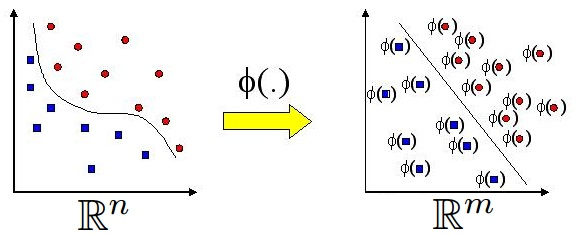
\includegraphics[width=0.4\linewidth]{images/svm-transform-space.jpg}

    \caption{Diagrama de transformación de muestras del espacio vectorial
        $\mathbb{R}^{n}$ a un nuevo espacio $\mathbb{R}^{m}$, con $n \leq m$.}
    \label{fig:ocsvm:svm_transformed_space}
\end{figure}


\subsubsection{Funciones \textit{kernel}}

La transformación de muestras a espacios de mayor dimensión trae consigo
la dificultad de realizar las multiplicaciones de vectores en dichos
espacios. Las multiplicaciones presentes en las ecuaciones
\ref{eq:ocsvm:hyperplane2} y \ref{eq:ocsvm:min_problem_restr2} pueden
provocar que el clasificador consuma demasiados recursos o necesite mucho
tiempo de computación, haciendo que el uso del clasificador en ambientes
reales ya no sea posible
\citep{rieck2009machine}. % from section 3 - kernels (intro paragraph)

Para superar este desafío, se puede emplear unas funciones denominadas
\textit{kernels}, que permiten omitir esas multiplicaciones de vectores
en el nuevo espacio. Los \textit{kernels} comparan dos vectores del
espacio original $\mathbb{R}^{n}$ y retornan un valor escalar que indica
la similitud que dichos vectores presentan en el nuevo espacio
$\mathbb{R}^{m}$ de mayor dimensión.
El resultado producido por estas funciones equivale al producto escalar
de los dos vectores en el nuevo espacio $\mathbb{R}^{m}$, como se
puede observar también en la \autoref{eq:ocsvm:kernel}, pero con la
ventaja de que no se realiza realmente esta multiplicación costosa
\citep{rieck2009machine}. % from section 3.1 - kernels | section 3.2 - geometry

\begin{equation}
    \label{eq:ocsvm:kernel}
    K(\vec{x_{1}}, \vec{x_{2}})
    \ = \
    \phi(\vec{x_{1}}) \cdot \phi(\vec{x_{2}})
\end{equation}

Estos \textit{kernels} no son exclusivos de los clasificadores
\gls{acr3:ocsvm} ni de \gls{acr3:svm}s en general, pero se ha utilizado
estas funciones con mucho éxito en este tipo de clasificadores.
Existen varias opciones de kernels que pueden utilizarse, los más
conocidos son el \textit{kernel} lineal, el polinomial, el sigmoidal
y el \textit{Radial Basis Function} (RBF) \textit{kernel}
\citep{rieck2009machine}. % from section 3.2 - geometry
Usando el \textit{kernel} lineal, el hiperplano separador queda
representado por un hiperplano también en el espacio original; los
otros tres \textit{kernels} mencionados generan superficies no lineales
en el espacio original.
Realizando varias pruebas para comparar la efectividad de estos \textit{kernels},
el \gls{acr3:rbf} es el que arrojó mejores resultados. Además, varios trabajos
relacionados han empleado este \textit{kernel} con éxito para sus tareas
de clasificación, como podemos ver en los trabajos \citep{parhizkar2015oc}
y \citep{perdisci2006using}. Por estos motivos, nosotros utilizamos el
\gls{acr3:rbf} en los clasificadores dentro de nuestro detector
\gls{acr3:name}.
La formulación del \textit{kernel} \gls{acr3:rbf} puede ser expresada
según la \autoref{eq:ocsvm:kernel_rbf}
\citep{parhizkar2015oc}. % from section II.A - one class SVM

\begin{equation}
    \label{eq:ocsvm:kernel_rbf}
    K(\vec{x_{1}}, \vec{x_{2}})
    \ = \
    \phi(\vec{x_{1}}) \cdot \phi(\vec{x_{2}})
    \ = \
    \exp(
        - \gamma \lVert \vec{x_{1}} - \vec{x_{2}} \lVert^2
    )
\end{equation}

En esta ecuación, se puede ver que el \textit{kernel} obtiene el cuadrado
de la norma $l_{2}$ (o distancia euclidiana) de la diferencia de dos
vectores en el espacio original. Este resultado escalar es multiplicado
por un factor $\gamma$, usando este nuevo resultado en una exponenciación
con la base de los logaritmos naturales.
Estas operaciones son computacionalmente más eficientes que la
multiplicación de vectores en espacios de mayores dimensiones
\citep{rieck2009machine}. % from section 3.2 - geometry

En el contexto del \gls{acr3:ocsvm}, el parámetro \gls{sim3:gammai}
determina la dimensión de la región de influencia de cada muestra de
entrenamiento del grupo \gls{sim3:gi}. Esto regula la cercanía necesaria
de nuevas muestras a las muestras de entrenamiento para ser consideradas
pertenecientes a la clase conocida. Este parámetro tiene relación inversa
al radio de la región de influencia de las muestras.
Esto significa que valores menores de \gls{sim3:gammai} aumentan el radio
de la región de influencia de las muestra de entrenamiento, causando que
la superficie separadora que representa al hiperplano en el espacio original
$\mathbb{R}^{n}$ se encuentre más alejada de dichas muestras. En cambio,
valores mayores de \gls{sim3:gammai} reducen este radio de influencia,
permitiendo una superficie más cercana a las muestras vistas.

La \autoref{fig:ocsvm:gamma_values} muestra, con un ejemplo de peticiones
\gls{acr3:http}, la superficie separadora no lineal obtenida en el
espacio original con dos \textit{kernels}. El \gls{acr3:rbf} permite
detectar más anomalías (círculos amarillos) que el \textit{kernel} lineal,
que solamente puede trazar una superficie lineal en el espacio original.
Además, se ilustra la influencia del parámetro \gls{sim3:gammai} en la
forma de la superficie separadora, mostrando que \gls{sim3:gammai} mayor
genera una superficie más ajustada a las muestras de entrenamiento.

\begin{figure}[ht]
    \centering
    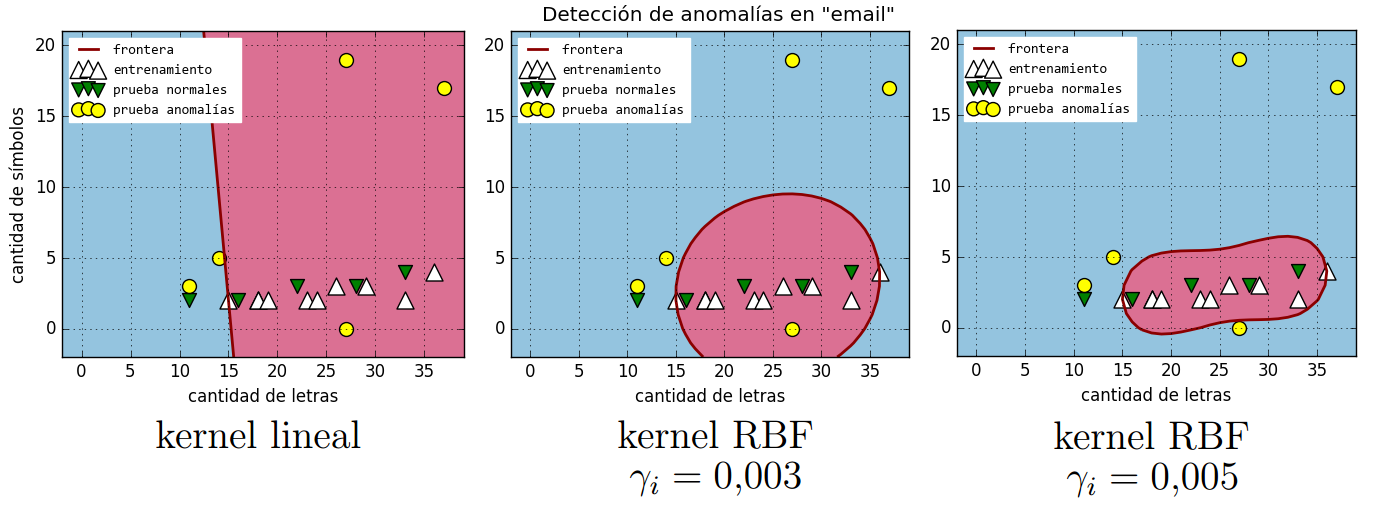
\includegraphics[width=\linewidth]{images/ocsvm-rbf-gamma.png}

    \caption{Comparación de superficies separadoras obtenidas por el
        \gls{acr3:ocsvm} con distintos \textit{kernels} y parámetros.}
    \label{fig:ocsvm:gamma_values}
\end{figure}


\subsubsection{Formulación dual de la optimización}

Para aprovechar la facilidad de cálculo que brindan los \textit{kernels},
es conveniente que el clasificador \gls{acr3:ocsvm} no resuelva directamente
el problema de optimización de la \autoref{eq:ocsvm:min_problem_goal1},
sino que resuelva la formulación dual del problema.
Esta formulación dual queda expresada como se puede observar en la
\autoref{eq:ocsvm:min_problem_dual_goal}, sujeto a las restricciones
que muestra la \autoref{eq:ocsvm:min_problem_dual_restr}
\citep{aggarwal2013outlier}. % from section 3.4 - OCSVM

\begin{equation}
    \label{eq:ocsvm:min_problem_dual_goal}
    \min_{a_{i}}
    \
    \frac{1}{2} \ a_{i} \ S_{i} \ a_{i}^{T}
\end{equation}

\begin{equation}
    \label{eq:ocsvm:min_problem_dual_restr}
    \sum_{j=1}^{\lvert G_{i} \rvert} a_{ij} \ = \ 1
    \ , \quad
    0 \leqslant a_{ij} \leqslant \frac{1}{\nu_{i} \lvert G_{i} \rvert}
    \
    \forall j = 1,2, \dots, \lvert G_{i} \rvert
\end{equation}

En estas ecuaciones, $S_{i}$ es una matriz simétrica que representa los
productos escalares de todas las muestras de entrenamiento multiplicadas
entre ellas en el espacio de dimensiones mayores $\mathbb{R}^{m}$;
ambas dimensiones de esta matriz equivalen a la cantidad de muestras
$\lvert G_{i} \rvert$.
El vector $a_{i}$ contiene una cantidad $\lvert G_{i} \rvert$ de
coeficientes variables que corresponden a cada una de las muestras, y la
formulación dual de la optimización busca encontrar estos coeficientes.
De esta forma, la minimización consta de la multiplicación de un vector
fila $a_{i}$ por una matriz simétrica $S_{i}$, y el vector fila resultante
es multiplicado por el vector columna $a_{i}^{T}$, lo que resulta
finalmente en un valor escalar a ser minimizado.

Las muestras de entrenamiento que tengan coeficiente $a_{ij}$ mayor a
0 serán los vectores de soporte del clasificador. Mayormente, los vectores
de soporte son un subconjunto reducido de las muestras de entrenamiento,
resultando finalmente en un vector $a_{i}$ con la mayoría de los coeficientes
iguales a 0
\citep{perdisci2006using}. % from section 2.1 - OneClassSVM

La matriz simétrica $S_{i}$, que está presente en la formulación dual
de la optimización, representa las multiplicaciones de vectores
que se busca omitir por su alto costo computacional. Esta matriz puede
ser reemplazada por los resultados de un \textit{kernel}. Esto se logra
construyendo una matriz con las mismas dimensiones que $S_{i}$, pero
cuyos elementos son obtenidos mediante un \textit{kernel} en vez de
multiplicación de vectores.

Después de resolver la minimización de la formulación dual, que
presentamos en la \autoref{eq:ocsvm:min_problem_dual_goal}, el clasificador
\gls{acr3:ocsvm} ya tiene disponible el vector de coeficientes $a_{i}$
del grupo \gls{sim3:gi}.
Entonces, el hiperplano definido en la \autoref{eq:ocsvm:hyperplane2}
también puede ser expresado en términos del \textit{kernel} $K_{i}$ que
fue utilizado para sustituir $S_{i}$ en la formulación dual y el vector
$a_{i}$ obtenido por la minimización.

De esta forma, el hiperplano del clasificador puede quedar definido como
lo muestra la \autoref{eq:ocsvm:hyperplane3}
\citep{aggarwal2013outlier}. % from section 3.4 - OCSVM

\begin{equation}
    \label{eq:ocsvm:hyperplane3}
    \vec{w_{i}} \cdot \phi(\vec{x})
    \ - \
    \rho_{i}
    \ = \
    \sum_{j=1}^{\lvert G_{i} \rvert}
    \left(
        a_{ij} \, K_{i}(\vec{f_{ij}}, \vec{x})
    \right)
    \ - \
    \rho_{i}
    \ = \
    0
\end{equation}

Como ya mencionamos, utilizamos el \textit{kernel} \gls{acr3:rbf} en
nuestro \gls{acr3:waf}. Reemplazando la fórmula de este \textit{kernel},
que fue presentada en la \autoref{eq:ocsvm:kernel_rbf}, podemos definir
el hiperplano de la \autoref{eq:ocsvm:hyperplane3} de la forma como lo
expresa la \autoref{eq:ocsvm:hyperplane4}, donde \gls{sim3:gammai} es el
parámetro del \textit{kernel} para el clasificador del grupo \gls{sim3:gi}.

\begin{equation}
    \label{eq:ocsvm:hyperplane4}
    \vec{w_{i}} \cdot \phi(\vec{x})
    \ - \
    \rho_{i}
    \ = \
    \sum_{j=1}^{\lvert G_{i} \rvert}
    \left(
        a_{ij} \,
        \exp(
            - \gamma_{i} \lVert \vec{f_{ij}} - \vec{x} \lVert^2
        )
    \right)
    \ - \
    \rho_{i}
    \ = \
    0
\end{equation}

De esta forma, el clasificador \gls{acr3:ocsvm} puede construir un
hiperplano separador a través de la simulación de multiplicación de
vectores en espacios de altas dimensiones, pero sin incurrir
realmente en los elevados costos computacionales que implicaría la
realización de esas multiplicaciones.


\subsection{Fase de detección}

Después de la fase de entrenamiento, el clasificador \gls{acr3:ocsvm}
está preparado para clasificar nuevas muestras, analizando de que lado
del hiperplano se encuentran las mismas. Si están situadas en el lado
opuesto al origen, serán consideradas como pertenecientes a la clase
conocida. En caso contrario, no pertenecerán a dicha clase
\citep{perdisci2006using}. % from section 2.1 - OneClassSVM
En nuestro contexto de detección de anomalías, el \gls{acr3:waf} representa
cada nueva petición \gls{acr3:http} con un vector de \textit{features}
con dimensiones correspondientes al grupo \gls{sim3:gi} según método y
\gls{acr3:url} de la petición. Luego se analiza la posición de ese vector
con respecto al hiperplano trazado por el clasificador del grupo.

En esta fase de detección, el clasificador \gls{acr3:ocsvm} emplea la
fórmula del hiperplano en una función de decisión con el fin de determinar
si una muestra nueva pertenece a la clase conocida o no. En la
\autoref{eq:ocsvm:decision1} se puede observar la formulación de esta
función de decisión en términos del hiperplano
\citep{amer2013paper}. % from section 3.1 - Motivation of OneClassSVM

\begin{equation}
    \label{eq:ocsvm:decision1}
    g_{i}(\vec{x})
    \ = \
    \begin{cases}
        \vec{w_{i}} \cdot \vec{x} - \rho_{i} \ \geqslant \ 0    & +1 \\
        \text{caso contrario}                                   & -1
    \end{cases}
\end{equation}

En esta ecuación, \gls{sim3:wi} es el vector que define el hiperplano
del grupo, $\vec{x}$ es el vector que representa las nuevas muestras a
analizar, \gls{sim3:rhoi} es la distancia del hiperplano al origen y
$g_{i}(\vec{x})$ es la función de decisión, que recibe el vector $\vec{x}$
como su argumento.
De esta forma, se obtendrá $g_{i}(\vec{x}) = 1$ para las muestras que se
encuentran separadas del origen por el hiperplano, indicando que las mismas
pertenecen a la clase conocida, pero se tendrá $g_{i}(\vec{x}) = -1$ para
las muestras que se encuentren en el mismo lado que el origen, indicando
que estas últimas no pertenecen a dicha clase.

En el contexto de nuestro \gls{acr3:waf}, nuevas peticiones \gls{acr3:http}
serán representadas por vectores de \textit{features} $\vec{x}$, siempre
atendiendo que las dimensiones de esos vectores sean correspondientes a
sus grupo \gls{sim3:gi} respectivos.
La función $g_{i}(\vec{x})$ retorna el valor positivo para peticiones
detectadas como normales (que serán identificadas como muestras negativas)
y devuelve el valor negativo para aquellas peticiones detectadas como
anomalías (que serán identificadas como muestras positivas o ataques).

Para vectores en espacios de dimensiones mayores, esta función de decisión
incorpora las ya mencionadas funciones de transformación $\phi$, y puede
ser expresada de la forma que lo indica la \autoref{eq:ocsvm:decision2}
\citep{amer2013paper}. % from section 3.1 - Motivation of OneClassSVM

\begin{equation}
    \label{eq:ocsvm:decision2}
    g_{i}(\vec{x})
    \ = \
    \begin{cases}
        \vec{w_{i}} \cdot \phi(\vec{x}) - \rho_{i} \ \geqslant \ 0  & +1 \\
        \text{caso contrario}                                       & -1
    \end{cases}
\end{equation}

Empleando las optimizaciones que nos brindan los \textit{kernels}, podemos
sustituir la multiplicación de vectores en esta función. De esta forma,
la función de decisión que expresada según la \autoref{eq:ocsvm:decision3}
\citep{perdisci2006using}. % from section 2.1 - OneClassSVM

\begin{equation}
    \label{eq:ocsvm:decision3}
    g_{i}(\vec{x})
    \ = \
    \begin{cases}
        \sum_{j=1}^{\lvert G_{i} \rvert}
        \left(
            a_{ij} \, K_{i}(\vec{f_{ij}}, \vec{x})
        \right)
        - \rho_{i} \ \geqslant \ 0  & +1 \\
        \text{caso contrario}       & -1
    \end{cases}
\end{equation}

Finalmente, reemplazando en esta ecuación la fórmula del \textit{kernel}
\gls{acr3:rbf}, obtenemos una función según la \autoref{eq:ocsvm:decision4},
donde $\gamma_{i}$ es el parámetro del \textit{kernel} para el
clasificador del grupo \gls{sim3:gi} correspondiente.

\begin{equation}
    \label{eq:ocsvm:decision4}
    g_{i}(\vec{x})
    \ = \
    \begin{cases}
        \sum_{j=1}^{\lvert G_{i} \rvert}
        \left(
            a_{ij} \,
            \exp(
                - \gamma_{i} \lVert \vec{f_{ij}} - \vec{x} \lVert^2
            )
        \right)
        - \rho_{i} \ \geqslant \ 0  & +1 \\
        \text{caso contrario}       & -1
    \end{cases}
\end{equation}

Se puede observar que la función de decisión, que se utiliza para determinar
de que lado del hiperplano cae una nueva muestra, se reduce a calcular
la norma $l_{2}$ entre la muestra nueva y los vectores de soporte (aquellos
con coeficientes $a_{ij}$ mayor a 0). Considerando que suele haber una
cantidad reducida de vectores de soporte en un clasificador entrenado,
esta función de decisión $g_{i}(\vec{x})$ resulta en computaciones rápidas
y eficientes \citep{perdisci2006using}. % from section 2.1 - OneClassSVM
De esta manera mostramos que el clasificador \gls{acr3:ocsvm} es una
herramienta con un bajo costo computacional durante la fase de detección,
y por lo tanto puede ser empleado en nuestro detector \gls{acr3:name}
para realizar la detección en tiempo real de mensajes \gls{acr3:http}
anómalos.


\section{Trabajos relacionados con One-Class SVM}

En la sección anterior describimos el funcionamiento del clasificador
\gls{acr3:ocsvm}, mostrando las ecuaciones que definen su comportamiento
durante las fases de entrenamiento y detección.
A continuación presentamos algunos trabajos relacionados del área de
\gls{acr3:ids} que utilizan este clasificador.

En \citep{nguyen2016pocad} se presenta un detector llamado \textit{POCAD}.
Este detector extrae conjuntos de \textit{n-grams} de \textit{bytes} de
paquetes \gls{acr3:ip} y peticiones \gls{acr3:http} y luego aplica un
proceso de \textit{clustering} para reducir la cantidad de \textit{features};
\gls{acr3:name} utiliza los procesos de extracción de \textit{features}
presentados en el \autoref{chap:p3_concepts_features}, que no incluyen
\textit{n-grams}.
Posteriormente, \textit{POCAD} utiliza un \gls{acr3:ocsvm} para realizar
la detección de anomalías, de manera similar a nuestra implementación.
Los autores realizan pruebas comparativos con otros sistemas de detección,
concluyendo que su implementación logra una mejor detección que los demás.

En \citep{parhizkar2015oc} se presenta un detector de anomalías llamado
\textit{OC-WAD} para peticiones \gls{acr3:http}. Los autores extraen
una cantidad fija de \textit{features} de las peticiones, a diferencia
de nuestros procesos de extracción que producen una cantidad variable
de \textit{features} que depende de los parámetros presentes en las
peticiones.
Posteriormente, \textit{OC-WAD} utiliza un conjunto de \gls{acr3:ocsvm}
con \textit{kernel} \gls{acr3:rbf} para realizar la detección, poniendo
énfasis en la creación y optimización del conjunto de clasificadores
mediante un algoritmo de enjambres llamado \textit{BeeSnips}.
Nuestro \gls{acr3:name} utiliza también el mismo \textit{kernel} y
clasificador, pero se entrena un clasificador por grupo de método y
\gls{acr3:url}.
Los autores concluyen mediante algunas comparaciones que su implementación
supera algunos otros trabajos que mencionan.

En \citep{perdisci2006using} presentan un detector que extrae conjuntos
de \textit{n-grams} de \textit{bytes} de peticiones \gls{acr3:http}.
También se aplica un proceso de \textit{clustering} sobre los \textit{features}
extraídos. Como ya explicamos, nuestros procesos de extracción no analizan
\textit{n-grams}.
Los autores emplean un conjunto de \gls{acr3:ocsvm} con el \textit{kernel}
\gls{acr3:rbf}; cada uno de los clasificadores es entrenado sobre distintos
subconjuntos de \textit{features}. En cambio, \gls{acr3:name} utiliza
también el mismo \textit{kernel} y clasificador, pero se entrena un
clasificador por grupo de método y \gls{acr3:url}.
Las conclusiones de los autores subrayan la robustez de su detector
frente a ataques que tratan de ocultar su firma utilizando diversas
técnicas de ofuscación.

En \citep{tran2004one} se presenta un detector de anomalías llamado
\textit{OTAD} para analizar paquetes \gls{acr3:ip}. Los autores utilizan
una cantidad fija de cinco \textit{features} que corresponden a datos
obtenidos mediante la herramienta \textit{tcpstat}; nuestra implementación
extrae una cantidad variable de \textit{features} de peticiones
\gls{acr3:http}.
Posteriormente, \textit{OTAD} emplea un clasificador \gls{acr3:ocsvm}
con el \textit{kernel} \gls{acr3:rbf}, utilizando un algoritmo genético
para la optimización de la selección de parámetros. En cambio, \gls{acr3:name}
utiliza también el mismo \textit{kernel} y clasificador, pero sin mecanismo
para la selección automática de parámetros.
Los autores concluyen que su detector obtiene buenos resultados, con la
ventaja de poder utilizar directamente los datos del \textit{tcpstat}
sin necesidad de conversiones o transformaciones.

En \citep{rieck2009machine} se propone un detector de anomalías que trabaja
sobre un conjunto variado de \textit{features} de peticiones \gls{acr3:http},
incluyendo secuencias y árboles para representar relaciones en los datos.
Emplea un tipo de \gls{acr3:ocsvm} que esta implementado de forma distinta
a lo que presentamos en este capítulo; el autor usa un clasificador que
emplea una hiperesfera en vez de un hiperplano para clasificar las muestras.
Concluye que el detector presentado detecta una gran variedad de ataques,
resaltando la baja tasa de falsos positivos.

El éxito en la detección de anomalías que reportan estos trabajos nos
confirma que el clasificador \gls{acr3:ocsvm} es una herramienta útil
para nuestro \gls{acr3:waf}.


\section{Clasificación de peticiones de ejemplo}

Después de haber explicado el funcionamiento del clasificador \gls{acr3:ocsvm},
a continuación ilustramos el proceso de clasificación y detección de
anomalías \gls{acr3:http} que realiza nuestro detector \gls{acr3:name}.
En el \autoref{chap:p3_concepts_features} hemos introducido un ejemplo
mediante el cual explicamos nuestros procesos de extracción de \textit{features}.
En la \autoref{tbl:fe:example_1} se pudo observar 20 peticiones de ejemplo,
con las cuales realizamos la extracción y el escalamiento de los
\textit{features}. Los números finales que representan las peticiones
fueron presentados en las tablas \ref{tbl:fe:example_scaled_whole_req},
\ref{tbl:fe:example_scaled_email} y \ref{tbl:fe:example_scaled_full}.

Para el proceso de clasificación, entrenamos un \gls{acr3:ocsvm} con la
matriz \gls{sim3:mi} obtenida a partir de nuestras peticiones de ejemplo,
la cual tiene 10 filas y 30 columnas.
Para la selección de los valores para \gls{sim3:nui} y \gls{sim3:gammai}
realizamos el entrenamiento con varios valores en el rango
$[\num{0.0001} ; \num{0.5}]$, seleccionando los valores con los mejores
resultados en la fase de detección. De esta forma, para este ejemplo
utilizamos los valores \num{0.2778} y \num{0.0001} para \gls{sim3:nui}
y \gls{sim3:gammai} respectivamente.

\begin{table}[ht]
    \centering
    \small
    \begin{tabularx}{\linewidth}{|c|C|C|C|C|C|}
        \hline
        ID & Grupo         & Vector de soporte & Clasificación real & Clasificación obtenida & Correctamente clasificado \\ \specialrule{1.5pt}{0}{0}
         1 & entrenamiento & -                 & normal             & normal                 & Sí                        \\ \hline
         2 & entrenamiento & -                 & normal             & normal                 & Sí                        \\ \hline
         3 & entrenamiento & -                 & normal             & normal                 & Sí                        \\ \hline
         4 & entrenamiento & -                 & normal             & normal                 & Sí                        \\ \hline
         5 & entrenamiento & Sí                & normal             & normal                 & Sí                        \\ \hline
         6 & entrenamiento & -                 & normal             & normal                 & Sí                        \\ \hline
         7 & entrenamiento & Sí                & normal             & normal                 & Sí                        \\ \hline
         8 & entrenamiento & Sí                & normal             & normal                 & Sí                        \\ \hline
         9 & entrenamiento & Sí                & normal             & normal                 & Sí                        \\ \hline
        10 & entrenamiento & -                 & normal             & normal                 & Sí                        \\ \hline
        11 & detección     & -                 & normal             & normal                 & Sí                        \\ \hline
        12 & detección     & -                 & normal             & normal                 & Sí                        \\ \hline
        13 & detección     & -                 & normal             & anomalía               & -                         \\ \hline
        14 & detección     & -                 & normal             & anomalía               & -                         \\ \hline
        15 & detección     & -                 & normal             & normal                 & Sí                        \\ \hline
        16 & detección     & -                 & anomalía           & anomalía               & Sí                        \\ \hline
        17 & detección     & -                 & anomalía           & anomalía               & Sí                        \\ \hline
        18 & detección     & -                 & anomalía           & anomalía               & Sí                        \\ \hline
        19 & detección     & -                 & anomalía           & anomalía               & Sí                        \\ \hline
        20 & detección     & -                 & anomalía           & anomalía               & Sí                        \\ \hline
    \end{tabularx}

    \caption{Resultados de clasificación de nuestras 20 peticiones de
        ejemplo.}
    \label{tbl:ocsvm:example}
\end{table}

En la \autoref{tbl:ocsvm:example} se pueden observar los resultados del
entrenamiento y la posterior detección de todas las peticiones de ejemplo.
Se puede notar que, como se ha explicado en este capítulo, solamente
algunas de las muestras de entrenamiento (que son las primeras 10 peticiones)
son utilizados como vectores de soporte del clasificador.
Además, la tabla muestra que 18 de las 20 peticiones fueron clasificadas
correctamente por el \gls{acr3:ocsvm} entrenado; solamente dos peticiones
normales fueron categorizadas incorrectamente, mientras que las cinco
anomalías del conjunto de ejemplo fueron detectadas por el clasificador.

Como muestran los resultados, la clasificación no siempre es exitosa,
ya que depende de las muestras con las que debe trabajar el clasificador.
No podemos visualizar en dos o tres dimensiones el espacio original de
30 \textit{features}, ni mucho menos el espacio de dimensiones superiores.
De esta forma, no hemos logrado analizar la superficie separadora que
representa al hiperplano en el espacio original; el análisis de las
componentes principales (PCA) tampoco pudo brindar aportes en este análisis.
La idea de este ejemplo es también resaltar esta realidad en las tareas
de detección de anomalías, mostrando una situación en la cual no se logra
la detección correcta de todas las muestras.

\begin{figure}[ht]
    \centering
    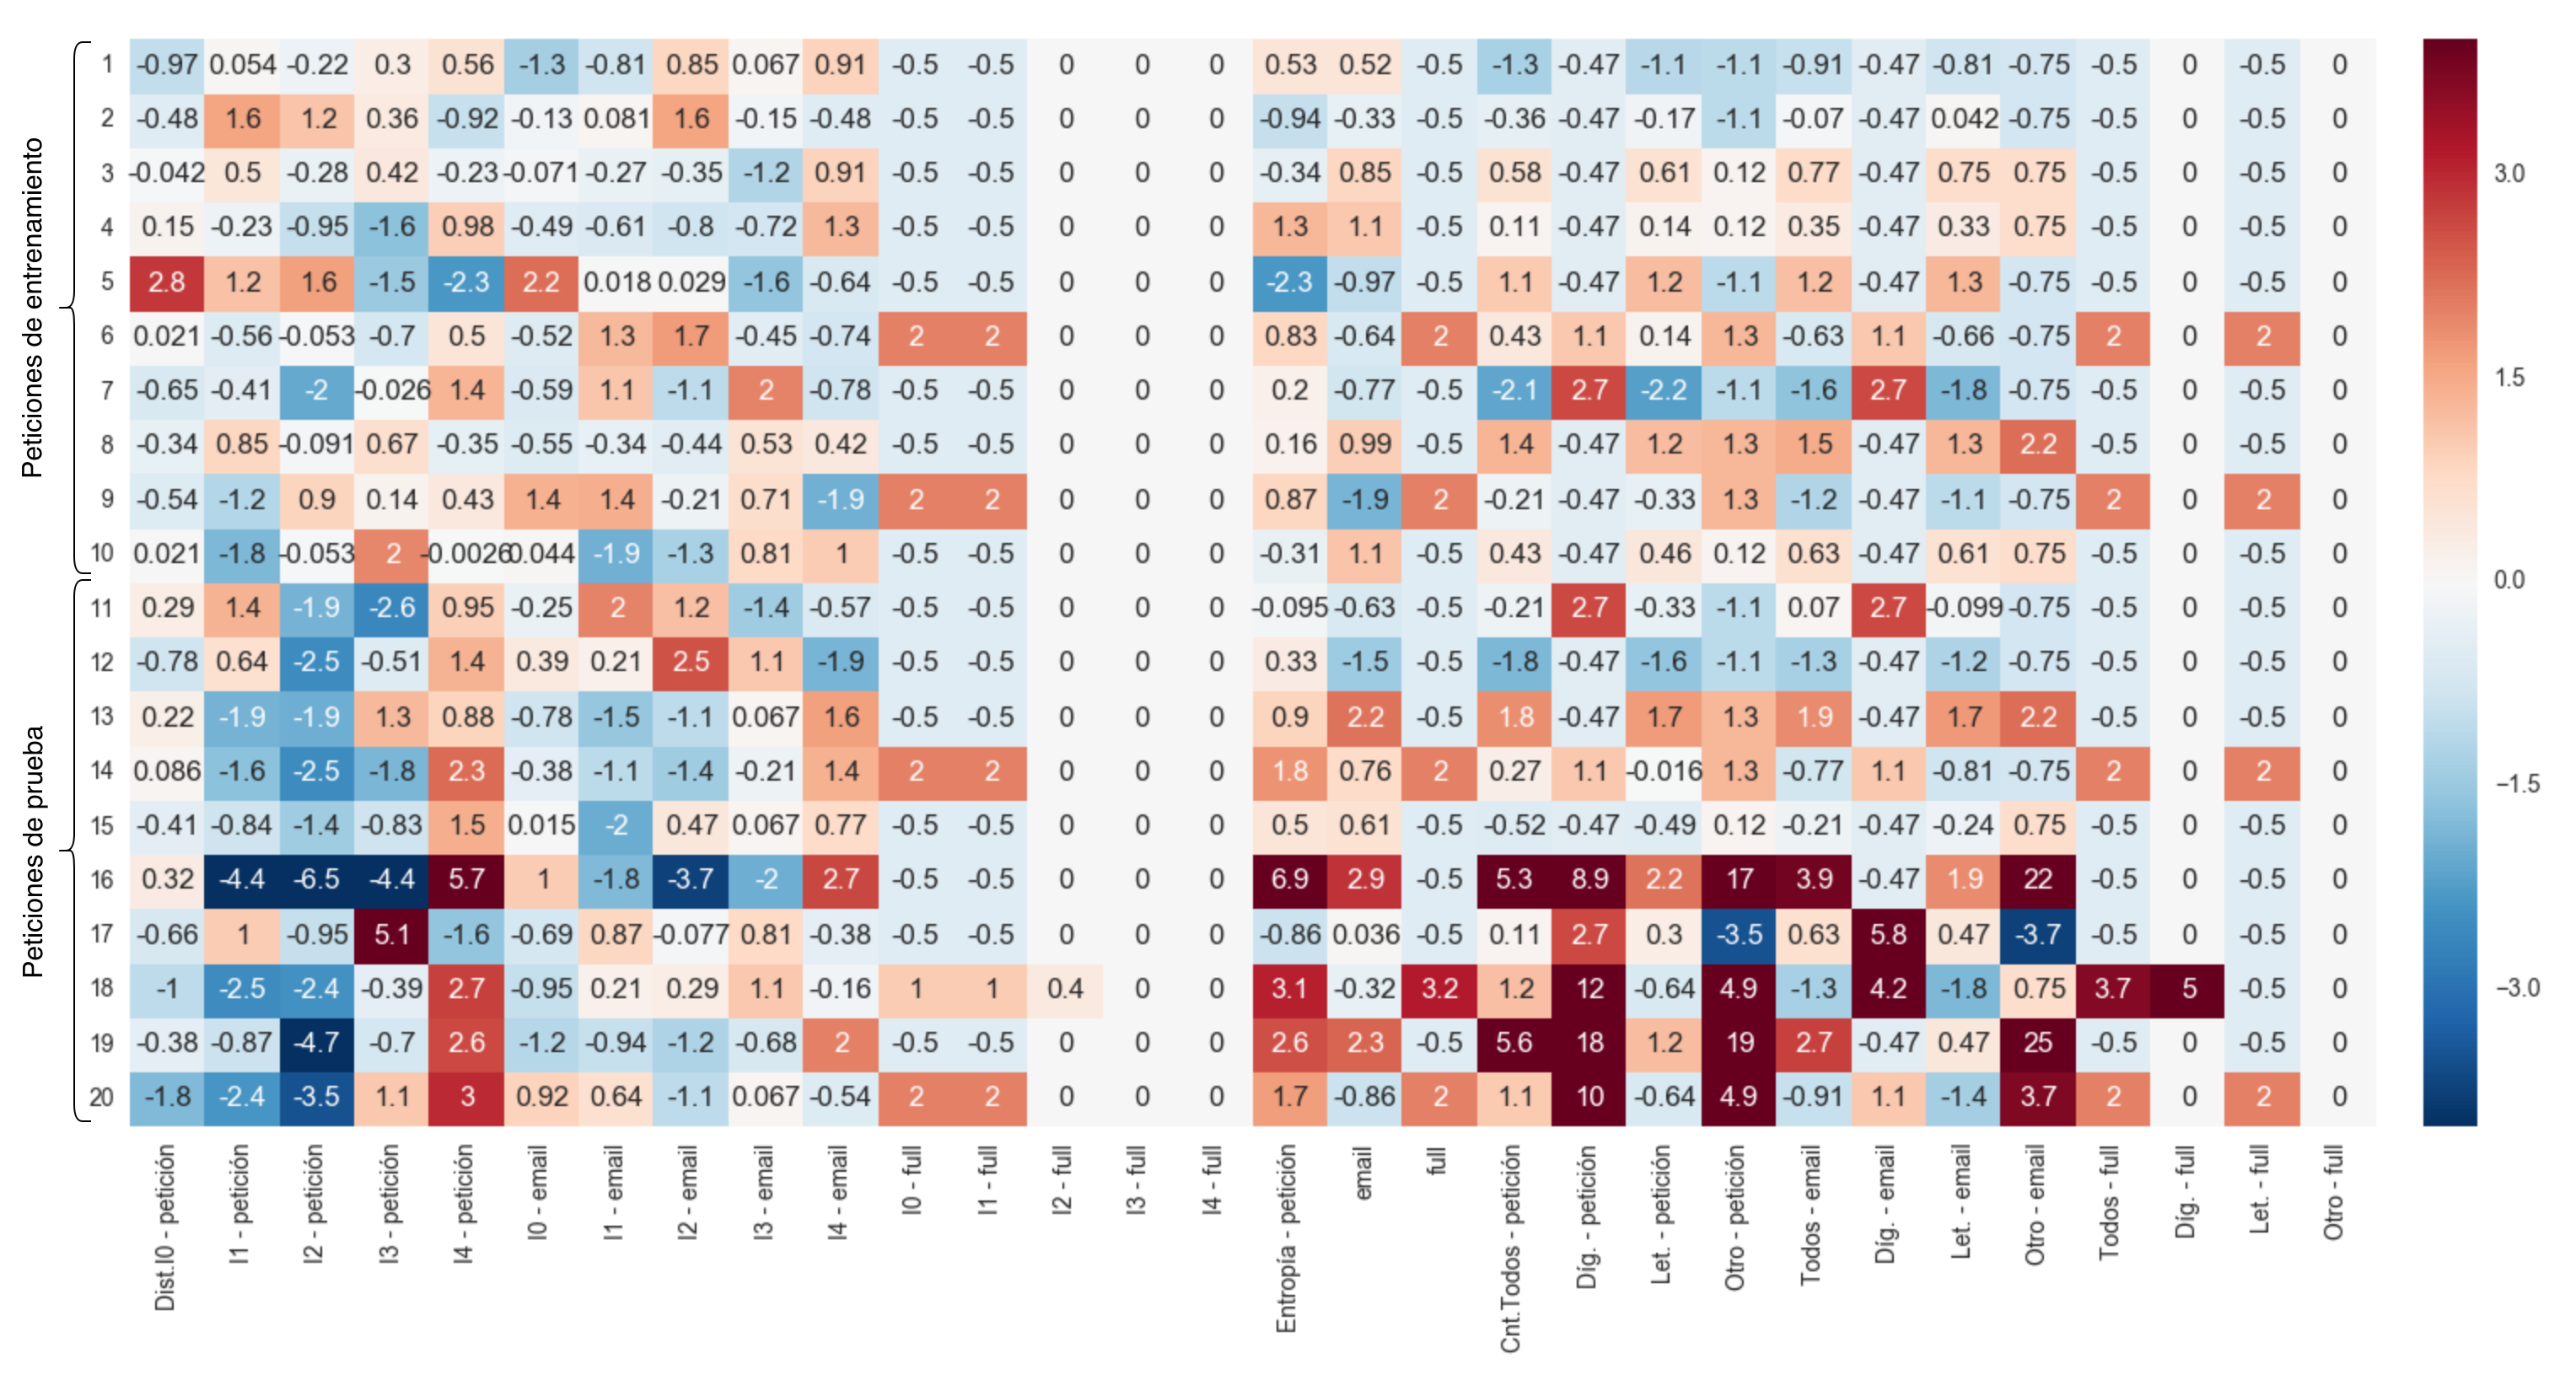
\includegraphics[width=\linewidth]{images/example-features-heatmap.png}

    \caption{Mapa de calor de los \textit{features} extraídos de nuestras
        20 peticiones de ejemplo.}
    \label{fig:ocsvm:example_heatmap}
\end{figure}

En la \autoref{fig:ocsvm:example_heatmap} se puede observar los números
escalados de todos nuestros \textit{features} para las 20 peticiones de
ejemplo, desplegadas dentro de un gráfico del tipo mapa de calor
(\textit{heatmap}) para permitir una mejor visualización de los rangos
de valores. Cada \textit{features} fue escalado para que su promedio sea 0,
que en el gráfico corresponde al color blanco; regiones de colores rojo o
azul oscuros indican mayor alejamiento del 0.
Se puede notar, por ejemplo, que las peticiones 16 al 20, que contienen
anomalías, tienen mayores ocurrencias de colores oscuros que indican que
esos \textit{features} están alejados del promedio; esto le permite al
\gls{acr3:ocsvm} detectar estas anomalías.

En cambio, la petición 14 tiene un valor mucho más elevado para el último
intervalo de la distribución de caracteres de la petición completa
(quinta columna desde la izquierda) que todas las peticiones de entrenamiento,
lo que pudo haber provocado que el clasificador no detectó esa petición
como normal. Lo mismo se da para la petición 13, que tiene una entropía
del parámetro \textit{email} más elevada que las peticiones de entrenamiento.

Esta representación de los \textit{features} puede ser de utilidad para
continuar el análisis de los datos, inspeccionando las relaciones entre
los \textit{features} extraídos y los resultados de clasificación
mostrados en la \autoref{tbl:ocsvm:example}.

    \renewcommand{\newCommandChapterTitle}{Implementación de OCS-WAF}
\chapter{\newCommandChapterTitle}
\markright{\hfill \thechapter. \newCommandChapterTitle}
\label{chap:p3_new_waf}


Este capítulo presenta los detalles de implementación de \gls{acr3:name},
un \gls{acr3:waf} que utiliza los componentes descritos en los capítulos
anteriores para la detección de mensajes \gls{acr3:http} anómalos.
Iniciaremos este capítulo explicando algunos conceptos sobre \gls{acr3:waf}s
y detección de anomalías, luego presentamos la arquitectura general de
nuestra implementación y después describimos el funcionamiento de la misma
durante las fases de entrenamiento y detección, detallando los pasos
intermedios presentes en cada una de las dos fases.

El código fuente de nuestra implementación está disponible en nuestro
repositorio público bajo la dirección \TheRepoUrl.


\section{Detección de intrusiones con \textit{Web Application Firewalls}}

Los sistemas de detección de intrusión (\gls{acr3:ids} -
\textit{Intrusion Detection System}) son programas o dispositivos
especializados para monitorear las actividades en un sistema en busca
de intrusiones no autorizadas o posibles ataques, siendo un elemento
fundamental y necesario para garantizar la seguridad del sistema
\citep{scarfone2007guide}. % from section 2 - IDS and IPS principles

Se pueden utilizar tres criterios principales para clasificar los
\gls{acr3:ids}, en primer lugar según los modos de respuesta que utilizan
frente a intrusiones, en segundo lugar según las fuentes de datos que
emplean para sus análisis y en tercer lugar se los puede clasificar según
la metodología de detección que usan
\citep{torranoGimenez2015study}. % from section 2.2.1 - IDS classification
A continuación damos una breve explicación de los \gls{acr3:ids} según
cada uno de estos criterios de clasificación, resaltando las características
más relevantes de cada caso.

\begin{itemize}
    \item
    De acuerdo al modo de respuesta del sistema, se puede tener:

    \begin{itemize}
        \item
        \textit{Intrusion Detection System} (\gls{acr3:ids}):
        esta clase de sistema actúa de forma pasiva y solamente lanza
        alertas o mensajes cuando detecta actividades no autorizadas,
        pero no realiza acciones de contención.

        \item
        \textit{Intrusion Prevention System} (\gls{acr3:ips}):
        este tipo de sistema trabaja de forma activa para prevenir
        intrusiones y está equipado con herramientas para mitigar los
        daños de posibles ataques.
    \end{itemize}

    \item
    De acuerdo a las fuentes de datos para el análisis, se puede tener:

    \begin{itemize}
        \item
        \textit{Host-based systems} (\gls{acr3:hids}):
        esta clase de sistema analiza las actividades de máquinas
        individuales, monitoreando diferentes aspectos de las mismas,
        como por ejemplo las aplicaciones abiertas, los procesos en
        ejecución, los accesos y las modificaciones de archivos, entre
        otros.

        \item
        \textit{Network-based systems} (\gls{acr3:nids}):
        este tipo de sistema analiza el tráfico que pasa por las redes
        de comunicación, monitoreando a nivel de paquetes \gls{acr3:ip}
        o también a nivel de mensajes \gls{acr3:http}.
        Normalmente, estos sistemas son colocados en puntos de entrada a
        una red, o frente a sistemas críticos, como por ejemplo servidores.
        En el caso de que se analicen mensajes \gls{acr3:http} se puede
        hablar específicamente de cortafuegos para aplicaciones web
        (\gls{acr3:waf} - \textit{Web Application Firewall}).
    \end{itemize}

    \item
    De acuerdo a la metodología de detección, se puede tener:

    \begin{itemize}
        \item
        \textit{Signature-based detection}:
        esta clase de sistemas busca patrones de ataques a partir de
        una lista de firmas de ataques conocidos.

        \item
        \textit{Anomaly-based detection}:
        este tipo de sistemas busca desviaciones del comportamiento
        normal o anomalías en las fuentes de datos que monitorea, ya
        que estas anomalías pueden indicar intrusiones o ataques.

        \item
        \textit{Hybrid systems}:
        se puede combinar también los sistemas de detección por firmas
        y anomalías, para tratar de aprovechar las ventajas que provee
        cada uno.
    \end{itemize}
\end{itemize}

Considerando estos conceptos expuestos, según el modo de respuesta
que pueden tener los sistemas, nuestra implementación es un \gls{acr3:ips}
por poseer mecanismos para bloquear mensajes anómalos; esos bloqueos
pueden ser desactivadas para utilizar solamente detección pasiva.
Por otro lado, como nuestra implementación utiliza mensajes \gls{acr3:http}
como su fuente de datos para el análisis, \gls{acr3:name} puede ser
considerado un sistema \gls{acr3:nids}.

En tercer lugar, considerando la metodología de detección, \gls{acr3:name}
utiliza \textit{anomaly-based detection}, ya que este método tiene
ventajas sobre la detección por firmas.
Para que un \gls{acr3:waf} pueda utilizar eficazmente el método por
firmas, es necesario que el mismo mantenga una lista actualizada de
las firmas de los ataques conocidos. La lista de firmas de ataques
descubiertos crece constantemente y probablemente nunca deje de crecer.
Durante el análisis de los mensajes, el \gls{acr3:waf} debe tomar en
consideración toda la lista de firmas en busca de ataques, y esta lista
creciente causa que aumente el tiempo de procesamiento y el uso de
recursos para este proceso de detección
\citep{kruegel2003anomaly}. % from section 1 - introduction

El método de detección de anomalías no requiere una lista de firmas,
sino que trabaja en dos fases: entrenamiento y detección. En la fase
de entrenamiento, este tipo de \gls{acr3:waf} construye modelos que
representan a los mensajes \gls{acr3:http} normales. Se basa en la premisa
de que los ataques se diferencian en alguna forma de los mensajes normales.
Así, durante la fase de detección o monitoreo, este tipo de \gls{acr3:waf}
compara los mensajes nuevos con los modelos construidos anteriormente,
con el fin de detectar desviaciones significativas, es decir, para detectar
aquellos mensajes \gls{acr3:http} que son considerados anomalías con
respecto a los mensajes normales vistos durante entrenamiento
\citep{kruegel2003anomaly}. % from section 1 - introduction

Para \gls{acr3:waf}s basados en anomalías, la fase de entrenamiento es
obligatoria una vez al inicio del uso y después solamente si existen
cambios en los mensajes normales, por ejemplo después de una modificación
a una de las aplicaciones web protegidas por el \gls{acr3:waf} en cuestión.
El método de detección por anomalías tiene la ventaja de poder detectar
anomalías debidas a nuevos tipos de ataques desde el momento que aparezcan,
mientras que los métodos por firmas dependen de la actualización de su
lista de ataques conocidos
\citep{kruegel2003anomaly}. % from section 1 - introduction


\section{Arquitectura de nuestra implementación}

El detector \gls{acr3:name}, implementado en el marco de este trabajo,
consiste en un \textit{proxy} \gls{acr3:http} que contiene herramientas
para el análisis de las peticiones que pasan por el mismo.
Este \gls{acr3:waf} es colocado frente a las aplicaciones web a ser
protegidas, de forma que todo el tráfico entrante y saliente de dichas
aplicaciones pase por este dispositivo de detección. La arquitectura
general de \gls{acr3:name} se puede observar en la
\autoref{fig:waf:waf_diagram_overview}.

Se puede observar dos fases diferentes en \gls{acr3:name}, una de
entrenamiento y otra de detección. La fase de entrenamiento es un proceso
en el cual se utilizan peticiones \gls{acr3:http} recolectadas que
representan el tráfico normal de las aplicaciones web para entrenar
los \gls{acr3:ocsvm} (un clasificador por grupo de peticiones).
En la fase de detección, \gls{acr3:name} analiza nuevas peticiones
entrantes mediante los clasificadores entrenados con el fin de determinar
si dichas peticiones son normales (muestras de la clase conocida) o
anómalas (muestras positivas o ataques).
Ambas fases incluyen un paso de preprocesamiento, que consiste en una
extracción de \textit{features} para representar las peticiones con
vectores numéricos.
En las siguientes secciones de este capítulo presentamos los pasos
intermedios que componen cada fase.

\gls{acr3:name} es una implementación sencilla hecha en el lenguaje
de programación \textit{Python} en su versión 3.5.
La base está compuesta por un \textit{proxy} \gls{acr3:http} creado por
Philippe Lagadec \citep{cherryproxy2011}. Fueron realizadas algunas
modificaciones a esta base de forma que funcione con nuestra versión de
\textit{Python}, ya que originalmente fue escrito para \textit{Python} 2.
Esta base realiza todas las tareas de recibir las peticiones \gls{acr3:http}
y enviarlas a las aplicaciones web destino, como también realiza el proceso
inverso para hacer llegar las respuestas de las aplicaciones de vuelta
al origen de las peticiones. Además, la base provee una simple interfaz
de funciones que fueron extendidas para realizar el análisis de las
peticiones.
\gls{acr3:name} solamente analiza las peticiones entrantes, lo que se puede
observar también en la \autoref{fig:waf:waf_diagram_overview}, pero nuestra
implementación puede ser extendida para incluir el análisis de las respuestas
que son retornadas por las aplicaciones protegidas.
Dentro de nuestro repositorio, la base modificada en cuestión se encuentra en
los archivos \path{/waf/proxy_base.py} y también \path{/waf/proxy_implementation.py},
mientras que nuestros procesos de extracción de \textit{features} están
en los archivos del directorio \path{/waf/feature_extraction/}.

\begin{figure}[ht]
    \centering
    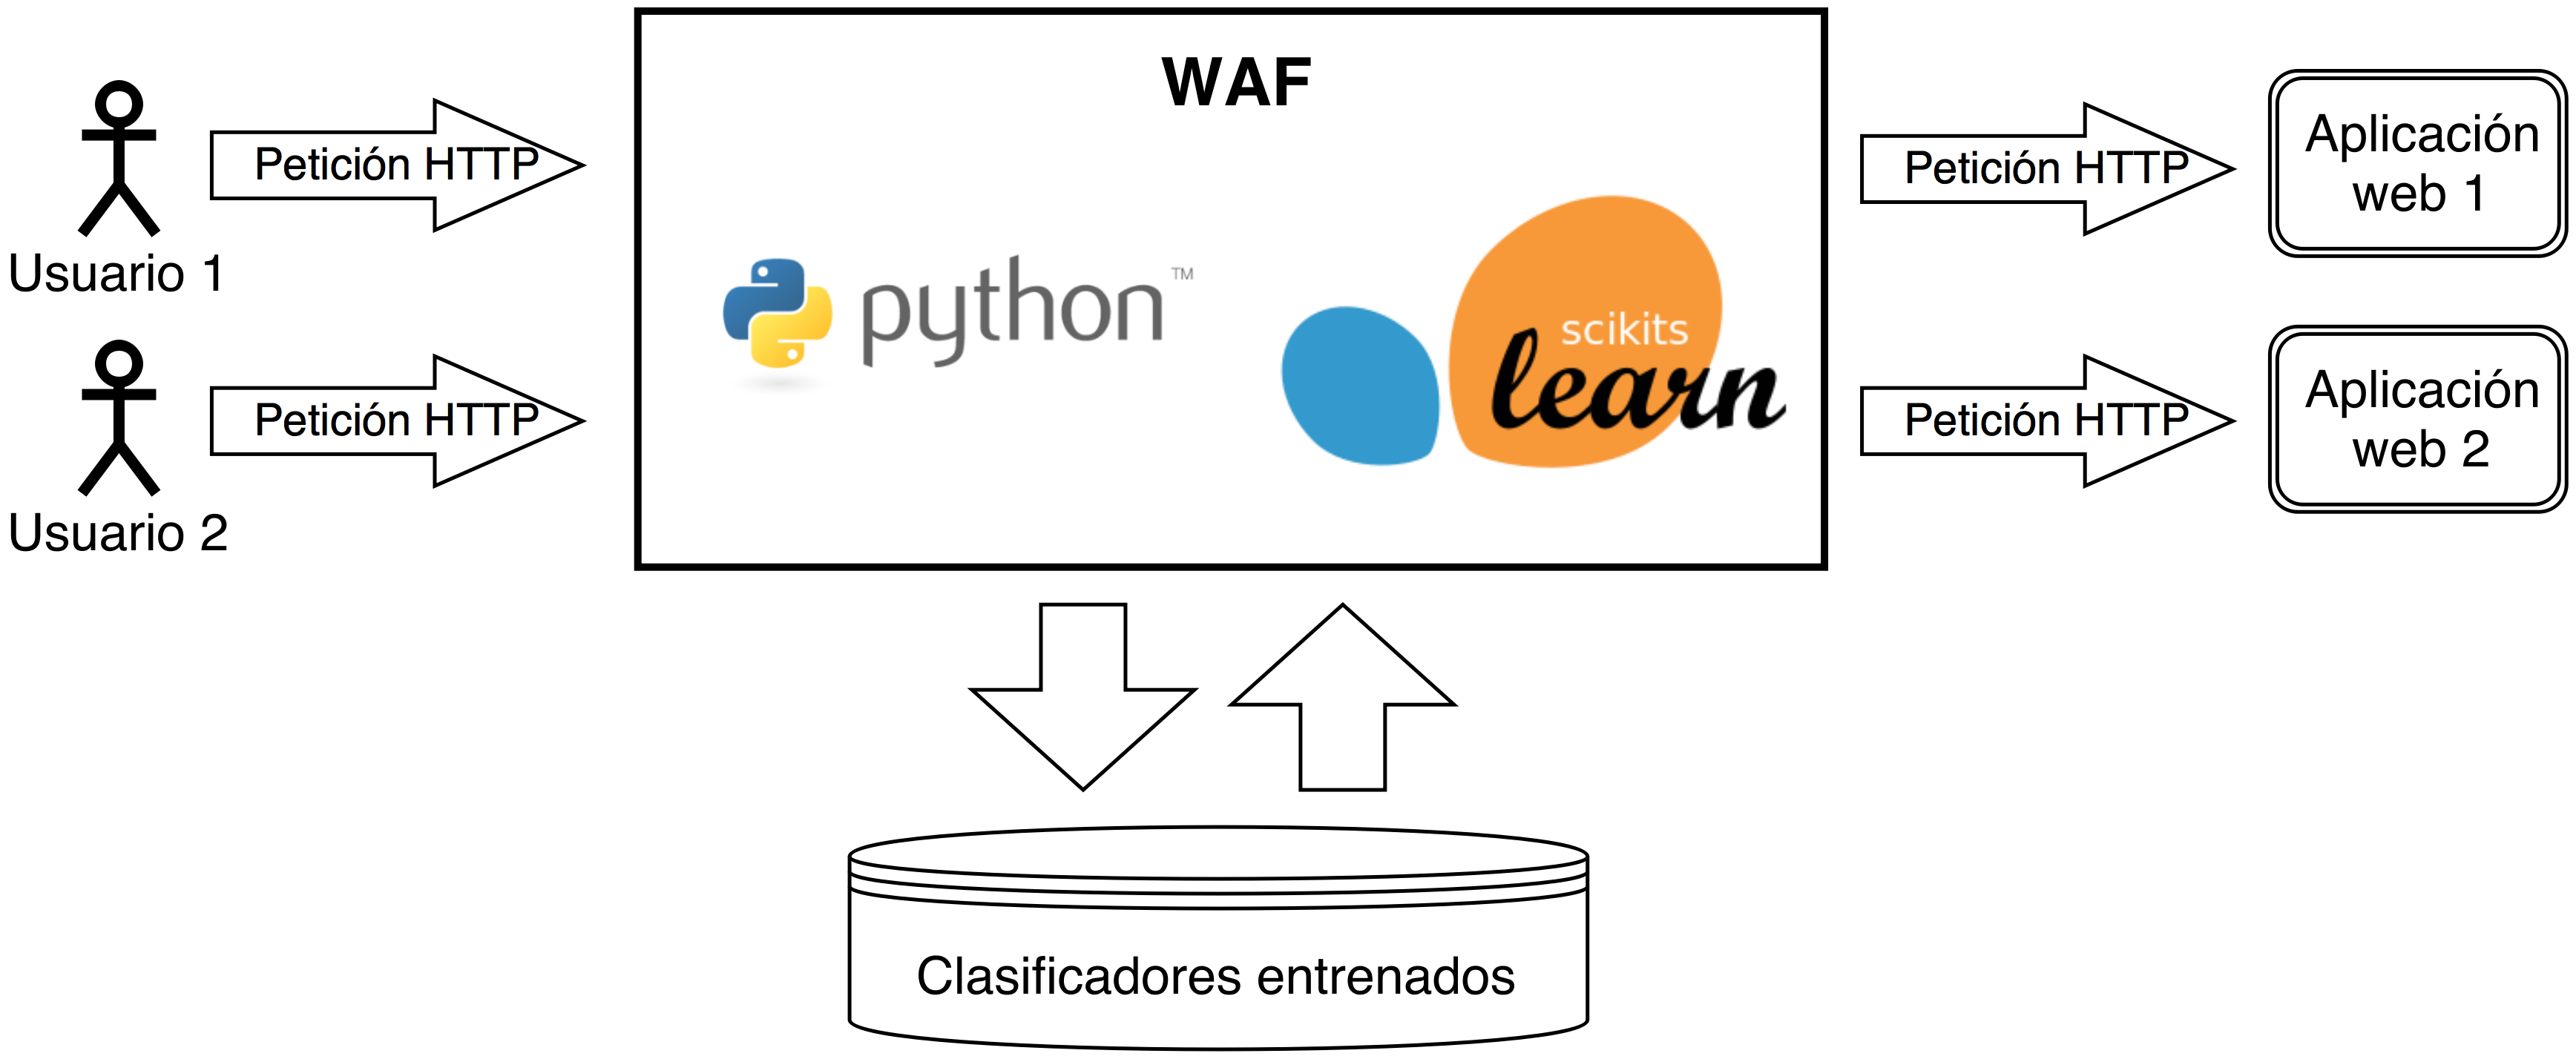
\includegraphics[width=\linewidth]{images/waf-diagram-overview.png}

    \caption{Arquitectura general del funcionamiento de \gls{acr3:name}.}
    \label{fig:waf:waf_diagram_overview}
\end{figure}

\gls{acr3:name} también utiliza la librería \textit{scikit-learn}
\citep{scikit-learn}, que es una librería con herramientas del área de
\gls{acr3:ml} para \textit{Python}. De esta librería se utilizaron varias
herramientas, como por ejemplo, el \textit{BaseEstimator} para implementar
las funciones de extracción de \textit{features}, el \textit{StandardScaler}
para el escalamiento de \textit{features}, el \textit{OneClassSVM} para
el proceso de clasificación y finalmente se emplea el \textit{FeatureUnion}
y el \textit{Pipeline} para coordinar el flujo de datos entre todos estos
componentes.


\section{Fase de entrenamiento}

Esta fase sirve para preparar el \gls{acr3:name} para la detección de
peticiones \gls{acr3:http} anómalas. La \autoref{fig:waf:waf_diagram_training}
muestra la arquitectura de \gls{acr3:name} en esta fase de entrenamiento.
Se utiliza peticiones recolectadas que representan el tráfico normal de
las aplicaciones web, las cuales pasan por tres pasos intermedios durante
esta fase; primeramente se agrupan las peticiones según su método
\gls{acr3:http} y \gls{acr3:url}, luego se realiza el preprocesamiento
de las peticiones y finalmente se entrena los clasificadores dentro de
cada grupo.

\begin{figure}[ht]
    \centering
    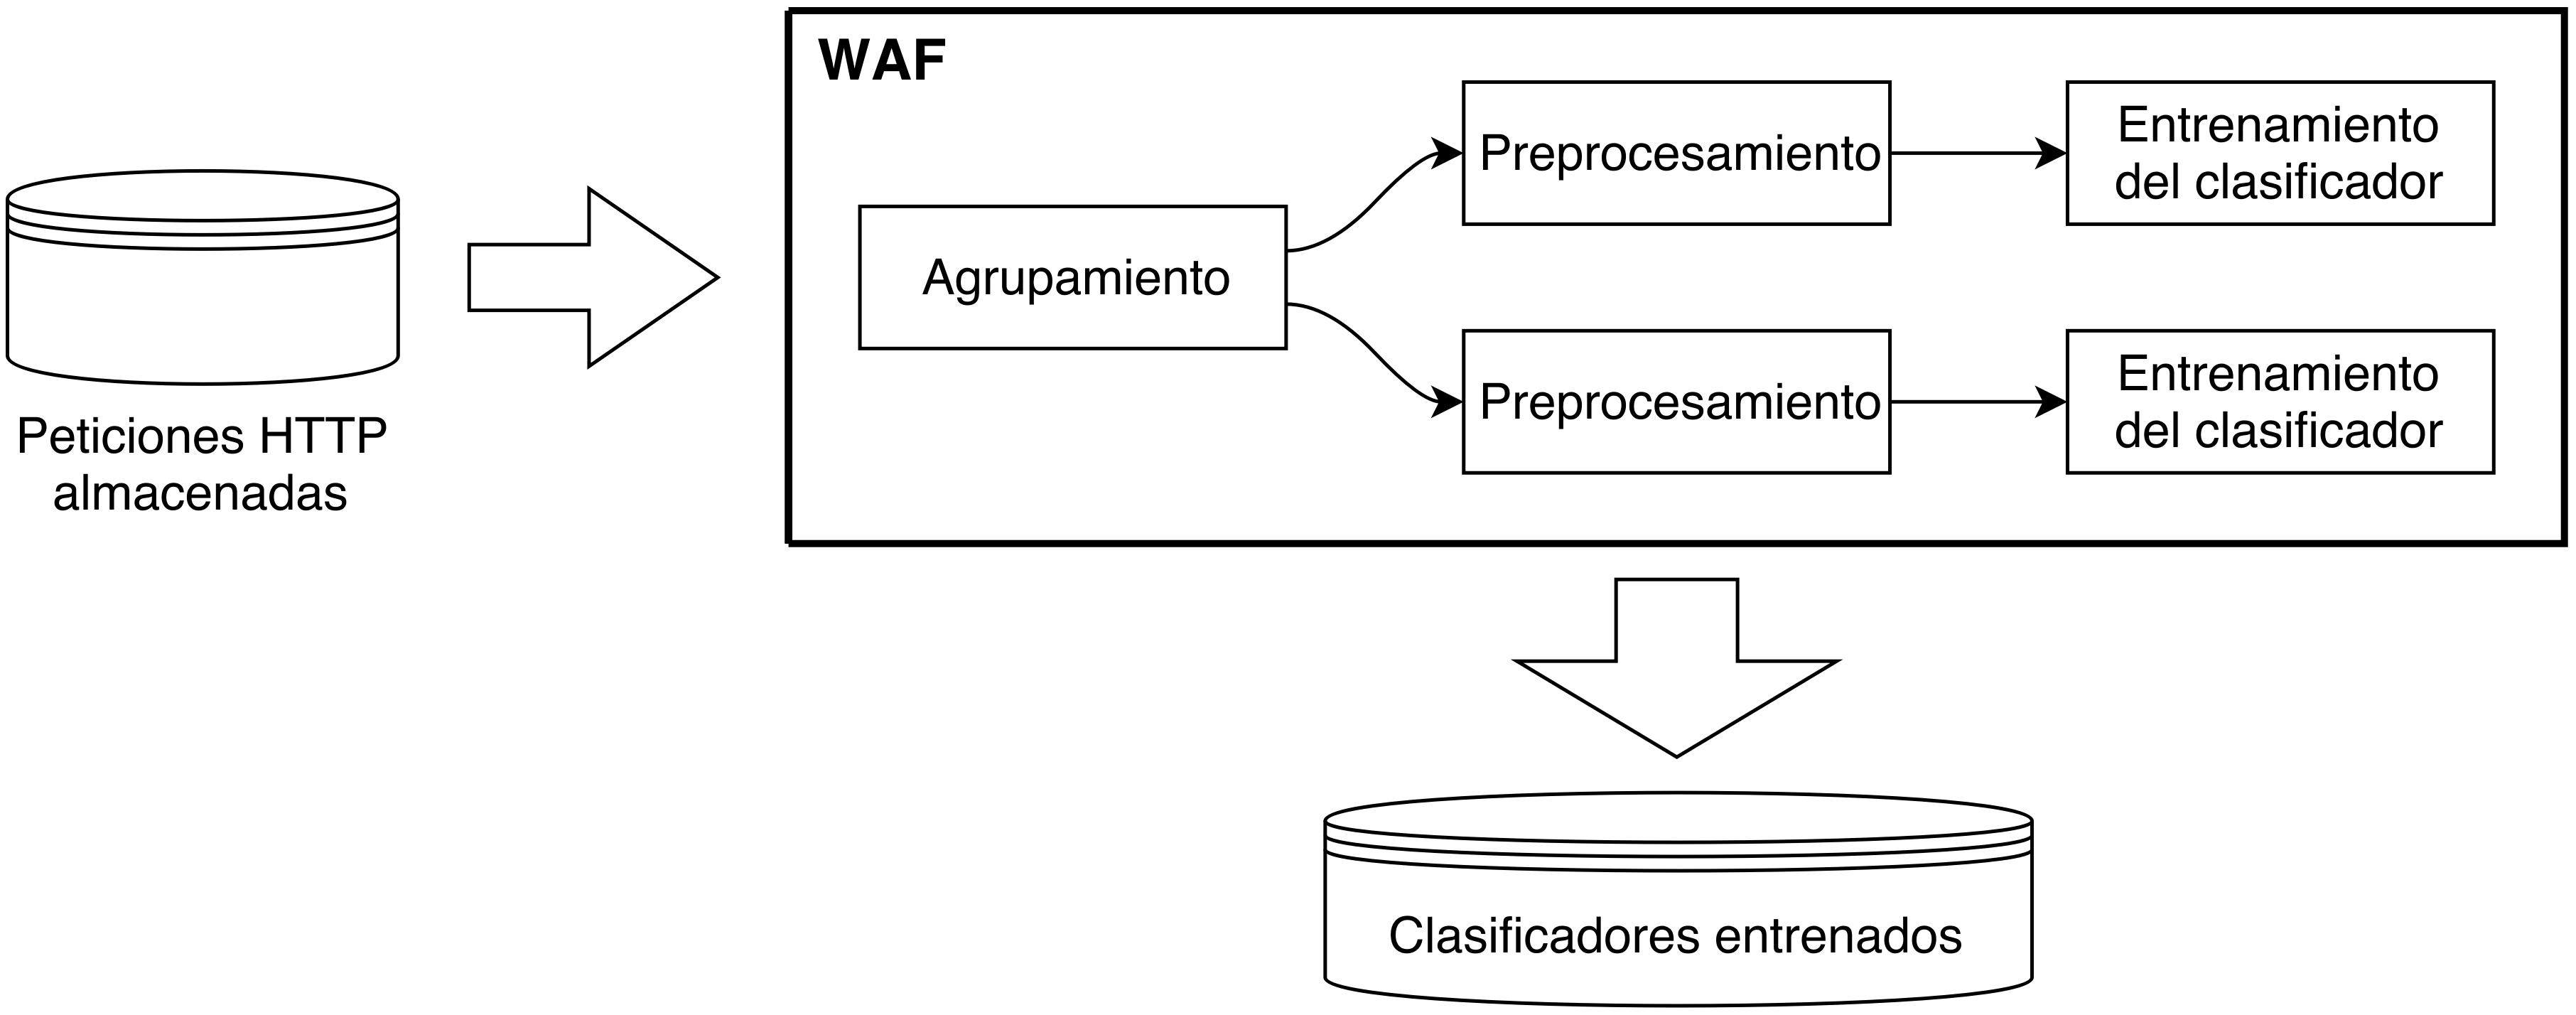
\includegraphics[width=\linewidth]{images/waf-diagram-training.png}

    \caption{Arquitectura de \gls{acr3:name} en la fase de
        entrenamiento.}
    \label{fig:waf:waf_diagram_training}
\end{figure}

Como se puede observar en la figura mencionada, para esta fase se necesitan
peticiones normales (la clase conocida) que representan el tráfico normal
que se espera recibir durante la fase de detección. Se podría usar nuestra
implementación para esta recolección de muestras; para eso se debe proceder
a deshabilitar los procesos de análisis y solamente almacenar las peticiones
que pasen por el detector.


\subsection{Paso de agrupamiento}

Como ya hemos explicado en el \autoref{chap:p3_concepts_features},
agrupamos las peticiones \gls{acr3:http} por método y \gls{acr3:url}
para aprovechar las semejanzas que presentan las peticiones dentro de
un mismo grupo. Partimos de la premisa de que peticiones que van dirigidas
a una misma \gls{acr3:url} y con el mismo método \gls{acr3:http} presentan
más similitudes entre ellas que con peticiones que tienen otro método o
\gls{acr3:url}. Agrupando las peticiones disponibles por método y
\gls{acr3:url} se puede entrenar clasificadores independientes sobre
cada uno de estos grupos. De esta forma se puede obtener modelos de
anomalías más precisos dentro de cada grupo, con el fin de lograr mejores
resultados en la fase de detección.

Utilizando la nomenclatura que hemos introducido en el
\autoref{chap:p3_concepts_features}, podemos denominar \gls{sim3:g} al
conjunto de los grupos de peticiones que se obtienen por este paso de
agrupamiento. Consecuentemente, cada grupo es identificado como \gls{sim3:gi}.


\subsection{Paso de preprocesamiento}

En el paso de preprocesamiento, nuestros procesos de extracción de
\textit{features} son aplicados a las peticiones \gls{acr3:http} para
representarlas con vectores numéricos de \textit{features}.
Este paso se realiza de forma independiente para cada grupo \gls{sim3:gi}.
Debido a eso, en la \autoref{fig:waf:waf_diagram_training} podemos ver
múltiples instancias de preprocesamiento, que corresponden a los distintos
grupos.

Primeramente, como ya hemos explicado en el
\autoref{chap:p3_concepts_features}, \gls{acr3:name} construye las listas
\gls{sim3:qi} y \gls{sim3:bi}, que contienen todos los parámetros que
aparecen en el \textit{query string} y cuerpo de alguna petición dentro
del grupo \gls{sim3:gi}. Las duplicaciones son excluidas, y las listas
son ordenadas de forma alfabética.
Después, nuestra implementación procesa las peticiones de cada grupo
\gls{sim3:gi} para construir los conjuntos de vectores \gls{sim3:fi},
en donde cada petición está representada por un vector de \textit{features}
\gls{sim3:fij}. Así, por cada petición en \gls{sim3:gi}, \gls{acr3:name}
extrae los $m = 10$ \textit{features} de la petición completa, incluyendo
cada una de las seis partes que puede tener dicha petición. Luego se
extraen los valores cuyos parámetros aparezcan en las listas \gls{sim3:qi}
y \gls{sim3:bi}, y se generan $m = 10$ \textit{features} de cada uno de
esos valores.

Los $m = 10$ \textit{features} extraídos analizan distintas características,
que son la distribución de caracteres, la entropía y la cantidad de
caracteres de cada valor. Las funciones utilizadas para la extracción
de estos \textit{features} se encuentran en el directorio
\path{/waf/feature_extraction/} de nuestro repositorio.
Debido a que los \textit{features} ya fueron explicados en detalle en el
\autoref{chap:p3_concepts_features}, a continuación nos limitaremos a una
breve descripción de las tres funciones utilizadas por \gls{acr3:name}
para obtener los \textit{features} para cada valor analizado.

\begin{itemize}
    \item
    \textit{Distribución de caracteres}:
    se calcula la frecuencia relativa de cada carácter, se ordena estas
    frecuencias de forma descendente y se agrupan las mismas en cinco
    intervalos de distintos tamaños.
    Para cada valor analizado, esta función retorna cinco números del
    tipo punto flotante, que corresponden a los cinco intervalos que
    fueron calculados.

    \item
    \textit{Entropía}:
    está función calcula la entropía de un valor según la
    \autoref{eq:fe:entropy}.
    Para cada valor analizado, se retorna un número de tipo punto flotante,
    que corresponde a la entropía calculada.

    \item
    \textit{Cantidad de caracteres}:
    esta función cuenta los caracteres de un valor que pertenecen a
    cuatro categorías definidas, específicamente contando la cantidad
    total de caracteres, la cantidad de dígitos, de letras, y finalmente
    la cantidad de otros caracteres que no sean dígitos ni letras.
    Para cada valor analizado, la función retorna cuatro números de
    tipo punto flotante, que corresponden a las cantidad de las cuatro
    categorías mencionadas.
    Esta función podría retornar números enteros, pero elegimos el tipo
    de dato punto flotante para que se obtenga vectores \gls{sim3:fij}
    homogéneos sin realizar conversiones adicionales posteriormente.
\end{itemize}

Todos los números retornados por estas funciones son concatenados de forma
ordenada para formar el vector \gls{sim3:fij} de cada petición. La dimensión
de estos vectores está definida por la \autoref{eq:fe:number_of_features}.
Cabe resaltar que cada grupo \gls{sim3:gi} puede tener una dimensión
distinta para sus vectores \gls{sim3:fij}, ya que depende de la cantidad
de parámetros de las peticiones del grupo.

Con estos vectores de \textit{features} se construye la matriz \gls{sim3:mi}
de cada grupo, donde los vectores conforman las filas de la matriz.
Luego de obtener la matriz \gls{sim3:mi} del grupo, se procede a escalar
los \textit{features}, que son las columnas de la matriz. Se busca que
cada \textit{feature} tenga promedio cercano a 0 y varianza cercana a 1.

Aclaramos que \gls{acr3:name} puede ser extendido con mucha facilidad
en esta parte de extracción de \textit{features}, agregando o quitando
funciones que analizan los valores.


\subsection{Paso de entrenamiento del clasificador}

Después de realizar la extracción de \textit{features} y el escalamiento
de los mismos, \gls{acr3:name} utiliza las matrices \gls{sim3:mi} obtenidas
para entrenar un clasificador \gls{acr3:ocsvm} para cada grupo \gls{sim3:gi}.
Para el proceso de entrenamiento, el \gls{acr3:ocsvm} recibe la matriz
\gls{sim3:mi} y también los valores para los parámetros \gls{sim3:nui}
y \gls{sim3:gammai} elegidos para ese grupo.
Como ya mencionamos en el \autoref{chap:p3_concepts_ocsvm}, utilizamos
el \textit{kernel} \gls{acr3:rbf} para todos los clasificadores.

Para finalizar esta fase de entrenamiento, \gls{acr3:name} almacena toda
la información necesaria para realizar la detección de anomalías en la
fase de detección. Primeramente se almacenan datos generados por los procesos
de extracción de \textit{features}, que incluye los parámetros extraídos
y su orden dentro de los vectores, luego se persiste los promedios y
desviaciones calculados para el escalamiento de cada \textit{features},
y por último se guarda también el clasificador entrenado.
Nuestra implementación almacenado toda esta información en un archivo
binario en disco, para ser utilizado posteriormente en la fase de detección.

La selección de los valores para los parámetros \gls{sim3:nui} y
\gls{sim3:gammai} presenta un gran desafío. Esto se debe a que durante
la fase de entrenamiento no se cuenta con peticiones anómalas (muestras
positivas) para validar si el clasificador entrenado clasifica correctamente
las anomalías; solamente se puede validarlo contra las peticiones normales.
Esto es un desafío que está presente en los problemas de \gls{acr3:occ},
ya que no se tiene disponible mucho conocimiento sobre las muestras que
no pertenecen a la clase conocida
\citep{khan2009survey}. % from abstract

Una estrategia para encontrar valores adecuados para los dos parámetros
en cuestión puede ser el entrenamiento de un clasificador con solamente
un subconjunto de los datos disponibles, utilizando los datos restantes
para una validación posterior al entrenamiento. Este proceso puede ser
repetido para varios valores distintos de \gls{sim3:nui} y \gls{sim3:gammai},
seleccionando finalmente los valores que resulten en la mejor clasificación
de los datos de entrenamiento.
Utilizamos esta estrategia en las pruebas que realizamos con \gls{acr3:name},
las cuales presentaremos en el siguiente capítulo. Sin embargo, nuestra
implementación no cuenta todavía con un método automático para la selección
de los valores para \gls{sim3:nui} y \gls{sim3:gammai}.


\section{Fase de detección}

En esta fase, \gls{acr3:name} utiliza los procesos de extracción y
los clasificadores entrenados para analizar las peticiones \gls{acr3:http}
entrantes con el fin de determinar si dichas peticiones son normales o
anómalas. Según el resultado de la detección, el \gls{acr3:waf} realiza
distintas acciones configurables para cada caso.

En la \autoref{fig:waf:waf_diagram_detection} se puede observar la
arquitectura de \gls{acr3:name} en esta fase de detección.
Se puede notar cuatro pasos intermedios para esta fase, que son el
enrutamiento de las peticiones a su grupo \gls{sim3:gi} correspondiente,
el preprocesamiento y la clasificación de las mismas, y finalmente las
acciones que son realizadas en respuesta al resultado de la clasificación
de cada petición analizada.

\begin{figure}[ht]
    \centering
    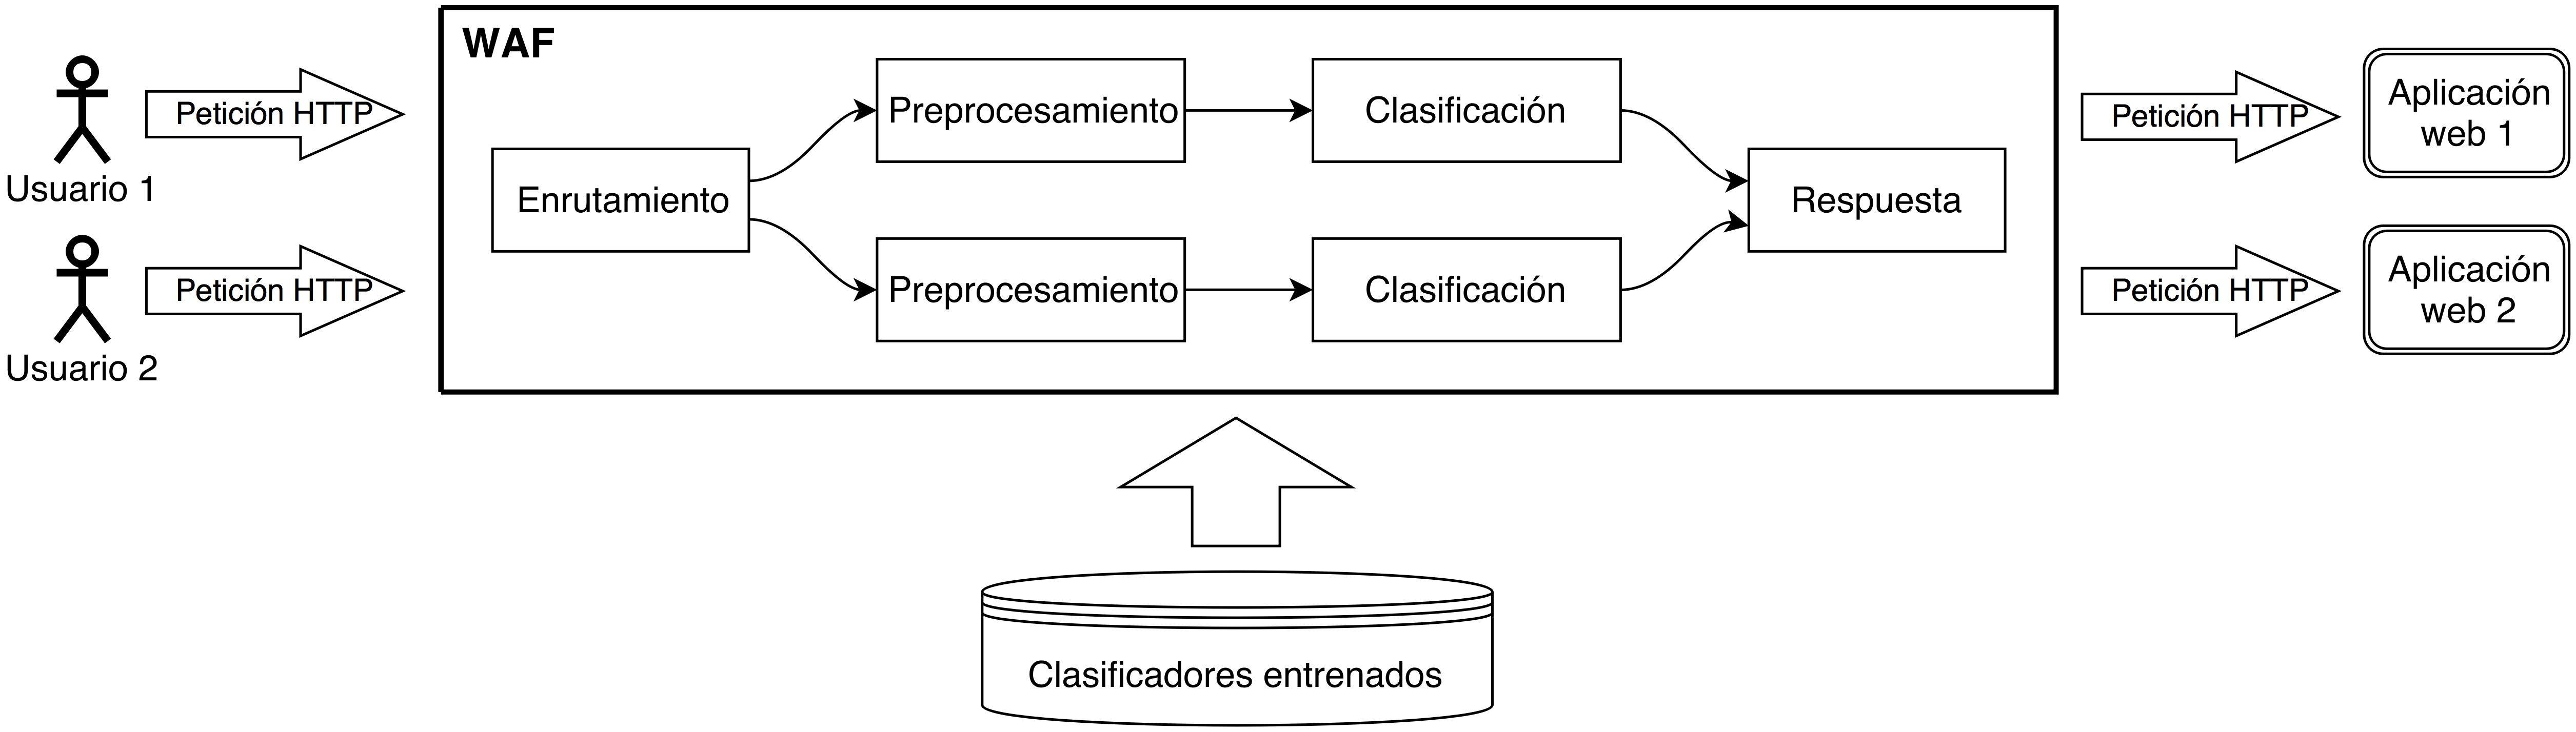
\includegraphics[width=\linewidth]{images/waf-diagram-detection.png}

    \caption{Arquitectura de \gls{acr3:name} en la fase de
        detección.}
    \label{fig:waf:waf_diagram_detection}
\end{figure}


\subsection{Paso de enrutamiento}

Como se puede observar en la \autoref{fig:waf:waf_diagram_detection},
\gls{acr3:name} puede proteger múltiples aplicaciones web y procesar
peticiones de varios usuarios. Los grupos \gls{sim3:gi}, que fueron
formados durante la fase de entrenamiento, pueden ser identificados a
través del método \gls{acr3:http} y la \gls{acr3:url} de sus peticiones.
Para proveer una detección más rápida, \gls{acr3:name} en su proceso de
inicialización ya carga en memoria toda la información almacenada del
entrenamiento, para de esta forma evitar las costosas lecturas de disco
durante el proceso de detección.

De esta forma, este primer paso de enrutamiento determina el grupo
\gls{sim3:gi} correspondiente a cada nueva petición que es recibida
por el \gls{acr3:waf}.
En caso de que no se encuentre el grupo para una petición, \gls{acr3:name}
puede simplemente reenviar dicha petición a su destino por no tener
clasificadores para analizarla, o de lo contrario, puede bloquear dicha
petición por no haber visto peticiones para ese grupo durante el
entrenamiento. Esta configuración queda a cargo de los administradores
responsables por el detector.


\subsection{Paso de preprocesamiento}

Una vez determinado el grupo \gls{sim3:gi} correspondiente a una nueva
petición, \gls{acr3:name} procede a aplicar los procesos de extracción
de \textit{features} a la misma.

Primeramente, se extraen los $m = 10$ \textit{features} de la petición
completa. Luego, utilizando las listas \gls{sim3:qi} y \gls{sim3:bi} del
grupo, los valores de los parámetros de la petición son extraídos y se
generan los $m = 10$ \textit{features} de cada uno.
Atendiendo el orden de los \textit{features}, que fue establecido durante
el entrenamiento, \gls{acr3:name} construye el vector $\vec{x}$ de la
nueva petición. Este nuevo vector tendrá la dimensión correspondiente al
grupo.
Luego se aplica el proceso de escalamiento al vector, usando el promedio
y la desviación estándar calculados para el grupo \gls{sim3:gi}
correspondiente.


\subsection{Paso de clasificación}

En este paso, \gls{acr3:name} emplea el clasificador \gls{acr3:ocsvm}
entrenado del grupo correspondiente para determinar si la nueva petición
será considerada normal o anómala.

El paso de clasificación consiste en aplicar la función de decisión
$g_{i}(\vec{x})$ presentada en la \autoref{eq:ocsvm:decision4} al vector
de \textit{features} $\vec{x}$ que representa a la nueva petición en
cuestión.
Si la clasificación obtiene $g_{i}(\vec{x}) = 1$, entonces la representación
de esta nueva petición en el espacio de dimensiones mayores se encuentra
separada del origen por el hiperplano, indicando que esta petición es
normal (una muestra negativa).
En cambio, si se obtiene $g_{i}(\vec{x}) = -1$, entonces la nueva petición
se encuentra del mismo lado que el origen, indicando que se trata de una
anomalía (una muestra positiva o ataque).


\subsection{Paso de respuesta}

Después de clasificar la nueva petición como normal o anómala, \gls{acr3:name}
procede a realizar las acciones de respuesta que fueron configuradas para
el resultado de clasificación correspondiente.
Si la petición en cuestión es considerada normal, la misma es reenviada
a la aplicación web destino. En cambio, si la petición es considerada
anómala, el resultado de la clasificación y la petición quedan registrados
en un \textit{log}.

Opcionalmente, \gls{acr3:name} puede ser configurado para bloquear las
peticiones anómalas, evitando de esta forma que las mismas lleguen a las
aplicaciones destino. En cambio, si el bloqueo se encuentra deshabilitado,
la petición anómala es reenviada a la aplicación destino, como si fuera
una petición normal.
La configuración del bloqueo de peticiones anómalas queda a cargo de los
administradores responsables, ya que los distintos ambientes de implementación
podrían tener necesidades diferentes. Por ejemplo, ciertos ambientes podrían
preferir bloquear todas las anomalías para evitar posibles ataques. Esto
podría causar que peticiones normales incorrectamente clasificadas no
lleguen a su destino (se producen falsos positivos).
En cambio, otros ambientes podrían optar por solamente lanzar alertas y
no bloquear las anomalías para evitar que peticiones normales erróneamente
clasificadas como anómalas (justamente los falsos positivos mencionados)
no lleguen a su destino y afecten la experiencia de usuarios legítimos.

Además, nuestra implementación puede ser extendida con otras acciones
a realizar en respuesta a la detección de peticiones anómalas. Por ejemplo,
se podría agregar el envío de notificaciones o alarmas en caso de anomalías,
para que los administradores estén enterados al instante y no sea necesario
esperar la inspección de los \textit{logs} para percatarse de distintos
tipos de incidentes de seguridad.


\section{Limitaciones de la implementación}

Nuestra implementación busca ser funcional y sencilla. Se trata de una
prueba de concepto, y por este motivo no nos hemos enfocado en obtener
una aplicación terminada que incluya todas las funcionalidades necesarias
para ser utilizada directamente en ambientes de producción.
A continuación, mencionamos las limitaciones que están presentes en el
\gls{acr3:waf} que implementamos en el marco de este trabajo:

\begin{itemize}
    \item
    \gls{acr3:name} no cuenta con un panel de administración para visualizar
    el estado del mismo o realizar cambios en las configuraciones. Se debe
    realizar el inicio del detector mediante un \textit{script}, utilizando
    parámetros para seleccionar las opciones de configuración.

    \item
    \gls{acr3:name} podría ser utilizado para la recolección de peticiones
    normales para la fase de entrenamiento. Los procesos de detección
    pueden ser deshabilitados indicando la configuración deseada al momento
    de inicialización del \gls{acr3:waf}, pero nuestra implementación
    no cuenta todavía con mecanismos para almacenar las peticiones en
    memoria secundaria.

    \item
    Para el entrenamiento de los clasificadores, \gls{acr3:name} no
    cuenta todavía con un método automático para la selección de los
    valores para los parámetros \gls{sim3:nui} y \gls{sim3:gammai},
    de forma que estos deben ser especificados por los administradores
    del detector.
\end{itemize}

En el siguiente capítulo presentamos las pruebas que realizamos con nuestra
implementación y los resultados que obtuvimos mediante las mismas.

    \renewcommand{\newCommandChapterTitle}{Pruebas y resultados}
\chapter{\newCommandChapterTitle}
\markright{\hfill \thechapter. \newCommandChapterTitle}
\label{chap:p3_results}


En este capítulo presentamos las pruebas que realizamos con \gls{acr3:name}.
Primeramente describimos los conjuntos de datos de prueba utilizados,
luego explicamos las pruebas realizadas y finalmente comparamos los
resultados obtenidos con otros trabajos relacionados.


\section{Conjuntos de datos de prueba}

Para evaluaciones cuantitativas de la eficacia de detección del
\gls{acr3:waf} que hemos implementado necesitamos conjuntos de datos.
Obtener buenos datos para las pruebas es fundamental para obtener
resultados que después se comprueben en el mundo real.
Pero esto no es una tarea fácil, ya que muchos conjuntos de datos tienen
ciertas falencias que los hacen poco útiles para nuestras pruebas
\citep{torranoGimenez2015study}.

\subsection{Características deseadas para los conjuntos de datos}

Según \citep{torranoGimenez2015study} los conjuntos de
datos utilizados en las investigaciones sobre \gls{acr3:waf} deberían
cumplir ciertos criterios para ser de utilidad para la comunidad
científica. Algunas de esas características son:

\begin{itemize}
    \item
    Deberían ser públicos para que investigadores puedan comparar
    resultados.

    \item
    Deberían contener tráfico \gls{acr3:http}, ya que se trata de un
    \gls{acr3:waf}.

    \item
    Deberían contener datos etiquetados según sean normales o anómalas.

    \item
    Deberían incluir ataques novedosos y relevantes.
\end{itemize}

Los trabajos relacionados sobre \gls{acr3:waf} utilizan distintos conjuntos
de datos para sus pruebas, pero la mayoría de esos conjuntos no cumple una
o varias de las características mencionadas anteriormente
\citep{torranoGimenez2015study}.
Encontramos dos conjuntos de datos adecuados según los criterios mencionados;
fueron creados por el Consejo Superior de Investigaciones Científicas
(\gls{acr3:csic}) de España y publicados como \gls{acr3:csic} 2010
\citep{csic2010dataset} y \gls{acr3:csic} TORPEDA 2012 \citep{torpeda2012dataset}.
Varias investigaciones relacionadas ya utilizaron estos conjuntos, como
por ejemplo \citep{parhizkar2015oc} y \citep{torranoGimenez2015study},
y así podemos comparar resultados con dichos trabajos.


\subsection{Descripción de los conjuntos de datos utilizados}

Los dos conjuntos de datos del \gls{acr3:csic} contienen peticiones
\gls{acr3:http} hechas a una aplicación sencilla de comercio electrónico,
simulando distintos escenarios como, por ejemplo, registro de clientes
y compra de productos. Una descripción más detallada sobre el proceso
de creación de estos conjuntos se puede encontrar en el trabajo
\citep{torranoGimenez2015study}.

El conjunto \gls{acr3:csic} 2010 \citep{csic2010dataset} consiste de tres
archivos: dos archivos de 20 \gls{acr3:mb} con tráfico \gls{acr3:http}
normal, que contienen alrededor de \num{72000} peticiones, y un archivo
de 15 \gls{acr3:mb} con tráfico anómalo, que contiene cerca de \num{25000}
peticiones. Este último archivo contiene varios tipos de ataques, además
de anomalías que no necesariamente son ataques pero representan peticiones
con datos no esperados.

Considerando que nuestro \gls{acr3:waf} entrena un clasificador por cada
combinación de \gls{acr3:url} y método \gls{acr3:http}, nosotros agrupamos
todas las peticiones de los tres archivos por este criterio.
De esta manera obtuvimos más de \num{1600} grupos distintos, pero notamos
que muchos de ellos tenían solamente peticiones normales o solamente
peticiones anómalas. Esos casos no nos sirven para las pruebas, ya que
necesitamos datos normales para el entrenamiento y posteriormente anomalías
para validar que el \gls{acr3:waf} detecta correctamente estas últimas.
Por este motivo decidimos utilizar solamente aquellos grupos que tienen
más de 100 peticiones normales y también más de 100 peticiones anómalas.
Así obtuvimos 16 grupos, alcanzando un total de \num{32000} peticiones
normales y \num{19160} anómalas.
En la \autoref{tbl:res:selected_data_sets} se pueden ver en detalle los grupos
de peticiones que utilizamos para nuestras pruebas, incluyendo un identificador
corto que le asignamos a cada uno de los grupos para la mejor visualización
de los resultados.

El conjunto de datos \gls{acr3:csic} TORPEDA 2012 \citep{torpeda2012dataset}
consiste de ocho archivos: un archivo de 8 \gls{acr3:mb} con tráfico
\gls{acr3:http} normal, que contiene alrededor de \num{8000} peticiones,
y siete archivos totalizando más de 60 \gls{acr3:mb} de tráfico anómalo,
que contienen más de \num{65000} peticiones con ataques y también anomalías
no maliciosas.

\begin{table}[ht]
    \centering
    \small
    \begin{tabularx}{\linewidth}{|C|c|ll|r|r|r|}
        \hline
        ID
        & \multicolumn{1}{c|}{\begin{tabular}[c]{@{}c@{}}Conjunto\\ de datos\\ CSIC\end{tabular}}
        & \multicolumn{2}{c|}{Método HTTP y URL}
        & \multicolumn{1}{c|}{\begin{tabular}[c]{@{}c@{}}Cant.\\ parám.\end{tabular}}
        & \multicolumn{1}{c|}{\begin{tabular}[c]{@{}c@{}}Peticiones\\ normales\end{tabular}}
        & \multicolumn{1}{c|}{\begin{tabular}[c]{@{}c@{}}Peticiones\\ anómalas\end{tabular}} \\
        \specialrule{1.5pt}{0}{0}
        c00 & 2010  & GET  & /tienda1/miembros/editar.jsp         & 13 &  \num{2000} &  \num{1362} \\ \hline
        c01 & 2010  & POST & /tienda1/miembros/editar.jsp         & 13 &  \num{2000} &  \num{1362} \\ \hline
        c02 & 2010  & GET  & /tienda1/publico/anadir.jsp          &  5 &  \num{2000} &  \num{1380} \\ \hline
        c03 & 2010  & POST & /tienda1/publico/anadir.jsp          &  5 &  \num{2000} &  \num{1380} \\ \hline
        c04 & 2010  & GET  & /tienda1/publico/autenticar.jsp      &  5 &  \num{2000} &  \num{1361} \\ \hline
        c05 & 2010  & POST & /tienda1/publico/autenticar.jsp      &  5 &  \num{2000} &  \num{1361} \\ \hline
        c06 & 2010  & GET  & /tienda1/publico/caracteristicas.jsp &  1 &  \num{2000} &   \num{954} \\ \hline
        c07 & 2010  & POST & /tienda1/publico/caracteristicas.jsp &  1 &  \num{2000} &   \num{954} \\ \hline
        c08 & 2010  & GET  & /tienda1/publico/entrar.jsp          &  1 &  \num{2000} &   \num{897} \\ \hline
        c09 & 2010  & POST & /tienda1/publico/entrar.jsp          &  1 &  \num{2000} &   \num{897} \\ \hline
        c10 & 2010  & GET  & /tienda1/publico/pagar.jsp           &  3 &  \num{2000} &  \num{1343} \\ \hline
        c11 & 2010  & POST & /tienda1/publico/pagar.jsp           &  3 &  \num{2000} &  \num{1343} \\ \hline
        c12 & 2010  & GET  & /tienda1/publico/registro.jsp        & 13 &  \num{2000} &  \num{1364} \\ \hline
        c13 & 2010  & POST & /tienda1/publico/registro.jsp        & 13 &  \num{2000} &  \num{1364} \\ \hline
        c14 & 2010  & GET  & /tienda1/publico/vaciar.jsp          &  1 &  \num{2000} &   \num{919} \\ \hline
        c15 & 2010  & POST & /tienda1/publico/vaciar.jsp          &  1 &  \num{2000} &   \num{919} \\ \hline
        t00 & 2012  & POST & /tienda1/miembros/editar.jsp         & 12 &  \num{5608} & \num{10121} \\ \hline
        t01 & 2012  & POST & /tienda1/publico/registro.jsp        & 12 &  \num{2522} & \num{13163} \\
        \specialrule{1.5pt}{0}{0}
            & Total &      &                                      &    & \num{40130} & \num{42444} \\ \hline
    \end{tabularx}

    \caption{Peticiones seleccionadas de los conjuntos de datos para nuestras
        pruebas, agrupadas por método \gls{acr3:http} y \gls{acr3:url}.}
    \label{tbl:res:selected_data_sets}
\end{table}

Realizando de vuelta la agrupación de las peticiones obtuvimos 72 grupos
distintos, pero también había casos con solamente peticiones normales
o solamente anomalías. Después de seleccionar únicamente aquellos con
más de 100 peticiones normales y también más de 100 peticiones anómalas,
nos quedamos con 2 grupos, alcanzando un total de \num{8130} peticiones
normales y \num{23284} anómalas.
En la ya mencionada \autoref{tbl:res:selected_data_sets} se pueden ver los
detalles de estos grupos también.


\section{Análisis de la eficacia de detección}

Realizamos pruebas para analizar la eficacia de detección de \gls{acr3:name},
utilizando los conjuntos de datos presentados. Con el fin de agilizar el
proceso de extracción de \textit{features} y realizar la clasificación
de forma más eficiente, para estas pruebas construimos una versión
reducida del \gls{acr3:waf} que no incluye recepción y envío de peticiones,
sino que obtiene las peticiones de un archivo. El código se encuentra en
el directorio \path{/tests/detection_efficacy/}.

Cabe volver a mencionar que nuestra implementación no contiene todavía
un mecanismo automático para la selección de los valores para los parámetros
\gls{sim3:nui} y \gls{sim3:gammai} de los clasificadores. Para estas
pruebas, realizamos una búsqueda en el rango $[\num{0.0001} ; \num{0.1}]$
para ambos parámetros y seleccionamos los valores que obtuvieron los
mejores resultados en la fase de detección para cada grupo de peticiones.
Cada búsqueda fue realizada tres veces, utilizando cada vez un subconjunto
distinto de peticiones para el entrenamiento, con el fin de evitar resultados
dependientes de la selección particular de muestras.
Con esto metodología utilizada mostramos que existen valores para los
parámetros \gls{sim3:nui} y \gls{sim3:gammai} de los clasificadores con
los cuales se puede obtener los resultados de detección que son presentados
a continuación.

\begin{figure}[th]
    \centering
    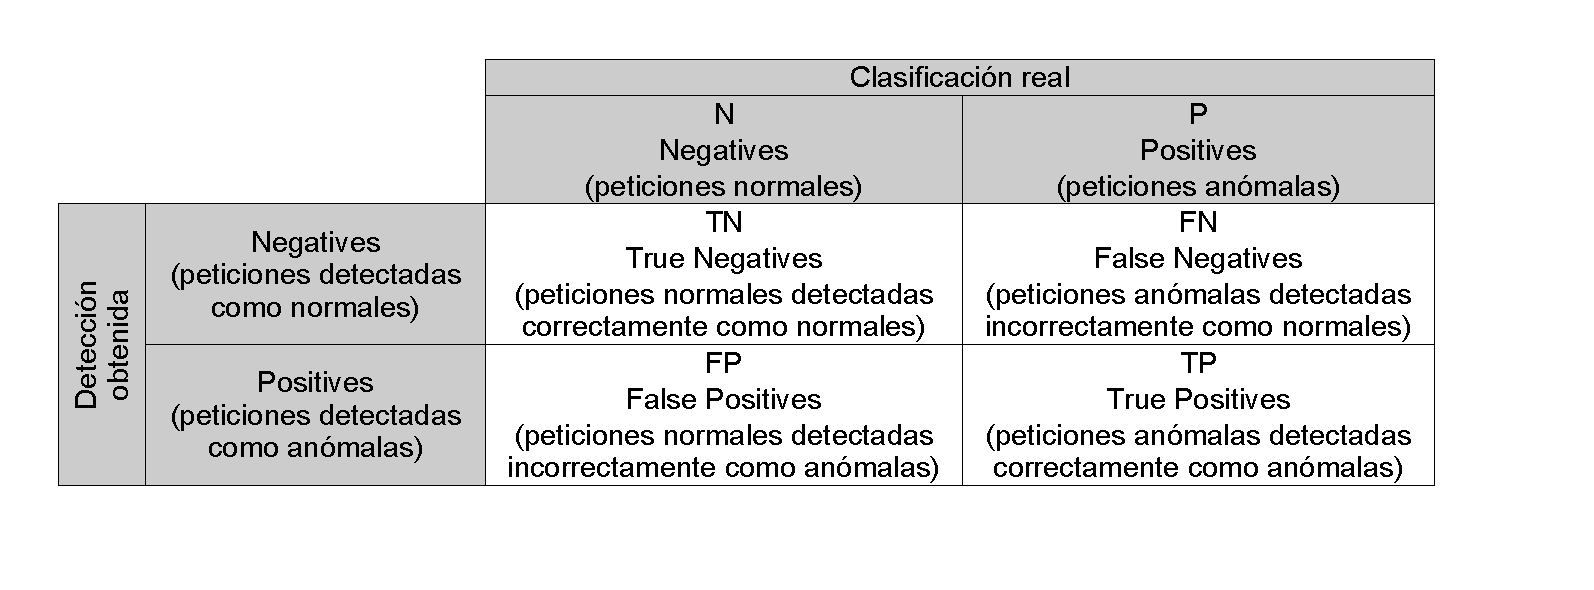
\includegraphics[width=\linewidth, trim=1.1cm 1.7cm 1.6cm 1cm]{images/diagram-score-explanation.pdf}

    \caption{Matriz de confusión de los posibles resultados de clasificación.}
    \label{fig:res:score_explanation}
\end{figure}

Para la cuantificación de las pruebas, tomamos en cuenta los distintos
resultados de clasificación que se puede obtener en la terminología de
\gls{acr3:ids}, según la matriz de confusión ilustrada en la
\autoref{fig:res:score_explanation}.
Se puede observar que la cantidad total de peticiones en la fase de
detección se compone de las peticiones normales (N, o muestras negativas)
y las anomalías o ataques (P, o muestras positivas).

Las peticiones normales pueden ser detectadas como tales, resultando en
negativos correctos (TN), o pueden ser detectadas como peticiones no
pertenecientes a la clase conocida de los normales, resultando en falsos
positivos (FP).
De la misma forma, las peticiones anómalas pueden ser detectadas como
tales, resultando en positivos correctos (TP), o pueden ser detectadas
erróneamente como pertenecientes a los mensajes normales, resultando en
falsos negativos (FN).
Estas cantidades y las relaciones entre ellas también pueden ser expresadas
como se puede observar en la \autoref{eq:res:scores1}.

\begin{equation}
    \label{eq:res:scores1}
    \text{Total de muestras} = \text{N} + \text{P}
    \ , \quad
    \text{N} = \text{TN} + \text{FP}
    \ , \quad
    \text{P} = \text{TP} + \text{FN}
\end{equation}

Para el análisis de nuestros resultados utilizamos varias métricas que
son fórmulas agregadas de estas cantidades vistas.

\begin{itemize}
    \item
    \textit{True Positives Rate} (\gls{acr3:tpr}):
    Esta métrica indica la fracción de peticiones anómalas (muestras
    positivas) que fue detectada correctamente; tiene un rango $[0;1]$.
    El valor debería ser cercano a 1 para que el \gls{acr3:waf} detecte
    la mayor cantidad posible de ataques antes de que lleguen a las
    aplicaciones protegidas.

    \item
    \textit{False Positives Rate} (\gls{acr3:fpr}):
    Esta métrica indica la fracción de peticiones normales (muestras
    negativas) que fue detectada equivocadamente como anomalías; tiene
    un rango $[0;1]$.
    El valor debería ser cercano a 0 para que el \gls{acr3:waf} no afecte
    negativamente la experiencia de usuarios legítimos de las aplicaciones
    protegidas al bloquear peticiones normales.

    \item
    F$_{1}$-\textit{score}:
    Esta métrica busca incorporar las dos métricas anteriores en un solo
    indicador; tiene también un rango $[0;1]$.
    El valor debería ser también cercano a 1 en los resultados producidos
    por el \gls{acr3:waf} para cumplir los dos objetivos mencionados
    acerca del \gls{acr3:tpr} (detectar todos los ataques) y \gls{acr3:fpr}
    (no afectar usuarios legítimos).
\end{itemize}

Estas tres métricas pueden ser expresadas también con las expresiones
que podemos observar en la \autoref{eq:res:scores2}.

\begin{equation}
    \label{eq:res:scores2}
    \text{TPR} = \frac{\text{TP}}{\text{P}}
    \ , \quad
    \text{FPR} = \frac{\text{FP}}{\text{N}}
    \ , \quad
    \text{F}_{1} = \frac{2 \text{TP}}{2 \text{TP} + \text{FP} + \text{FN}}
\end{equation}

En el análisis de la eficacia de detección de \gls{acr3:name} nos enfocamos
en cuatro aspectos; las mejoras obtenidas por incluir el escalamiento de
los \textit{features}, las mejoras que produce el análisis de los valores
de los parámetros en las peticiones, la influencia de la cantidad de
peticiones utilizadas para el entrenamiento y finalmente la influencia
de peticiones anómalas presentes en los datos de entrenamiento.


\subsection{Mejoras obtenidas por el escalamiento de \textit{features}}

Como ya explicamos en el \autoref{chap:p3_concepts_features}, después
de la extracción de \textit{features} realizamos un escalamiento para
obtener promedio cercano a 0 y varianza cercana a 1 para cada \textit{feature}
de los datos de entrenamiento. Según la teoría, este preprocesamiento ayuda
a mejorar la capacidad de clasificación del \gls{acr3:ocsvm}
\citep{rieck2009machine}, % from section 2.3.1 - normalization of numerical features
y con los resultados de esta prueba logramos comprobar esto.

\begin{table}[ht]
    \centering
    \small
    \begin{tabularx}{\linewidth}{|c|CCC|CCC|}
        \hline
        ID  & \multicolumn{3}{c|}{Sin escalamiento}                                                   & \multicolumn{3}{c|}{Con escalamiento}                                                   \\
            & \gls{acr3:tpr}              & \gls{acr3:fpr}              & F$_{1}$-\textit{score}      & \gls{acr3:tpr}              & \gls{acr3:fpr}              & F$_{1}$-\textit{score}      \\
        \specialrule{1.5pt}{0}{0}
        c00 & \num{0.85} $\pm$ \num{0.01} & \num{0.31} $\pm$ \num{0.01} & \num{0.73} $\pm$ \num{0.00} & \num{0.71} $\pm$ \num{0.01} & \num{0.05} $\pm$ \num{0.00} & \num{0.80} $\pm$ \num{0.00} \\ \hline
        c01 & \num{0.85} $\pm$ \num{0.00} & \num{0.32} $\pm$ \num{0.00} & \num{0.73} $\pm$ \num{0.00} & \num{0.72} $\pm$ \num{0.01} & \num{0.05} $\pm$ \num{0.01} & \num{0.80} $\pm$ \num{0.00} \\ \hline
        c02 & \num{0.93} $\pm$ \num{0.12} & \num{0.13} $\pm$ \num{0.10} & \num{0.88} $\pm$ \num{0.01} & \num{1.00} $\pm$ \num{0.00} & \num{0.03} $\pm$ \num{0.01} & \num{0.98} $\pm$ \num{0.01} \\ \hline
        c03 & \num{0.87} $\pm$ \num{0.12} & \num{0.08} $\pm$ \num{0.12} & \num{0.88} $\pm$ \num{0.01} & \num{1.00} $\pm$ \num{0.00} & \num{0.03} $\pm$ \num{0.00} & \num{0.98} $\pm$ \num{0.00} \\ \hline
        c04 & \num{0.97} $\pm$ \num{0.01} & \num{0.25} $\pm$ \num{0.01} & \num{0.83} $\pm$ \num{0.01} & \num{0.91} $\pm$ \num{0.01} & \num{0.01} $\pm$ \num{0.00} & \num{0.95} $\pm$ \num{0.01} \\ \hline
        c05 & \num{0.96} $\pm$ \num{0.01} & \num{0.26} $\pm$ \num{0.01} & \num{0.82} $\pm$ \num{0.01} & \num{0.92} $\pm$ \num{0.01} & \num{0.01} $\pm$ \num{0.00} & \num{0.95} $\pm$ \num{0.00} \\ \hline
        c06 & \num{0.99} $\pm$ \num{0.00} & \num{0.08} $\pm$ \num{0.06} & \num{0.92} $\pm$ \num{0.05} & \num{0.99} $\pm$ \num{0.00} & \num{0.00} $\pm$ \num{0.00} & \num{1.00} $\pm$ \num{0.00} \\ \hline
        c07 & \num{0.99} $\pm$ \num{0.01} & \num{0.11} $\pm$ \num{0.01} & \num{0.88} $\pm$ \num{0.01} & \num{0.99} $\pm$ \num{0.00} & \num{0.00} $\pm$ \num{0.00} & \num{1.00} $\pm$ \num{0.00} \\ \hline
        c08 & \num{0.99} $\pm$ \num{0.02} & \num{0.01} $\pm$ \num{0.00} & \num{0.98} $\pm$ \num{0.01} & \num{1.00} $\pm$ \num{0.00} & \num{0.00} $\pm$ \num{0.00} & \num{1.00} $\pm$ \num{0.00} \\ \hline
        c09 & \num{0.98} $\pm$ \num{0.03} & \num{0.01} $\pm$ \num{0.01} & \num{0.99} $\pm$ \num{0.02} & \num{1.00} $\pm$ \num{0.00} & \num{0.00} $\pm$ \num{0.00} & \num{1.00} $\pm$ \num{0.00} \\ \hline
        c10 & \num{1.00} $\pm$ \num{0.00} & \num{0.14} $\pm$ \num{0.03} & \num{0.90} $\pm$ \num{0.02} & \num{1.00} $\pm$ \num{0.00} & \num{0.00} $\pm$ \num{0.00} & \num{1.00} $\pm$ \num{0.00} \\ \hline
        c11 & \num{1.00} $\pm$ \num{0.00} & \num{0.16} $\pm$ \num{0.02} & \num{0.90} $\pm$ \num{0.01} & \num{1.00} $\pm$ \num{0.00} & \num{0.01} $\pm$ \num{0.00} & \num{0.99} $\pm$ \num{0.00} \\ \hline
        c12 & \num{0.86} $\pm$ \num{0.01} & \num{0.31} $\pm$ \num{0.02} & \num{0.75} $\pm$ \num{0.01} & \num{0.74} $\pm$ \num{0.00} & \num{0.05} $\pm$ \num{0.01} & \num{0.81} $\pm$ \num{0.01} \\ \hline
        c13 & \num{0.86} $\pm$ \num{0.01} & \num{0.32} $\pm$ \num{0.01} & \num{0.74} $\pm$ \num{0.00} & \num{0.74} $\pm$ \num{0.00} & \num{0.05} $\pm$ \num{0.01} & \num{0.81} $\pm$ \num{0.01} \\ \hline
        c14 & \num{0.96} $\pm$ \num{0.04} & \num{0.01} $\pm$ \num{0.01} & \num{0.97} $\pm$ \num{0.02} & \num{1.00} $\pm$ \num{0.00} & \num{0.00} $\pm$ \num{0.00} & \num{1.00} $\pm$ \num{0.00} \\ \hline
        c15 & \num{0.94} $\pm$ \num{0.01} & \num{0.01} $\pm$ \num{0.01} & \num{0.96} $\pm$ \num{0.00} & \num{1.00} $\pm$ \num{0.00} & \num{0.00} $\pm$ \num{0.00} & \num{1.00} $\pm$ \num{0.00} \\ \hline
        t00 & \num{1.00} $\pm$ \num{0.00} & \num{0.07} $\pm$ \num{0.04} & \num{0.98} $\pm$ \num{0.01} & \num{0.99} $\pm$ \num{0.01} & \num{0.06} $\pm$ \num{0.04} & \num{0.98} $\pm$ \num{0.00} \\ \hline
        t01 & \num{0.99} $\pm$ \num{0.01} & \num{0.09} $\pm$ \num{0.10} & \num{0.99} $\pm$ \num{0.01} & \num{1.00} $\pm$ \num{0.00} & \num{0.09} $\pm$ \num{0.06} & \num{0.99} $\pm$ \num{0.01} \\
        \specialrule{1.5pt}{0}{0}
            & \num{0.94} $\pm$ \num{0.07} & \num{0.15} $\pm$ \num{0.12} & \num{0.88} $\pm$ \num{0.09} & \num{0.93} $\pm$ \num{0.11} & \num{0.03} $\pm$ \num{0.03} & \num{0.95} $\pm$ \num{0.08} \\ \hline
    \end{tabularx}

    \caption{Resultados de detección que muestran las mejoras obtenidas
        por el escalamiento de \textit{features}, incluyendo el análisis
        de valores de parámetros.}
    \label{tbl:res:results_scaling}
\end{table}

En la \autoref{tbl:res:results_scaling} se puede observar los resultados
de la clasificación sin y con escalamiento. Para ambos casos usamos 1500
peticiones para el entrenamiento de cada grupo (cerca del 75\% de las
muestras) e incluimos los \textit{features} del análisis de valores de
parámetros.
Al observar los resultados promedios de los grupos de peticiones (la
última fila de la tabla), se puede ver que con el escalamiento el
F$_{1}$-\textit{score} aumenta de \num{0.88} y \num{0.95}, ya que a
pesar de que el \gls{acr3:tpr} promedio baja de \num{0.94} a \num{0.93},
el \gls{acr3:fpr} mejora considerablemente de \num{0.15} a \num{0.03}.

Estos resultados pueden ser observados también en forma gráfica en la
\autoref{fig:res:results_scaling}, donde se compara el F$_{1}$-\textit{score}
obtenido en el proceso de detección sin y con escalamiento para cada
uno de los 18 grupos de peticiones.

\begin{figure}[ht]
    \centering
    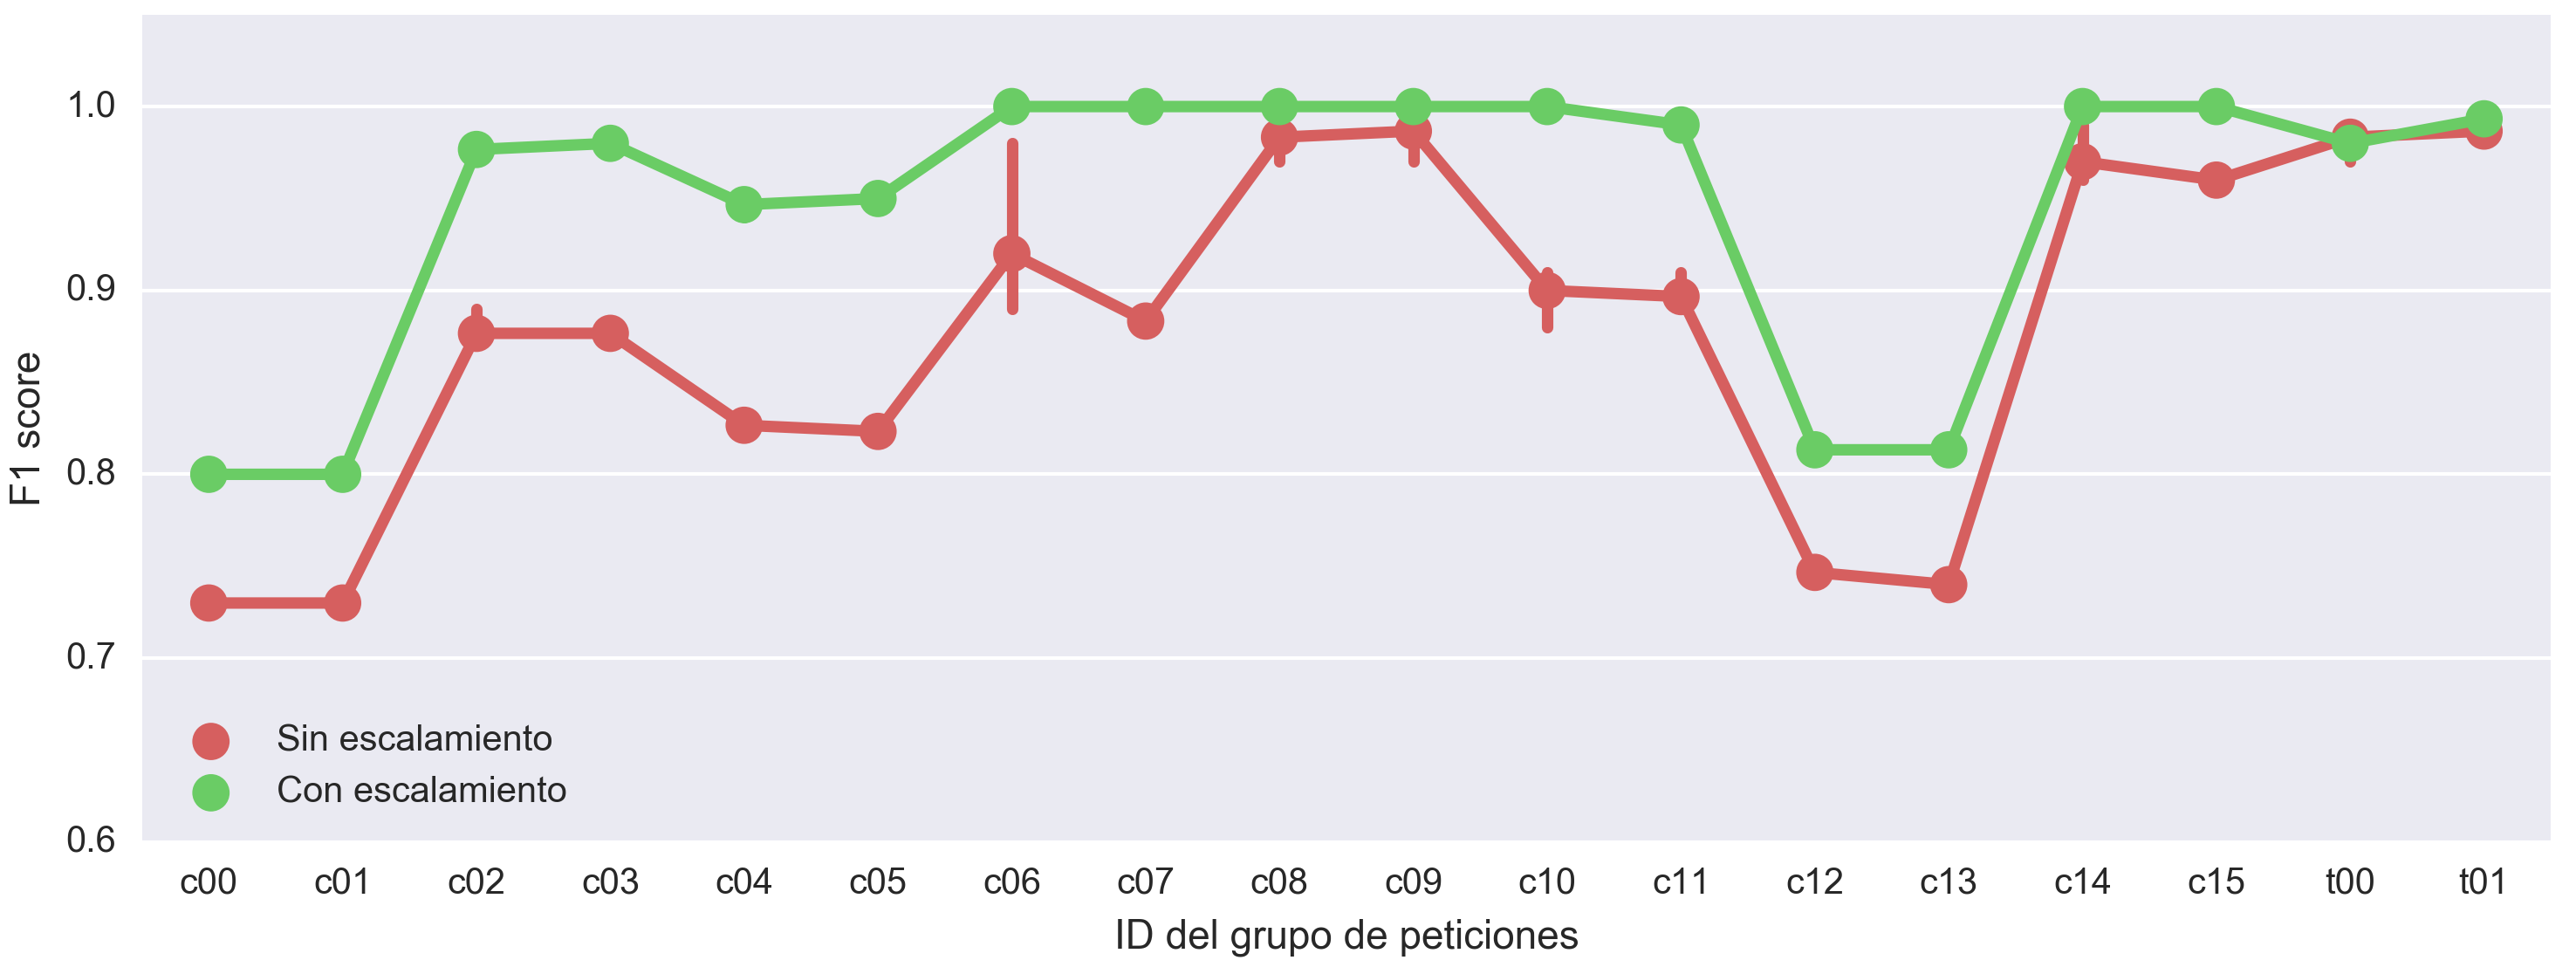
\includegraphics[width=\linewidth]{images/results-scaling.png}

    \caption{Resultados de detección que muestran las mejoras obtenidas
        por el escalamiento de \textit{features}, incluyendo el análisis
        de valores de parámetros.}
    \label{fig:res:results_scaling}
\end{figure}

De esta forma, los resultados nos confirman que el escalamiento de los
\textit{features} mejora la capacidad de clasificación de nuestro
\gls{acr3:ocsvm} para la detección de anomalías en peticiones \gls{acr3:http},
al menos para el conjunto de datos que utilizamos.


\subsection{Mejoras obtenidas por el análisis de valores de parámetros}

Nuestros procesos de extracción de \textit{features} en primer lugar
analizan la petición completa, que resulta en una cantidad fija de
\textit{features} que se obtiene para cada petición.
Adicionalmente, estos procesos analizan también los valores de los
parámetros del \textit{query string} y del cuerpo de las peticiones,
lo que resulta en \textit{features} adicionales cuya cantidad depende
de la cantidad de parámetros de las peticiones de cada grupo. En esta
prueba mostramos que estos \textit{features} adicionales pueden mejorar
la detección de \gls{acr3:name}.

\begin{figure}[hbt]
    \centering
    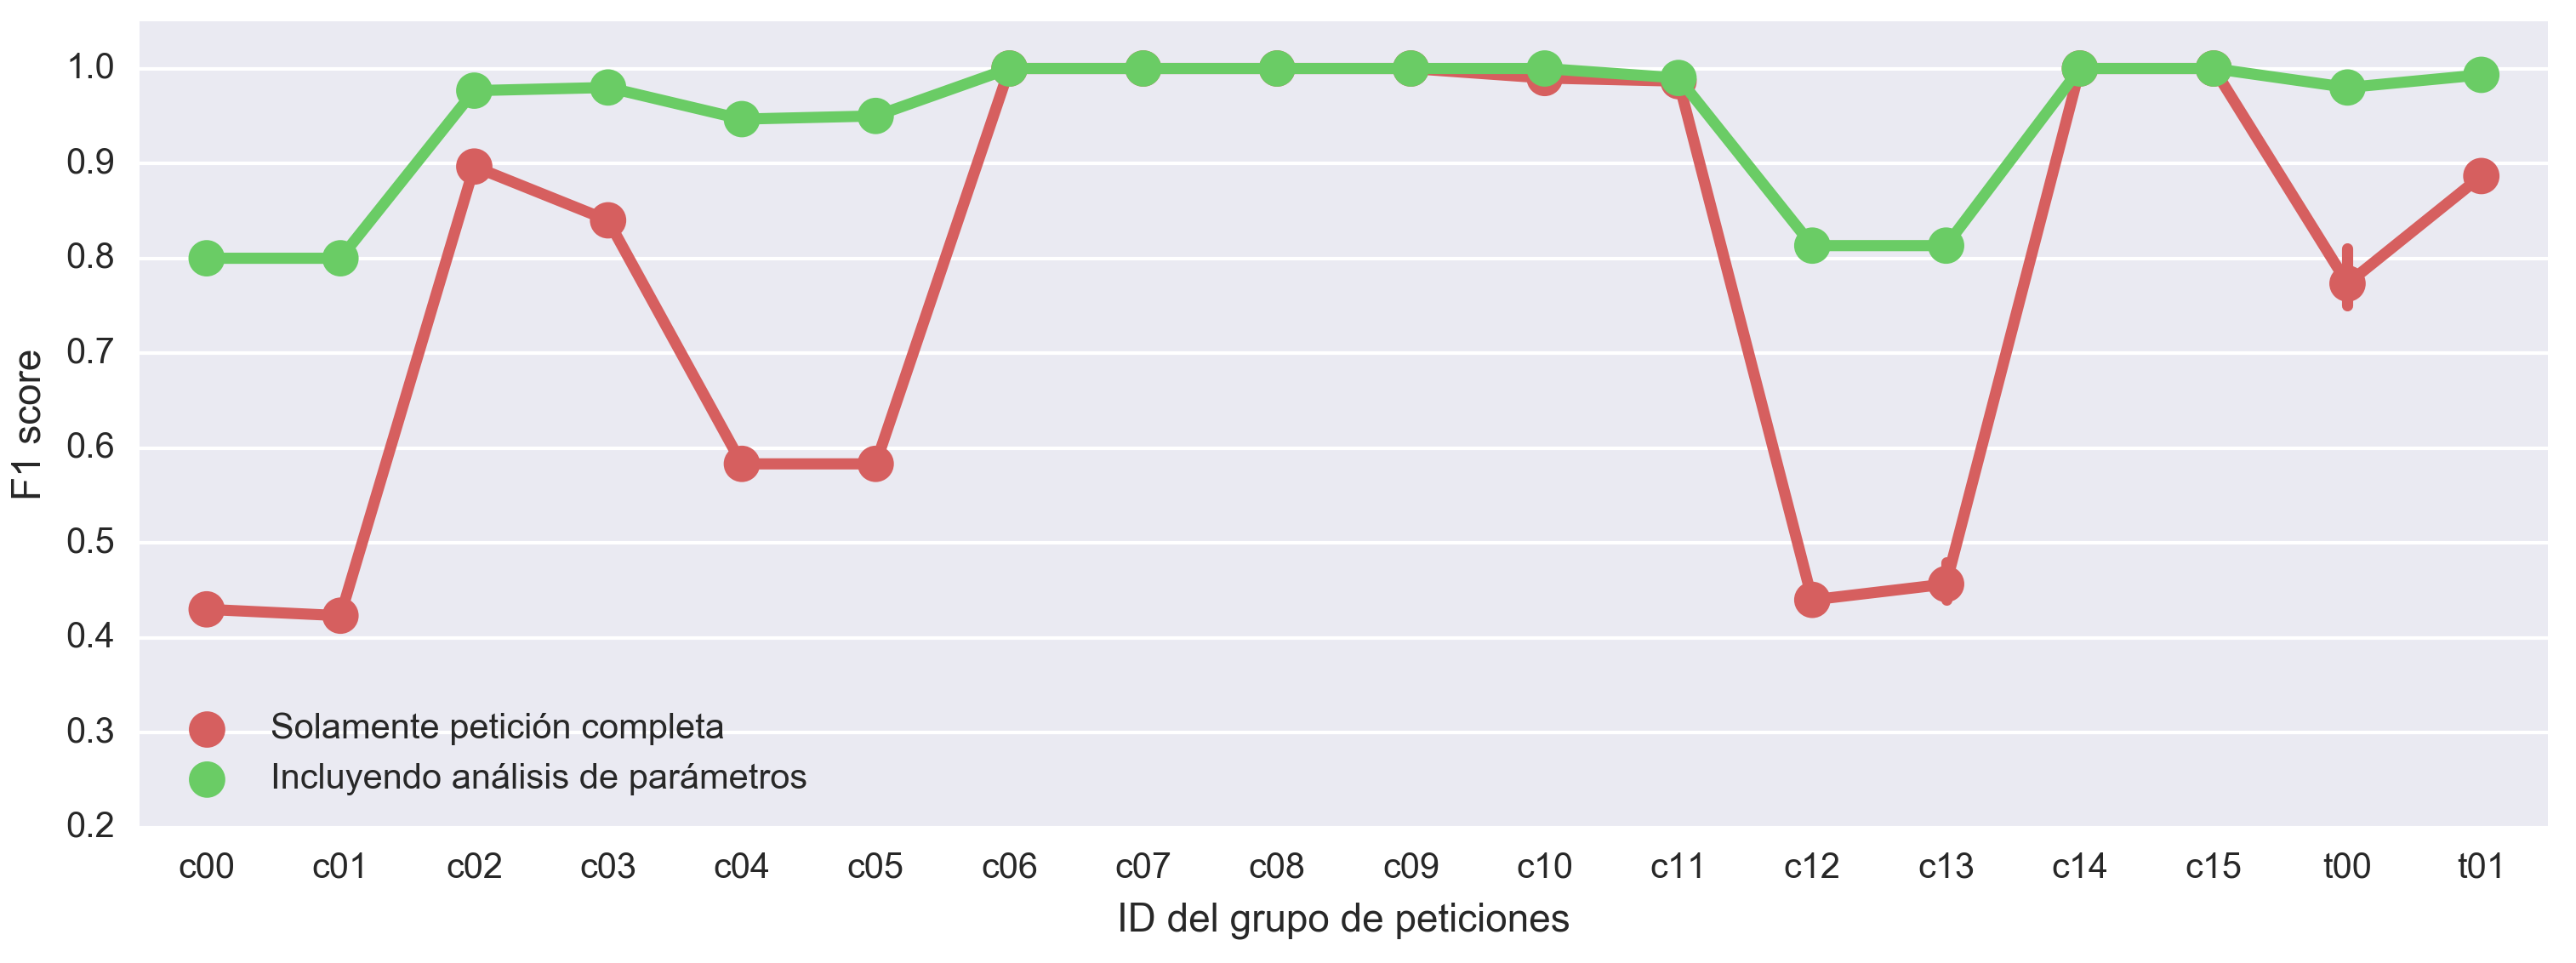
\includegraphics[width=\linewidth]{images/results-features.png}

    \caption{Resultados de detección que muestran las mejoras obtenidas
        con el análisis de valores de parámetros, incluyendo el escalamiento
        de \textit{features}.}
    \label{fig:res:results_features}
\end{figure}

En la \autoref{tbl:res:results_features} y también en la
\autoref{fig:res:results_features} se puede observar los resultados de
la clasificación usando solamente la petición completa, comparado con
los resultados obtenidos incluyendo el análisis de valores de parámetros.
Para ambos casos usamos 1500 peticiones para el entrenamiento de cada
grupo (cerca del 75\% de las muestras) e incluimos el escalamiento de
\textit{features}.
En los resultados promedios de todos los grupos (la última fila de la
tabla) se puede ver que con el análisis de parámetros el \gls{acr3:tpr}
mejora de \num{0.77} a \num{0.93}, el \gls{acr3:fpr} mejora de \num{0.11}
a \num{0.03} y el F$_{1}$-\textit{score} mejora de \num{0.79} a \num{0.95}.

\begin{table}[hbt]
    \centering
    \small
    \begin{tabularx}{\linewidth}{|c|CCC|CCC|}
        \hline
        ID  & \multicolumn{3}{c|}{Solamente petición completa}                                        & \multicolumn{3}{c|}{Incluyendo análisis de parámetros}                                  \\
            & \gls{acr3:tpr}              & \gls{acr3:fpr}              & F$_{1}$-\textit{score}      & \gls{acr3:tpr}              & \gls{acr3:fpr}              & F$_{1}$-\textit{score}      \\
        \specialrule{1.5pt}{0}{0}
        c00 & \num{0.32} $\pm$ \num{0.00} & \num{0.10} $\pm$ \num{0.01} & \num{0.43} $\pm$ \num{0.00} & \num{0.71} $\pm$ \num{0.01} & \num{0.05} $\pm$ \num{0.00} & \num{0.80} $\pm$ \num{0.00} \\ \hline
        c01 & \num{0.31} $\pm$ \num{0.01} & \num{0.10} $\pm$ \num{0.01} & \num{0.42} $\pm$ \num{0.01} & \num{0.72} $\pm$ \num{0.01} & \num{0.05} $\pm$ \num{0.01} & \num{0.80} $\pm$ \num{0.00} \\ \hline
        c02 & \num{0.89} $\pm$ \num{0.03} & \num{0.07} $\pm$ \num{0.05} & \num{0.90} $\pm$ \num{0.01} & \num{1.00} $\pm$ \num{0.00} & \num{0.03} $\pm$ \num{0.01} & \num{0.98} $\pm$ \num{0.01} \\ \hline
        c03 & \num{0.82} $\pm$ \num{0.01} & \num{0.10} $\pm$ \num{0.01} & \num{0.84} $\pm$ \num{0.00} & \num{1.00} $\pm$ \num{0.00} & \num{0.03} $\pm$ \num{0.00} & \num{0.98} $\pm$ \num{0.00} \\ \hline
        c04 & \num{0.83} $\pm$ \num{0.30} & \num{0.70} $\pm$ \num{0.52} & \num{0.58} $\pm$ \num{0.01} & \num{0.91} $\pm$ \num{0.01} & \num{0.01} $\pm$ \num{0.00} & \num{0.95} $\pm$ \num{0.01} \\ \hline
        c05 & \num{0.65} $\pm$ \num{0.30} & \num{0.40} $\pm$ \num{0.52} & \num{0.58} $\pm$ \num{0.01} & \num{0.92} $\pm$ \num{0.01} & \num{0.01} $\pm$ \num{0.00} & \num{0.95} $\pm$ \num{0.00} \\ \hline
        c06 & \num{0.99} $\pm$ \num{0.00} & \num{0.00} $\pm$ \num{0.00} & \num{1.00} $\pm$ \num{0.00} & \num{0.99} $\pm$ \num{0.00} & \num{0.00} $\pm$ \num{0.00} & \num{1.00} $\pm$ \num{0.00} \\ \hline
        c07 & \num{0.99} $\pm$ \num{0.00} & \num{0.00} $\pm$ \num{0.00} & \num{1.00} $\pm$ \num{0.00} & \num{0.99} $\pm$ \num{0.00} & \num{0.00} $\pm$ \num{0.00} & \num{1.00} $\pm$ \num{0.00} \\ \hline
        c08 & \num{1.00} $\pm$ \num{0.00} & \num{0.00} $\pm$ \num{0.00} & \num{1.00} $\pm$ \num{0.00} & \num{1.00} $\pm$ \num{0.00} & \num{0.00} $\pm$ \num{0.00} & \num{1.00} $\pm$ \num{0.00} \\ \hline
        c09 & \num{1.00} $\pm$ \num{0.00} & \num{0.00} $\pm$ \num{0.00} & \num{1.00} $\pm$ \num{0.00} & \num{1.00} $\pm$ \num{0.00} & \num{0.00} $\pm$ \num{0.00} & \num{1.00} $\pm$ \num{0.00} \\ \hline
        c10 & \num{0.99} $\pm$ \num{0.00} & \num{0.01} $\pm$ \num{0.01} & \num{0.99} $\pm$ \num{0.00} & \num{1.00} $\pm$ \num{0.00} & \num{0.00} $\pm$ \num{0.00} & \num{1.00} $\pm$ \num{0.00} \\ \hline
        c11 & \num{0.99} $\pm$ \num{0.01} & \num{0.01} $\pm$ \num{0.01} & \num{0.99} $\pm$ \num{0.01} & \num{1.00} $\pm$ \num{0.00} & \num{0.01} $\pm$ \num{0.00} & \num{0.99} $\pm$ \num{0.00} \\ \hline
        c12 & \num{0.33} $\pm$ \num{0.00} & \num{0.10} $\pm$ \num{0.01} & \num{0.44} $\pm$ \num{0.00} & \num{0.74} $\pm$ \num{0.00} & \num{0.05} $\pm$ \num{0.01} & \num{0.81} $\pm$ \num{0.01} \\ \hline
        c13 & \num{0.35} $\pm$ \num{0.04} & \num{0.13} $\pm$ \num{0.05} & \num{0.46} $\pm$ \num{0.02} & \num{0.74} $\pm$ \num{0.00} & \num{0.05} $\pm$ \num{0.01} & \num{0.81} $\pm$ \num{0.01} \\ \hline
        c14 & \num{1.00} $\pm$ \num{0.00} & \num{0.00} $\pm$ \num{0.00} & \num{1.00} $\pm$ \num{0.00} & \num{1.00} $\pm$ \num{0.00} & \num{0.00} $\pm$ \num{0.00} & \num{1.00} $\pm$ \num{0.00} \\ \hline
        c15 & \num{1.00} $\pm$ \num{0.00} & \num{0.00} $\pm$ \num{0.00} & \num{1.00} $\pm$ \num{0.00} & \num{1.00} $\pm$ \num{0.00} & \num{0.00} $\pm$ \num{0.00} & \num{1.00} $\pm$ \num{0.00} \\ \hline
        t00 & \num{0.67} $\pm$ \num{0.05} & \num{0.10} $\pm$ \num{0.08} & \num{0.77} $\pm$ \num{0.03} & \num{0.99} $\pm$ \num{0.01} & \num{0.06} $\pm$ \num{0.04} & \num{0.98} $\pm$ \num{0.00} \\ \hline
        t01 & \num{0.82} $\pm$ \num{0.01} & \num{0.10} $\pm$ \num{0.01} & \num{0.89} $\pm$ \num{0.01} & \num{1.00} $\pm$ \num{0.00} & \num{0.09} $\pm$ \num{0.06} & \num{0.99} $\pm$ \num{0.01} \\
        \specialrule{1.5pt}{0}{0}
            & \num{0.77} $\pm$ \num{0.28} & \num{0.11} $\pm$ \num{0.22} & \num{0.79} $\pm$ \num{0.23} & \num{0.93} $\pm$ \num{0.11} & \num{0.03} $\pm$ \num{0.03} & \num{0.95} $\pm$ \num{0.08} \\ \hline
    \end{tabularx}

    \caption{Resultados de detección que muestran las mejoras obtenidas
        con el análisis de valores de parámetros, incluyendo el escalamiento
        de \textit{features}.}
    \label{tbl:res:results_features}
\end{table}

De esta forma, los resultados obtenidos muestran la utilidad del análisis
de valores de los parámetros de las peticiones. A parte eso, se puede
notar una reducción de la varianza en las tres métricas, lo que indica
que se redujeron también las diferencias entre los resultados al utilizar
distintos subconjuntos de peticiones para el entrenamiento. Esto es un
indicador de robustez de \gls{acr3:name}, mostrando que con el análisis
de parámetros es menos susceptible a cambios por la elección de peticiones
de entrenamiento.


\subsection{Influencia de la cantidad de peticiones de entrenamiento}

Para que \gls{acr3:name} pueda realizar un buen trabajo de detección,
es necesario que los datos de entrenamiento cubran la mayor cantidad
posible de situaciones que se puedan dar posteriormente en la fase de
detección. Esto puede significar que se tenga que pasar una gran cantidad
de datos al \gls{acr3:waf} para realizar el entrenamiento. Pero el simple
hecho de aumentar la cantidad de peticiones para esta fase no siempre
es la mejor solución, ya que eso aumenta el tiempo que dura la fase de
entrenamiento y además no nos asegura que se cubran realmente todos los
casos normales posibles.

Los conjuntos de datos de prueba que utilizamos nos proveen con \num{2000}
peticiones normales en la mayoría de los grupos, como ya se mostró en la
\autoref{tbl:res:selected_data_sets}. Realizamos una prueba para analizar
los resultados que se obtienen al utilizar distintas cantidades de esos
datos normales para el entrenamiento, siempre incluyendo el escalamiento
de \textit{features} y el análisis de valores de parámetros.

\begin{table}[ht]
    \centering
    \small
    \begin{tabularx}{\linewidth}{|c|CCC|}
        \hline
        Cantidad de peticiones & \multicolumn{3}{c|}{Promedio de los 18 grupos}                                          \\
        de entrenamiento       & \gls{acr3:tpr}              & \gls{acr3:fpr}              & F$_{1}$-\textit{score}      \\
        \specialrule{1.5pt}{0}{0}
        \num{200}              & \num{0.92} $\pm$ \num{0.11} & \num{0.07} $\pm$ \num{0.06} & \num{0.92} $\pm$ \num{0.09} \\ \hline
        \num{500}              & \num{0.94} $\pm$ \num{0.09} & \num{0.06} $\pm$ \num{0.06} & \num{0.93} $\pm$ \num{0.09} \\ \hline
        \num{1000}             & \num{0.93} $\pm$ \num{0.11} & \num{0.03} $\pm$ \num{0.03} & \num{0.94} $\pm$ \num{0.08} \\ \hline
        \num{1500}             & \num{0.93} $\pm$ \num{0.11} & \num{0.03} $\pm$ \num{0.03} & \num{0.95} $\pm$ \num{0.08} \\ \hline
    \end{tabularx}

    \caption{Resultados de detección que muestran la influencia de la
        cantidad de peticiones de entrenamiento, incluyendo el escalamiento
        de \textit{features} y el análisis de valores de parámetros.}
    \label{tbl:res:results_training_samples}
\end{table}

Como se puede observar en la \autoref{tbl:res:results_training_samples},
utilizamos 200, 500, \num{1000} y \num{1500} peticiones para esta prueba,
que equivale a 10\%, 25\%, 50\% y 75\% de los datos disponibles en la
mayoría de los grupos. Los mejores resultados obtuvimos para la mayor
cantidad de peticiones utilizadas, aunque las diferencias comparado a las
demás cantidades son pequeñas y se podría usar también menos peticiones
sin una degradación significativa de la eficacia de detección.
Por esta razón también utilizamos 1500 peticiones para el entrenamiento
en las pruebas presentadas en las secciones anteriores.


\subsection{Influencia de anomalías en los datos de entrenamiento}

Un desafío en ambientes reales es asegurar que los datos de entrenamiento
solamente contengan peticiones \gls{acr3:http} normales y que no haya
ninguna anomalía entre ellas. La presencia de ruido (es decir, anomalías)
en los datos de entrenamiento puede reducir la capacidad de clasificación
del \gls{acr3:ocsvm}, ya que esas anomalías influyen en la posición de
la superficie separadora y consecuentemente esto llevará a resultados
diferentes en la posterior fase de detección.
Como ya presentamos en el capítulo \autoref{chap:p3_concepts_ocsvm}, el
clasificador en cuestión tiene la capacidad de dejar ciertas muestras al
mismo lado del hiperplano que el origen durante la fase de entrenamiento,
de manera que cuenta con cierta capacidad para reducir la influencia de
peticiones anómalas (que son muestras positivas o ataques) que se encuentren
dentro de los datos de entrenamiento. En esta prueba buscamos descubrir
cómo esto se refleja en el desempeño de detección de \gls{acr3:name}.

Realizamos una prueba para analizar en qué manera el \gls{acr3:ocsvm}
se ve afectado en su capacidad de clasificación con la presencia de
peticiones anómalas en los datos de entrenamiento. Para eso, incluimos
una cierta cantidad de anomalías dentro de las peticiones de entrenamiento
para llegar a 1\%, 5\% y 10\% de anomalías. Acá volvimos a utilizar 200,
500, \num{1000} y \num{1500} peticiones para el entrenamiento, siempre
incluyendo el escalamiento de \textit{features} y el análisis de valores
de parámetros.

\begin{figure}[ht]
    \centering
    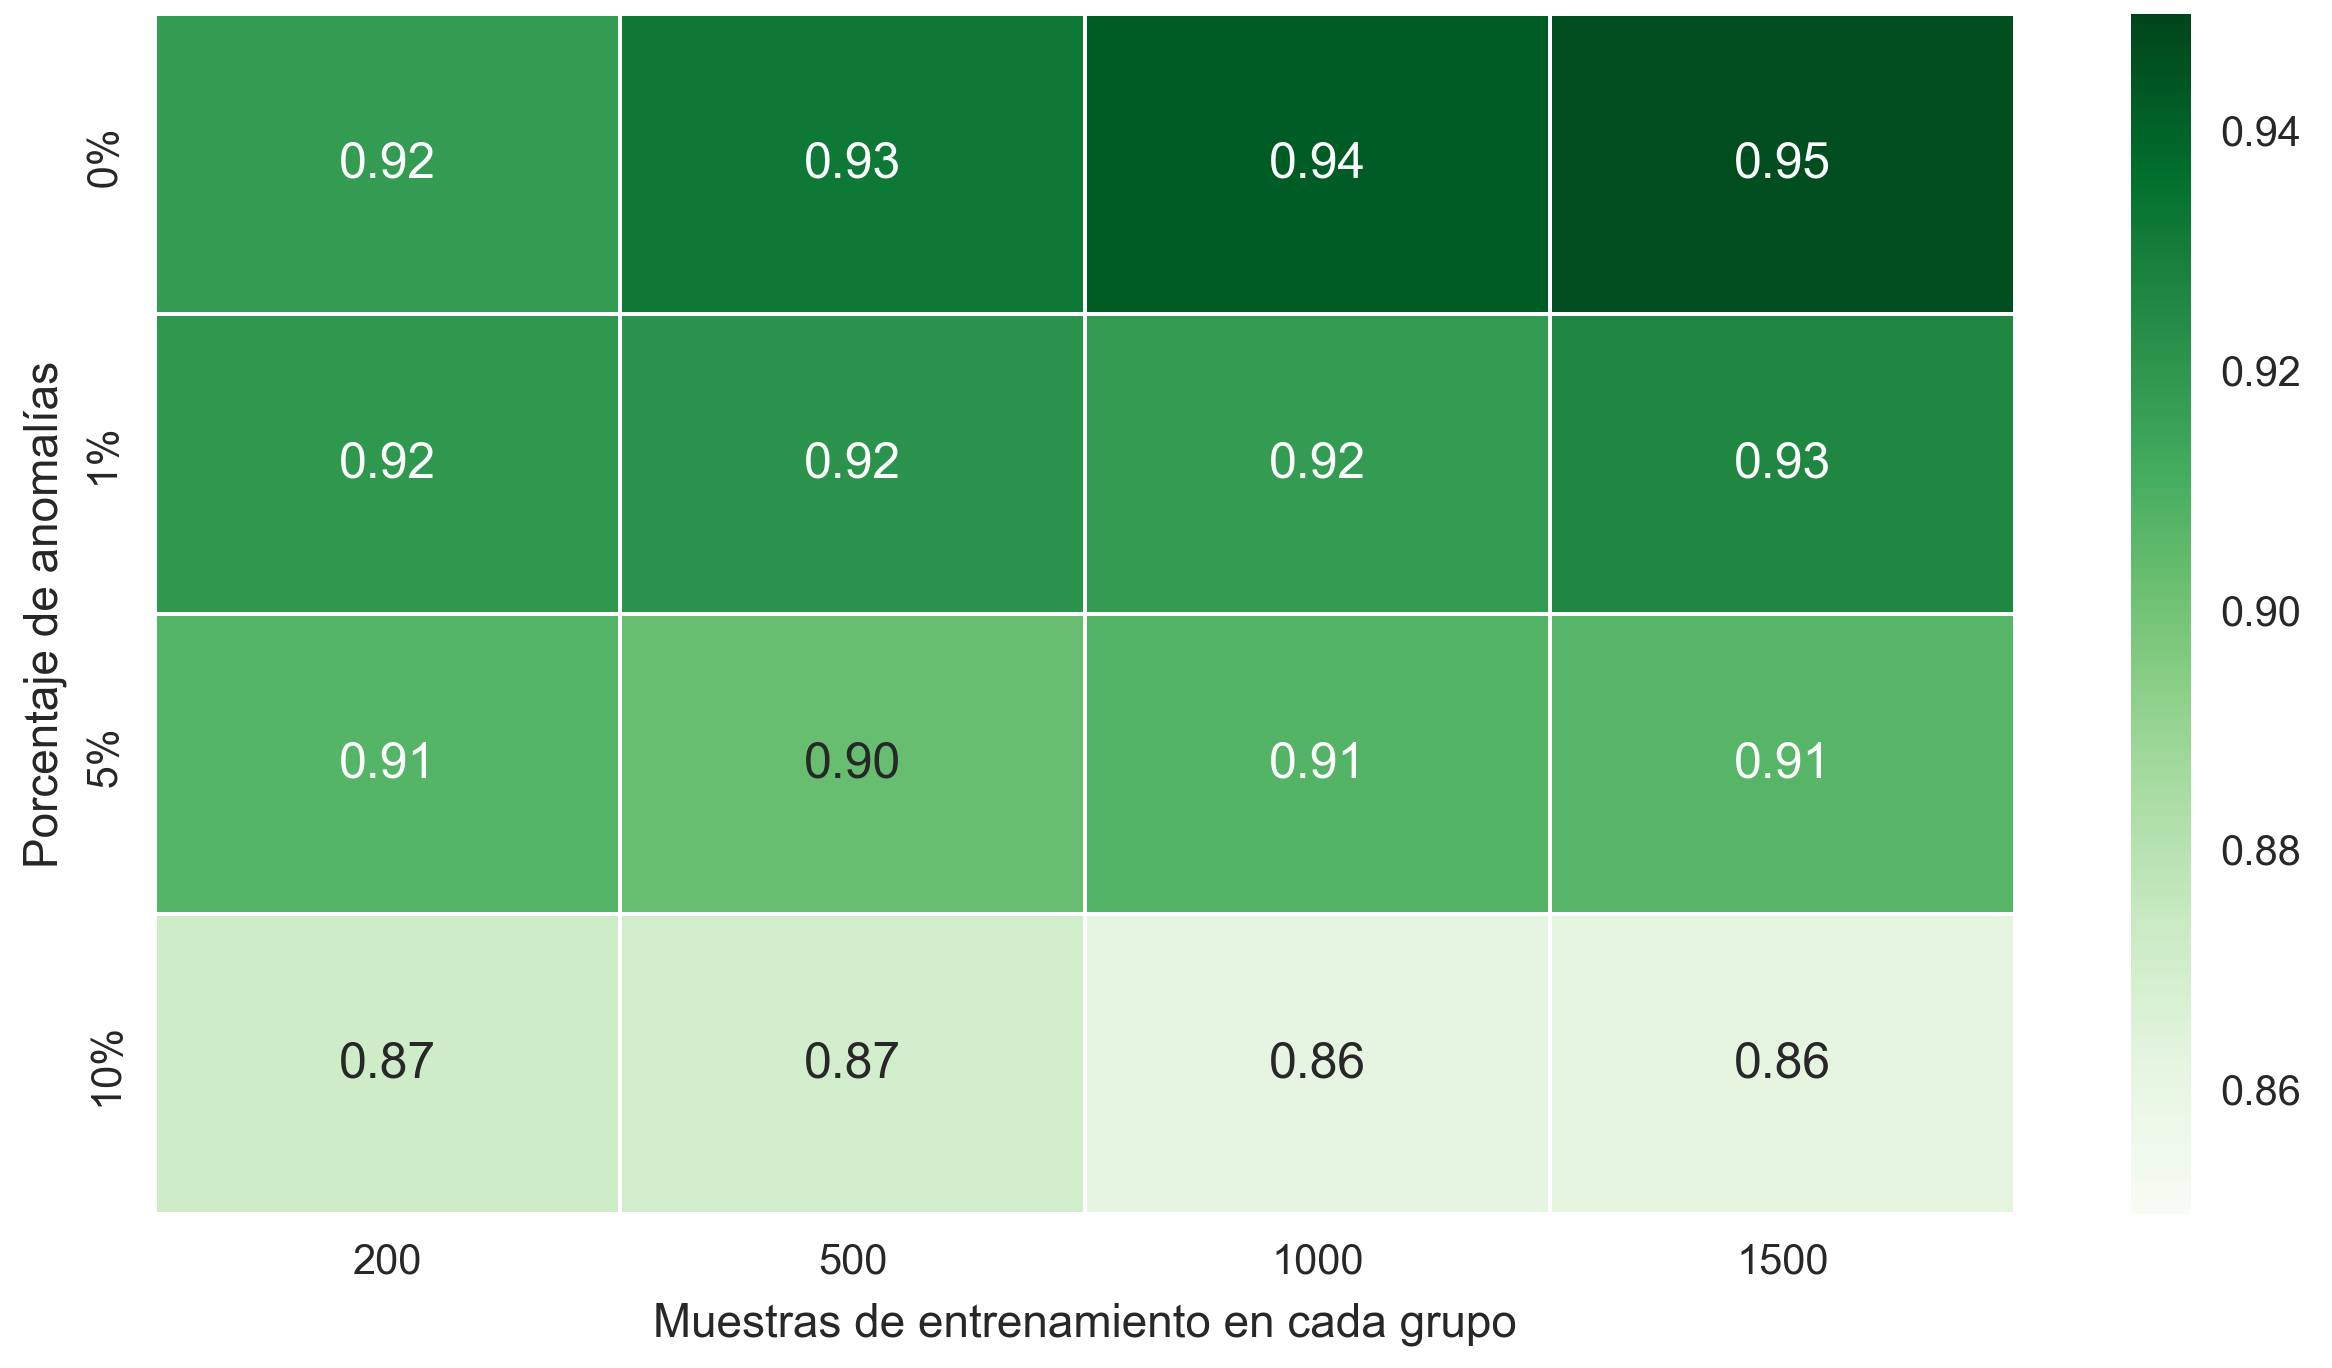
\includegraphics[width=\linewidth]{images/results-training-anomalies.png}

    \caption{Mapa de calor de los resultados de detección, en términos
        del F$_{1}$-\textit{score}, que muestran la influencia de la
        cantidad de peticiones y el porcentaje de anomalías en el
        entrenamiento, incluyendo el escalamiento de \textit{features}
        y el análisis de valores de parámetros.}
    \label{fig:res:results_training_anomalies}
\end{figure}

La \autoref{fig:res:results_training_anomalies} muestra un mapa de calor
(\textit{heatmap}) de los resultados de detección de esta prueba. Las
columnas contienen las distintas cantidad de peticiones utilizadas para
el entrenamiento, las filas representan diferentes porcentajes de anomalías
que se incluyeron en los datos de entrenamiento y los valores en cada celda
indican el F$_{1}$-\textit{score} promedio de los 18 grupos que se obtuvo
con esa configuración. Las celdas con colores más oscuros contienen
números mayores, lo que indica resultados mejores.

Como se puede ver en nuestros resultados, el F$_{1}$-\textit{score} sufre
una degradación gradual conforme va aumentando el porcentaje de anomalías,
aunque es una reducción poco significativa para 1\% de anomalías.
Esta degradación de la detección se da de forma similar para todas las
cantidad de peticiones utilizadas para el entrenamiento, aunque el caso
más pronunciado se da para la mayor cantidad de peticiones. Esto se debe
a que ya se tiene mayor cantidad de anomalías presentes, por ejemplo
con 10\% de \num{1500} peticiones ya hay 150 muestras anómalas que ejercen
influencia sobre la posición y forma de la superficie separadora de los
clasificadores, lo que se ve reflejado en los resultados.

Cabe resaltar que un 10\% de anomalías de entrenamiento ya es un porcentaje
muy elevado de ruido. En ese caso se debería utilizar alguna estrategia
adicional para obtener un conjunto de datos de entrenamiento más limpio,
como por ejemplo una clasificación previa con aprendizaje no supervisado,
con el fin de reducir el impacto negativo sobre la eficacia de detección
del \gls{acr3:waf}.

De esta forma, los resultados obtenidos en esta prueba muestran que
\gls{acr3:name} con sus clasificadores \gls{acr3:ocsvm} presenta cierta
robustez frente a la presencia de algunas pocas anomalías en los datos
de entrenamiento.


\section{Análisis del tiempo de respuesta de las aplicaciones protegidas}

Esta prueba que realizamos con \gls{acr3:name} apunta a cuantificar en
qué medida se ve afectado el tiempo de respuesta de las aplicaciones web
que nuestra implementación debe proteger.
Si este tiempo de respuesta aumenta de gran manera debido al uso del
\gls{acr3:waf}, las aplicaciones podrían quedar inutilizables para el
usuario final, significando que nuestra implementación no puede ser
usada para detección en tiempo real.
Estamos conscientes de que las mediciones realizadas durante esta prueba
no necesariamente reflejan un ambiente real, pero sí nos permiten establecer
el orden de magnitud de la variación que introduce \gls{acr3:name} en
el tiempo de respuesta de las aplicaciones protegidas.

Para esta prueba, nosotros creamos una simple aplicación capaz de recibir
peticiones \gls{acr3:http} y enviar las respuestas correspondientes, con
el fin de simular aplicaciones web protegidas por \gls{acr3:name}.
Posteriormente medimos el intervalo de tiempo entre el envío de una petición
a esa aplicación y la recepción de la respuesta.
Realizamos esta medición con tres configuraciones distintas. En la primera
configuración se enviaron las peticiones directamente a la aplicación
destino sin pasar por \gls{acr3:name}, para obtener así el tiempo de
respuesta normal. En la segunda configuración el tráfico fue enviado a
través del \gls{acr3:waf} pero sin que este realice las tareas de detección,
para de esta manera medir el retraso incurrido por agregar un componente
al camino de los paquetes. En la última configuración las peticiones
pasaron por un \gls{acr3:waf} previamente entrenado, con el fin de medir
el retraso ocasionado al utilizar las funciones de detección.

El código de todas las partes utilizadas en esta prueba esta en nuestro
repositorio público, en el directorio \path{/tests/waf_speed/}. Ejecutamos
todos los procesos en una misma máquina, buscando reducir de esta manera
diferentes variables presentes en la red y concentrarnos en el retraso
introducido por el uso del \gls{acr3:waf}.
La máquina utilizada tiene una plataforma \textit{Ubuntu 14.04} de 64
\textit{bits}, con un procesador \textit{Intel i5} de \num{1.7} \gls{acr3:ghz}
y 8 \gls{acr3:gb} de memoria \gls{acr3:ram}.

\begin{table}[ht]
    \centering
    \small
    \begin{tabularx}{\linewidth}{|l|C|}
        \hline
        \multicolumn{1}{|c|}{Configuración}   & Tiempo de respuesta promedio (milisegundos) \\
        \specialrule{1.5pt}{0}{0}
        Sin \gls{acr3:waf}                    &  \num{4.8} $\pm$ \num{2.2} \\ \hline
        Con \gls{acr3:waf} pero sin detección &  \num{6.4} $\pm$ \num{1.7} \\ \hline
        Con \gls{acr3:waf} y con detección    & \num{10.1} $\pm$ \num{2.6} \\ \hline
    \end{tabularx}

    \caption{Resultados de la prueba de tiempo de respuesta de las
        aplicaciones protegidas.}
    \label{tbl:res:test_2}
\end{table}

En la \autoref{tbl:res:test_2} se pueden ver los resultados de esta
prueba. Para cada una de las tres configuraciones cronometramos 160
peticiones pertenecientes a distintos grupos de método y \gls{acr3:url},
de las cuales la mitad fueron peticiones normales y la otra mitad anomalías.
No pudimos percibir diferencias significativas de tiempo entre peticiones
normales y anómalas, ni tampoco entre peticiones de distintos grupos
(con distintas cantidades de parámetros). Posibles variaciones están
contenidas dentro de la desviación estándar indicada en la tabla mencionada.
Los resultados se mantuvieron constantes en repeticiones de la misma prueba.

La configuración sin \gls{acr3:name} obtuvo el menor tiempo de respuesta,
con un promedio de \num{4.8} milisegundos.
En la segunda configuración, que utiliza \gls{acr3:name} sin detección,
se obtuvo un retardo adicional de \num{1.6} milisegundos en tiempo de
respuesta comparado al primer caso. La tercera configuración, que incluye
la detección, obtuvo retardos adicionales de \num{5.3} y \num{3.7}
milisegundos comparado con las dos primeras configuraciones respectivamente.
Esto indica el orden de magnitud del retraso que \gls{acr3:name} podría
agregar a las peticiones. Se espera que esto sea un límite superior
para un \gls{acr3:waf} optimizado (incluso utilizando otro lenguaje).

Además, considerando que la latencia promedio de paquetes de red en
Internet está entre 200 y 300 milisegundos \citep{internetWeatherMap}
y será un poco mayor a eso para mensajes \gls{acr3:http}, se espera que
estos pocos milisegundos adicionales agregados por \gls{acr3:name} no
afectarán de forma notable el tiempo de respuesta de las aplicaciones
web protegidas.
Para aplicaciones dentro de una red interna de alta velocidad, el retraso
podría llegar a ser perceptible, pero nuestra implementación fue hecha
en primer lugar para aplicaciones accesibles a través de Internet, como
fue explicado en la introducción en el \autoref{chap:p3_introduction}.


\section{Análisis del tiempo de entrenamiento}

En esta última prueba realizada se analizó la relación que existe entre
el tiempo de entrenamiento de \gls{acr3:name} (que incluye el tiempo
consumido por los procesos de extracción de \textit{features} y los
clasificadores \gls{acr3:ocsvm} empleados) y la cantidad de peticiones
\gls{acr3:http} utilizadas para dicho entrenamiento.

La duración estimada del entrenamiento es una información importante
para los administradores responsables por \gls{acr3:name}, ya que estas
personas necesitan saber si el entrenamiento durará minutos, horas o días,
a fin de poder planificar los momentos adecuados para este proceso.
De la misma manera que en la prueba anterior, estamos conscientes de que
las mediciones realizadas durante esta prueba no necesariamente reflejan
un ambiente real con un \gls{acr3:waf} optimizado (incluso utilizando otro
lenguaje de programación), pero sí nos permiten establecer el orden de
magnitud del tiempo de entrenamiento de nuestra implementación y la relación
entre este tiempo y la cantidad de peticiones que fueron utilizadas.

El código para esta prueba también esta en nuestro repositorio público,
en el directorio \path{/tests/training_duration/}.
Volvimos a utilizar la misma máquina para ejecutar las pruebas, que tiene
una plataforma \textit{Ubuntu 14.04} de 64 \textit{bits}, con un procesador
\textit{Intel i5} de \num{1.7} \gls{acr3:ghz} y 8 \gls{acr3:gb} de memoria
\gls{acr3:ram}.

\begin{table}[ht]
    \centering
    \small
    \begin{tabularx}{\linewidth}{|r|C|C|r|}
        \hline
        \multicolumn{1}{|c|}{\begin{tabular}[c]{@{}c@{}}Cantidad de\\ peticiones\end{tabular}}
        & \multicolumn{1}{c|}{\begin{tabular}[c]{@{}c@{}}Tiempo promedio\\ por petición (segundos)\end{tabular}}
        & \multicolumn{1}{c|}{\begin{tabular}[c]{@{}c@{}}Tiempo máximo\\ por petición (segundos)\end{tabular}}
        & \multicolumn{1}{c|}{\begin{tabular}[c]{@{}c@{}}Tiempo total\\ máximo (segundos)\end{tabular}} \\
        \specialrule{1.5pt}{0}{0}
        \num{10}     & \num{0.0013} $\pm$ \num{0.0004} & \num{0.0020} &   \num{0.0195} \\ \hline
        \num{100}    & \num{0.0011} $\pm$ \num{0.0004} & \num{0.0017} &   \num{0.1724} \\ \hline
        \num{1000}   & \num{0.0010} $\pm$ \num{0.0004} & \num{0.0017} &   \num{1.7126} \\ \hline
        \num{10000}  & \num{0.0011} $\pm$ \num{0.0004} & \num{0.0018} &  \num{17.9132} \\ \hline
        \num{100000} & \num{0.0020} $\pm$ \num{0.0005} & \num{0.0070} & \num{703.9531} \\ \hline
    \end{tabularx}

    \caption{Resultados de la prueba de tiempo de entrenamiento.}
    \label{tbl:res:test_3}
\end{table}

La \autoref{tbl:res:test_3} muestra los resultados de esta prueba, indicando
el tiempo por petición que se alcanzó para las diferentes cantidades
utilizadas para el entrenamiento. Para cada una de estas cantidades,
realizamos entrenamientos con cada uno los grupos de \gls{acr3:url} y
método \gls{acr3:http}.
Cabe mencionar que el tiempo de entrenamiento de cada clasificador está
influenciado por la cantidad de \textit{features} extraídos en cada uno
de estos grupos de peticiones y debido a esto el tiempo medido puede ser
diferente para cada grupo. La tabla de resultados muestra el tiempo
promedio y también el tiempo máximo; este último puede ser utilizada a
modo de establecer un límite superior de la duración del entrenamiento.

En la tabla mencionada podemos observar que el tiempo de entrenamiento
máximo está en el orden de algunos milisegundos por petición, específicamente
el máximo está en 7 milisegundos. Esto significa que el entrenamiento
de \gls{acr3:name} puede tardar unos 704 segundos (cerca de 12 minutos)
para una cantidad de \num{100000} peticiones.
En nuestra opinión, este tiempo es muy manejable, permitiendo que el
\gls{acr3:waf} pueda ser entrenado con nuevos datos en cuestión de
minutos en los momentos que el administrador del mismo lo considere
necesario.


\section{Comparación con trabajos relacionados}

En esta sección queremos comparar nuestro implementación y los resultados
que obtuvimos con algunos trabajos de autores relacionados al área de
\gls{acr3:ids} con detección de anomalías. Nos enfocamos en trabajos que
utilizan los mismos conjuntos de datos que nosotros empleamos. En la
\autoref{tbl:res:comparison} se muestra un resumen de la comparación de
resultados de nuestra implementación con trabajos de otros investigadores.

\begin{table}[ht]
    \centering
    \small
    \begin{tabularx}{\linewidth}{|l|X|c|c|c|}
        \hline
        \multicolumn{1}{|c|}{Sistema de detección} & \multicolumn{1}{c|}{Observaciones}         & \gls{acr3:tpr} & \gls{acr3:fpr} & F$_{1}$-\textit{score} \\
        \specialrule{1.5pt}{0}{0}
        \gls{acr3:name}                            & \gls{acr3:ocsvm}s con cantidad variable de & \num{0.93}     & \num{0.03}     & \num{0.95}             \\
        (el presente trabajo)                      & \textit{features}                          &                &                &                        \\ \hline
        \textit{ModSecurity}                       & popular detector por firmas de ataques     & \num{0.56}     & \num{0.00}     & \num{0.71}             \\
        \citep{gimenez2015tfg}                     &                                            &                &                &                        \\ \hline
        \textit{HTTP-WS-AD}                        & modelos estadísticos con agregación y      & \num{0.99}     & \num{0.02}     & \num{0.99}             \\
        \citep{gimenez2015tfg}                     & cascada                                    &                &                &                        \\ \hline
        \citep{torranoGimenez2015study}            & promedio de cuatro tipos distintos de      & \num{0.95}     & \num{0.05}     & -                      \\
                                                   & árboles de decisión                        &                &                &                        \\ \hline
        \textit{OC-WAD}                            & conjunto de \gls{acr3:ocsvm}s con          & \num{0.96}     & \num{0.03}     & -                      \\
        \citep{parhizkar2015oc}                    & cantidad fija de \textit{features}         &                &                &                        \\ \hline
    \end{tabularx}

    \caption{Comparación de resultados de \gls{acr3:name} con otros trabajos
        que utilizan también el conjunto de datos \gls{acr3:csic} 2010.}
    \label{tbl:res:comparison}
\end{table}

Antes de analizar otras propuestas de detección de anomalías, investigamos
sobre \gls{acr3:ids} basados en firmas de ataques (no realizan detección
de anomalías) para tener una referencia sobre este tipo de sistemas de
detección. Una implementación popular de un \gls{acr3:waf} basados en
firmas es \textit{ModSecurity}.
En \citep{gimenez2015tfg} % from section 5.3.2 - tabla 5.25 CSIC-ModSecurity
el autor aplicó este detector al conjunto de datos \gls{acr3:csic} 2010,
utilizando las firmas de ataques que el mismo trae por defecto. Así obtuvo
un \gls{acr3:tpr} de \num{0.56}, un \gls{acr3:fpr} de \num{0.00} y un
F$_{1}$-\textit{score} de \num{0.71}. Una fortaleza de este detector es que
no incurre en falsos positivos (peticiones normales detectadas como ataques).
Pero nuestra implementación obtiene una detección significativamente mejor
que este popular detector basado en firmas de ataques, como se puede ver
en los resultados de la ya mencionada \autoref{tbl:res:comparison}.

En \citep{gimenez2015tfg} % from section 6.1.6 - conclusiones
se presenta un detector de anomalías llamado \textit{HTTP-WS-AD}.
En este trabajo se utilizan varios modelos estadísticos y se realizan
pruebas con varios esquemas de agregación y cascada de modelos para
mejorar los resultados de la detección de peticiones \gls{acr3:http}
anómalas. El autor reporta haber obtenido un \gls{acr3:tpr} de \num{0.99},
un \gls{acr3:fpr} de \num{0.02} y un F$_{1}$-\textit{score} de \num{0.99}
para el conjunto de datos \gls{acr3:csic} 2010.
Cada una de estos tres resultados es levemente superior a los números
logrados por \gls{acr3:name}, con la notable diferencia de que este
trabajo utiliza métodos estadísticos mientras que nuestra implementación
emplea herramientas del área de \gls{acr3:ml}.
Además, Giménez también realizó mediciones del impacto de su detector
en el tiempo de respuesta de las aplicaciones web protegidas, reportando
un retraso adicional promedio de 50 milisegundos introducido por las tareas
de detección. % from table 5.27 - CSIC-Medición de Tiempos de Respuesta
\gls{acr3:name} obtuvo un retraso promedio menor a 10 milisegundos en
nuestras pruebas, mostrando una leve ventaja en este aspecto frente a
\textit{HTTP-WS-AD}.

En la segunda parte del trabajo
\citep{torranoGimenez2015study} % from section 6.2 - second point in conclusions
se presenta un detector de anomalías que utiliza cuatro tipos de árboles
de decisiones para su proceso de detección. Estos árboles son también
herramientas de clasificación del área de \gls{acr3:ml}, pero en este
caso se trata de clasificadores binarios o de dos clases. Esto significa
que se entrena los clasificadores con peticiones normales y anómalas.
El trabajo en cuestión reporta haber obtenido un \gls{acr3:tpr} de \num{0.95}
y un \gls{acr3:fpr} de \num{0.05} sobre el conjunto de datos \gls{acr3:csic}
2010. \gls{acr3:name} obtuvo un \gls{acr3:tpr} inferior con \num{0.93},
pero obtuvo un \gls{acr3:fpr} superior de \num{0.03}.
Cabe resaltar que el trabajo en cuestión entrena sus clasificadores con
ambas clases de peticiones (normales y anomalías), mientras que nosotros
entrenamos con peticiones normales únicamente. Creemos que debido a eso,
\gls{acr3:name} es más robusto frente a la aparición de nuevos tipos de
ataques, ya que no se usan anomalías en el entrenamiento.

En \citep{parhizkar2015oc} % from section VI - conclusions
se presenta un detector de anomalías llamado \textit{OC-WAD} para peticiones
\gls{acr3:http}. Los autores extraen una cantidad fija de \textit{features}
de las peticiones y posteriormente utilizan un conjunto de clasificadores
\gls{acr3:ocsvm} con \textit{kernel} \gls{acr3:rbf} para realizar la
detección. Los distintos clasificadores son entrenados con diferentes
subconjuntos de \textit{features}. Además, ellos presentan un algoritmo
de enjambres llamado \textit{BeeSnips}, que utilizan para la creación
y optimización del conjunto de clasificadores.
Trabajando con el conjunto de datos \gls{acr3:csic} 2010, los autores
reportan haber obtenido un \gls{acr3:tpr} de \num{0.96} y un \gls{acr3:fpr}
de \num{0.03}. Estos resultados son similares a los nuestros; obtuvimos
un \gls{acr3:tpr} inferior de \num{0.93} y un \gls{acr3:fpr} igual de
\num{0.03}. Pero en este trabajo nos se brinda mucha información sobre
la manera que realizaron sus pruebas; por ejemplo no explican si entrenan
conjuntos de clasificadores separados por \gls{acr3:url}, lo que nos
deja dudas sobre cuan comparables son nuestros resultados.

    \renewcommand{\newCommandChapterTitle}{Conclusiones}
\chapter{\newCommandChapterTitle}
\markright{\hfill \thechapter. \newCommandChapterTitle}
\label{chap:p3_conclusions}


En este capítulo presentamos las conclusiones de nuestro trabajo.
Primeramente damos un resumen general del contenido que fue presentado
a lo largo de este trabajo, incluyendo el análisis de los resultados
que obtuvimos en las pruebas realizadas con el detector \gls{acr3:name}.
Después mostramos de qué forma hemos logrado alcanzar los objetivos que
nos propusimos para esta investigación. Finalmente, concluimos este
trabajo describiendo varios aspectos de nuestra implementación en los
cuales pueden realizarse mejoras; estos aspectos podrían dar lugar a
trabajos futuros.


\section{Resumen de la investigación}

En esta sección presentamos los aspectos más importantes que fueron
descritos en cada uno de los capítulos anteriores, buscando brindar de
esta forma un resumen de las ideas principales de este trabajo.

En el \autoref{chap:p3_introduction} introducimos el tema de este trabajo.
Describimos el área de estudio que rodea nuestra investigación, que abarca
el área de \gls{acr3:ids} con detección de anomalías, características
de los mensajes \gls{acr3:http} y también la herramienta \gls{acr3:ocsvm}
del área de \gls{acr3:ml}. Luego mostramos la problemática que nos llevó
a realizar este trabajo, argumentando que vulnerabilidades presentes en
muchas aplicaciones web presentan un gran riesgo y se necesita mecanismos
para protegerlos. Al final de ese capítulo presentamos los objetivos que
nos hemos propuesto para este trabajo de investigación; estos objetivos
se centran en la detección de mensajes \gls{acr3:http} anómalos mediante
un \gls{acr3:waf} basado en detección de anomalías, utilizando clasificadores
\gls{acr3:ocsvm}, con el fin de mitigar los riesgos existentes de ataques
contra aplicaciones web a través de la Internet.

En el \autoref{chap:p3_concepts_features} presentamos nuestros procesos
de extracción de \textit{features}. Estos procesos se basan de gran manera
en los aportes de los trabajos de Kruegel y Vigna, especialmente en la
manera como aprovechan las características de mensajes \gls{acr3:http}
para proponer sus modelos de anomalías. Luego explicamos los procesos que
diseñamos, incluyendo el análisis de valores de parámetros que realizamos
y cada uno de los \textit{features} que extraemos de esos valores para
representar las características de los mensajes como vectores numéricos.
Estos vectores pueden tener longitudes distintas según el grupo de método
\gls{acr3:http} y \gls{acr3:url} al que pertenecen, ya que esto depende
de la cantidad de parámetros de las peticiones.
Las características analizadas de las peticiones son la distribución de
caracteres, la entropía y la cantidad de caracteres. Se complementa esta
extracción de \textit{features} con un proceso de escalamiento para reducir
el impacto de los distintos rangos de números que pueden tener los diferentes
\textit{features}.

En el \autoref{chap:p3_concepts_ocsvm} describimos en detalle el
clasificador \gls{acr3:ocsvm}, que constituye la parte central de nuestro
\gls{acr3:waf}. Una de las ventajas de utilizar este clasificador es que
no necesitamos peticiones anómalas para el entrenamiento, reduciendo así
el impacto que tiene la aparición de nuevos tipos de ataques; solamente
se vuelve a realizar el entrenamiento cuando haya cambios en las aplicaciones
protegidas.
Mostramos que se utiliza vectores de \textit{features} que representan
a las peticiones de entrenamiento para trazar un hiperplano que separa
este grupo de entrenamiento del origen. Posteriormente, en la fase de
detección, se determina a qué lado del hiperplano pertenecen los vectores
de las nuevas peticiones, para así determinar si corresponden a peticiones
normales o anómalas.
La selección de valores de los parámetros \gls{sim3:nui} y \gls{sim3:gammai}
del clasificador se realizó de forma experimental para los conjuntos de
datos utilizados y creemos que esto no variará mucho para conjuntos de
datos diferentes.

El \autoref{chap:p3_new_waf} detalla la implementación y funcionamiento
de \gls{acr3:name} que fue construido en el marco de este trabajo.
Describimos los detalles de la implementación, incluyendo los pasos
intermedios de cada una de las dos fases, que son las fases de entrenamiento
y detección. Se explicaron las particularidades de nuestra implementación,
detallando también los componentes externos y librerías que utilizamos.
El código fuente de la implementación está disponible en un repositorio
público bajo la dirección \TheRepoUrl.

El \autoref{chap:p3_results} presenta las pruebas realizadas con nuestra
implementación y expone los resultados obtenidos en cada una de ellas.
Utilizamos los conjuntos de datos \gls{acr3:csic} 2010 \citep{csic2010dataset}
y \gls{acr3:csic} TORPEDA 2012 \citep{torpeda2012dataset}, que contienen
peticiones \gls{acr3:http} hechas a una aplicación de comercio electrónico.
Las pruebas experimentales analizaron tres características de \gls{acr3:name}:
la eficacia de detección, el impacto en el tiempo de respuesta de las
aplicaciones protegidas y el tiempo de entrenamiento.

Analizando la primera de estas característica, la eficacia de detección
de \gls{acr3:name}, logramos obtener un \gls{acr3:tpr} de \num{0.93},
un \gls{acr3:fpr} de \num{0.03} y un F$_{1}$-\textit{score} de \num{0.95}.
Estos son resultados promedios para los 18 grupos de peticiones que
utilizamos de los conjuntos de datos.
Empleamos el escalamiento de \textit{features} e incluimos el análisis
de valores de parámetros en las peticiones, ya que utilizando estas dos
estrategias obtuvimos los mejores resultados. Además, realizamos el
entrenamiento con 1500 peticiones en cada grupo (cerca del 75\% de las
muestras normales), atendiendo a que no haya anomalías en los datos de
entrenamiento.
Notamos que el \gls{acr3:tpr} promedio alcanzado de \num{0.93} es algo
bajo; inspeccionando los grupos individuales descubrimos que la mayoría
tiene un \gls{acr3:tpr} mayor o igual a \num{0.99}, pero cuatro grupos
alcanzan solamente un \gls{acr3:tpr} alrededor de \num{0.72}. Estos cuatro
grupos justamente son los que tienen la mayor cantidad de parámetros (y
por lo tanto la mayor cantidad de \textit{features}), y esto podría indicar
que nuestro \gls{acr3:waf} tiene dificultades con peticiones que tienen
muchos parámetros.

En la segunda característica analizada mediante las pruebas, tratamos
de cuantificar el impacto que nuestro \gls{acr3:waf} podría tener sobre
el tiempo de respuesta de las aplicaciones web que protege. A pesar de
que nuestra implementación puede ser optimizada, logramos que el retraso
adicional en el tiempo de repuesta sea despreciable comparado con la
latencia promedio del tráfico de red en Internet, por lo que el trabajo
de detección de nuestro \gls{acr3:waf} no afectaría de forma notable
el tiempo de respuesta de las aplicaciones protegidas.

En la tercera característica analizada mediante las pruebas, que trata
del tiempo de entrenamiento de nuestro \gls{acr3:waf}, verificamos que
esta duración depende de la cantidad de peticiones utilizadas para dicha
fase de entrenamiento. Los números indican que se puede entrenar nuestra
implementación con \num{100000} peticiones en alrededor de 12 minutos.
Esta rapidez le provee mucha flexibilidad a los administradores del
\gls{acr3:waf} para poder planificar los momentos de entrenamiento.
Recordamos que el entrenamiento solamente es necesario después de realizar
cambios en las aplicaciones protegidas, y la eficacia de detección del
sistema no debería verse afectada por la aparición de nuevos ataques.

Al final del \autoref{chap:p3_results} realizamos también una comparación
de \gls{acr3:name} con propuestas de otros trabajos del área. Para poder
comparar los resultados, nos enfocamos en aquellos que utilizan el mismo
conjunto de datos que nosotros empleamos para las pruebas. Analizamos
propuestas que utilizan distintas herramientas, como por ejemplo árboles
de decisión, modelos estadísticos y también el mismo clasificador
\gls{acr3:ocsvm}.


\section{Alcance de los objetivos}

En esta parte volvemos a presentar los objetivos que nos habíamos propuesto
en el \autoref{chap:p3_introduction} y mostramos de qué manera logramos
alcanzar los mismos a través del trabajo realizado a lo largo de esta
investigación. Empezamos describiendo nuestros logros para los objetivos
específicos, para después cerrar con el objetivo general.


\subsection{Objetivos específicos}

\begin{enumerate}
    \item
    Diseñar procesos de extracción de características (\textit{features})
    específicamente para mensajes \gls{acr3:http}, basado en aportes de
    otros investigadores de la literatura.

    \begin{itemize}
        \item
        Partiendo de los trabajos de los autores Kruegel y Vigna, y
        combinando sus aportes con trabajos de la literatura especializada,
        se diseñó procesos de extracción de \textit{features} que pueden
        representar características de los mensajes \gls{acr3:http}
        mediante vectores de \textit{features} numéricos.
        Estos procesos de extracción fueron descritos en el
        \autoref{chap:p3_concepts_features}, mientras que en el
        \autoref{chap:p3_new_waf} se mostraron los detalles de la
        implementación de los mismos.
        Las pruebas experimentales presentadas en el \autoref{chap:p3_results}
        demuestran la utilidad de estos procesos diseñados para la tarea
        de detección de anomalías en mensajes \gls{acr3:http}.
    \end{itemize}

    \item
    Implementar un \gls{acr3:waf} basado en anomalías, utilizando los
    procesos de extracción de \textit{features} diseñados junto con
    clasificadores \gls{acr3:ocsvm}.

    \begin{itemize}
        \item
        Se implementó un \gls{acr3:waf} sencillo, utilizando los procesos
        de extracción de \textit{features} que fueron descritos en el
        \autoref{chap:p3_concepts_features}, junto con los clasificadores
        \gls{acr3:ocsvm} que fueron presentados en el
        \autoref{chap:p3_concepts_ocsvm}.
        Los detalles de implementación del \gls{acr3:name} fueron explicados
        en el \autoref{chap:p3_new_waf}. Se incluyó la referencia al
        repositorio público que contiene el código fuente del \gls{acr3:name}.
    \end{itemize}

    \item
    Evaluar la eficacia del \gls{acr3:waf} implementado en cuanto a la
    detección de mensajes \gls{acr3:http} anómalos.

    \begin{itemize}
        \item
        Mediante las pruebas del \autoref{chap:p3_results} se mostró
        que el \gls{acr3:name} es eficaz en la detección de mensajes
        \gls{acr3:http} anómalos, considerando los conjuntos de datos
        de prueba utilizados en este trabajo.
    \end{itemize}

    \item
    Analizar la viabilidad de utilizar el \gls{acr3:waf} implementado
    para detección de ataques en tiempo real.

    \begin{itemize}
        \item
        Utilizando la implementación sencilla, con las pruebas del
        \autoref{chap:p3_results} se mostró que el \gls{acr3:name} no
        afectaría de forma notable el tiempo de respuesta de las
        aplicaciones web que están siendo protegidas por el mismo,
        posibilitando que pueda ser utilizado para detección de
        ataques en tiempo real.
    \end{itemize}
\end{enumerate}


\subsection{Objetivo general}

\begin{itemize}
    \item
    Detectar mensajes \gls{acr3:http} anómalos entre aplicaciones web
    y sus usuarios con el fin de mitigar los riesgos de ataques contra
    dichas aplicaciones, utilizando un \gls{acr3:waf} basado en
    clasificadores \gls{acr3:ocsvm}.

    \begin{itemize}
        \item
        Se construyó un \gls{acr3:waf} que usa características
        específicas de mensajes \gls{acr3:http} y clasificadores
        \gls{acr3:ocsvm} para detectar mensajes anómalos.
        \gls{acr3:name} puede ser colocado frente a múltiples
        aplicaciones web con el fin de protegerlas contra posibles
        ataques.
        De esta forma, en nuestra opinión, se ha logrado cumplir
        satisfactoriamente con todos los objetivos propuestos para
        este trabajo.
    \end{itemize}
\end{itemize}


\section{Ideas para trabajos futuros}

A pesar de concluir exitosamente nuestra investigación, reconocemos que
aún hay varios aspectos que pueden ser mejorados o extendidos. A continuación
presentamos algunas de estas ideas que podrían dar lugar a trabajos futuros.

\begin{itemize}
    \item
    Se podría realizar pruebas con \gls{acr3:name} utilizando otros
    conjuntos de datos. Esto serviría para verificar y validar que nuestra
    implementación no está atada solamente a los datos que utilizamos en
    este trabajo.

    \item
    Nuestros resultados aún dejan lugar para mejoras, especialmente el
    \gls{acr3:tpr} es un poco bajo para algunos casos. Se podría explorar
    otras características de los mensajes \gls{acr3:http} para extender y
    mejorar nuestros procesos de extracción de \textit{features}, analizando
    el impacto que tiene cada característica en la detección.

    \item
    Actualmente nuestra implementación solamente considera los cuerpos
    de peticiones que constan de pares de parámetros y valores estructurados
    de la misma forma que el \textit{query string}. Se puede extender el
    \gls{acr3:name} para incluir cuerpos de otros formatos, por ejemplo
    datos binario, JSON, XML, entre otros.
    Adicionalmente, se necesita encontrar o construir un conjunto de datos
    de prueba que contenga ese tipo de peticiones con datos suficientemente
    reales.

    \item
    \gls{acr3:name} solamente considera mensajes \gls{acr3:http} en la
    versión 1.1 del protocolo. En la versión 2 de este protocolo, dichos
    mensajes son enviados en formato binario \citep{belshe2015http2} % from section 1
    y se podría incluir una extensión a nuestra implementación para poder
    analizar también los mensajes \gls{acr3:http}/2.

    \item
    La selección de los valores para los parámetros \gls{sim3:nui} y
    \gls{sim3:gammai} presenta un gran desafío y \gls{acr3:name} no
    cuenta todavía con un método automático para esta búsqueda.
    Se podría explorar métodos para realizar la selección óptima de
    estos parámetros, para posteriormente incorporar también ese
    mecanismo descubierto dentro de nuestra implementación.
\end{itemize}


    % \appendix       % changes chapter numbering to letters
    % \renewcommand{\appendixname}{Apéndice}
    % \include{p4_appendix_A}
    % \include{p4_appendix_B}

    \backmatter     % stops chapter numbering
    \renewcommand{\bibname}{Referencias}
    \bibliography{p5_references}
\end{document}
